\documentclass[lettersize,journal]{IEEEtran}
\usepackage{amsmath,amssymb,amsthm}
\usepackage{algorithmic}
\usepackage{algorithm}
\usepackage{array}
\usepackage{textcomp}
\usepackage{stfloats}
\usepackage{url}
\usepackage{verbatim}
\usepackage{graphicx}
\usepackage[numbers]{natbib}
\usepackage{multirow}
\usepackage{multicol}
\newtheorem{property}{Property}
\newtheorem{theorem}{Theorem}
\usepackage{enumitem}
\usepackage{mathtools}

\usepackage[utf8]{inputenc} % allow utf-8 input
\usepackage[T1]{fontenc}    % use 8-bit T1 fonts
\usepackage{hyperref}       % hyperlinks
\usepackage{url}            % simple URL typesetting
\usepackage{booktabs}       % professional-quality tables
\usepackage{amsfonts}       % blackboard math symbols
\usepackage{nicefrac}       % compact symbols for 1/2, etc.
\usepackage{microtype}      % microtypography
\usepackage{xcolor}         % colors

\usepackage{amssymb}

\newtheorem{lemma}{Lemma}
\newtheorem{proposition}{Proposition}
\newtheorem{definition}{Definition}
\newtheorem{remark}{Remark}

\usepackage{tabularx}
\usepackage{booktabs}

\usepackage[caption=false,font=footnotesize]{subfig}
%\usepackage[caption=false,font=scriptsize,labelfont=sf,textfont=sf]{subfig}

\definecolor{PSAW}{RGB}{138,122,197} % = RGB 213,94,0

% ETF Unupdated Token (blue)
\definecolor{ETF}{RGB}{143,74,109}


\newcommand{\argmax}{\operatorname*{\arg\!\max}}
\newcommand{\bx}{\mathbf{x}}
\newcommand{\by}{\mathbf{y}}
\newcommand{\bq}{\mathbf{q}}
\newcommand{\bk}{\mathbf{k}}
\newcommand{\bv}{\mathbf{v}}
\newcommand{\bW}{\mathbf{W}}
\newcommand{\bK}{\mathbf{K}}
\newcommand{\bV}{\mathbf{V}}
\newcommand{\bX}{\mathbf{X}}
\newcommand{\bY}{\mathbf{Y}}

\hyphenation{op-tical net-works semi-conduc-tor IEEE-Xplore}
% updated with editorial comments 8/9/2021

\begin{document}

\title{Near-Oracle KV Selection via Pre-hoc Sparsity for Long-Context Inference} % Near-Lossless 
%HyperKV: Toward Extreme Retrieval Reduction and Ultra-Sparse Attention for Hyper KV Compression

\author{Yifei Gao$\dagger$, Lei Wang$\dagger$,~\IEEEmembership{Senior Member,~IEEE,} Rong-Cheng Tu$\dagger$, Qixin Zhang, \\ Jun Cheng$^*$,~\IEEEmembership{Senior Member,~IEEE,} and Dacheng Tao,~\IEEEmembership{Fellow,~IEEE}
        % <-this % stops a space
%\thanks{This paper was produced by the IEEE Publication Technology Group. They are in Piscataway, NJ.}% <-this % stops a space
\thanks{This work was supported in part by the Guangdong Major Project of Basic and Applied Basic Research (2023B0303000016), Guangdong S\&T Program (No. 2024B0101050002), Guangdong-Hong Kong-Macao Joint Laboratory of Human-Machine Intelligence-Synergy Systems (2019B121205007), CAS Key Technology Talent Program, Colleges and Universities Key Laboratory of Intelligent Integrated Automation (No.201502), CAS Key Laboratory of Human-Machine Intelligence-Synergy Systems, Shenzhen Institutes of Advanced Technology, Chinese Academy of Sciences (2014DP173025). }

\thanks{Manuscript received July 1, 2025; revised XX, 2025. (Corresponding author: jun.cheng@siat.ac.cn)}
\thanks{Yifei Gao is with University College London, London, UK. (E-mail: ucabaoj@ucl.ac.uk).}
\thanks{Lei Wang and Jun Cheng are with the Shenzhen Institutes of Advanced Technology, Chinese Academy of Sciences (CAS), Shenzhen 518055, China. They are also with the Chinese University of Hong Kong.  (e-mail: lei.wang1@siat.ac.cn, jun.cheng@siat.ac.cn).}
\thanks{Rong-Cheng Tu, Qixin Zhang and Dacheng Tao are with the College of Computing \& Data Science, Nanyang Technological University, Singapore. (E-mail: rongcheng.tu@ntu.edu.sg, qixin.zhang@ntu.edu.sg, dacheng.tao@ntu.edu.sg)}
}

% The paper headers
\markboth{IEEE Transactions on Pattern Analysis and Machine Intelligence,~Vol.~X, No.~X, August~2025}%
{Shell \MakeLowercase{\textit{et al.}}: A Sample Article Using IEEEtran.cls for IEEE Journals}

%\IEEEpubid{0000--0000/00\$00.00~\copyright~2021 IEEE}
% Remember, if you use this you must call \IEEEpubidadjcol in the second
% column for its text to clear the IEEEpubid mark.

\maketitle

\begin{abstract}

% Recent works show that near-oracle top-k KV selection for the attention operator can match the generation quality of full-cache attention while sharply reducing computation and bandwidth. Yet because computing the oracle itself requires scoring all KV entries, prior work has resorted to posterior heuristics—selectors conditioned on observed attention or proxy scores.
% However, such conditioning introduces posterior bias: it tends to distort the true token importance and miss salient tokens, impairing long-range reasoning.

A core bottleneck in large language model (LLM) inference is the cost of attending over the ever-growing key–value (KV) cache. Although near-oracle top-$k$ KV selection can preserve the quality of dense attention while sharply reducing computation and bandwidth, existing sparse methods generally rely on posterior heuristics—selectors conditioned on observed attention or proxy scores. Such conditioning introduces posterior bias: it tends to distort the true token importance and miss salient tokens, thereby impairing long-range reasoning.
To tackle this problem, we propose Pre-hoc Sparsity (PrHS), which selects KV entries before attention scoring and provides explicit accuracy control. Let the attention mass of discarded entries be $\delta$ (the dropped mass). Through a marginal-to-mutual-information analysis, we derive an upper bound on the mutual-information loss that depends only on $\delta$. This relation both explains the failure modes of posterior heuristics and enables verifiable guarantees by controlling $\delta$ in advance. Within PrHS, we instantiate three orthogonal pre-hoc selectors along the axes of time, depth, and layer: (i) temporal query sharing, justified by a Lipschitz bound on attention-centroid drift so that a modest dilation of the previously shared set covers the next step; (ii) recency-window retention, leveraging distance-decay priors to guarantee retained attention mass; and (iii) cross-layer KV sharing, exploiting high inter-layer similarity to eliminate redundant retrieval and computation. Extensive experiments on LLaMA and Mistral families validate the superiority of PrHS.  On LLaMA and Mistral families across GSM8K and CoQA, the approach reduces retrieval overhead by ${>}90\%$, achieving $3\times$ higher retrieval sparsity than the state-of-the-art HShare at matched or better accuracy. It also incurs ${<}1\%$ average degradation on LongBench, lowers attention FLOPs by ${\sim}15\%$ versus prior sparse baselines, and yields a $9.9\times$ speedup in attention-operator latency and $2.8\times$ higher throughput on NVIDIA A100-80GB GPUs than the original dense baseline.
\end{abstract}


% In long-context inference, large language models (LLMs) suffer from key-value (KV) cache growth that scales linearly with sequence length. KV compression leverages attention sparsity by retaining only critical KV entries. However, since the optimal top-$k$ set is intractable to identify, forcing heuristic approximations is a necessity. From a new marginal entropy perspective, we reinterpret existing approximations as prefixing simplifications grounded from posterior observations, which largely distort the true token importance. To eliminate this posterior bias, we devise Pre-hoc Sparsity (PrHS), a principled framework that selects KV entries according to the pre-hoc bounded marginal entropy and provides a theoretical accuracy guarantee via a mutual information upper bound. 

%\begin{IEEEkeywords}
%LLM, KV Compression.
%\end{IEEEkeywords}

\vspace{-0.05in}
\section{Introduction}
\label{sec:intro}
\vspace{-0.05in}

\IEEEPARstart{L}{arge} Language Models (LLMs)~\cite{hurst2024gpt,liu2024deepseek,TPAMI2025LLM_Memristor} empower advanced applications such as multi-turn dialogue~\cite{yi2402survey,teng2024fine,ma2024multi}, long-form document summarization~\cite{zhang2023enhancing,liu2023learning}, and multimodal tasks~\cite{tu2023unsupervised,liu2023visual,lin2023video,tu2025global,TPAMI2025LLM_MultiModal,tu2025automatic} involving text and visual understanding \cite{TPAMI2025LLM_VQA,TPAMI2025LLM_Creativity,tu2025multimodal,TPAMI2025LLM_Disease,lan2025survey,tu2025mllm}. %However, autoregressive decoding maintains a per-layer key–value (KV) cache whose size grows with the generated sequence length $L$, forcing each new query to read increasingly many past KVs. 
However, in autoregressive decoding, the per-layer key–value (KV) cache grows linearly with the generated length $L$, requiring each new query to access an increasingly large set of past KVs.
With $H$ heads and per-head dimension $d$, the per-query attention cost (score computation and value aggregation) scales as $\mathcal{O}(HLd)$~\cite{vaswani2017attention}. As $L$ increases, runtime becomes dominated by attention computation rather than model forward passes; %for example, generating a 40k-token sequence with LLaMA-3.1-8B~\cite{touvron2023llama} entails tens of TFLOPs of attention per step.
for example, at a 40k-token context, LLaMA-3.1-8B~\cite{touvron2023llama} incurs attention compute on the order of tens of TFLOPs per decoding step.

KV compression alleviates these costs by exploiting attention sparsity~\cite{wang2020linformer,sun2025vorta,zhang2023h2o,xiao2023streamingllm}: most KV entries receive negligible attention, so retaining a small, critical subset can approximate full attention while reducing memory traffic and latency. With a per-head budget $k\!\ll\!L$, the top-$k$ oracle retains the $k$ highest-score entries per query, minimizing approximation error and achieving the best accuracy. While this reduces value aggregation from $\mathcal{O}(HLd)$ to $\mathcal{O}(Hkd)$, identifying the top-$k$ still requires computing all scores at $\mathcal{O}(HLd)$ plus a retrieval overhead. Thus, end-to-end cost remains dominated by full scoring, making the oracle impractical for deployment.

To simplify full scoring, existing approaches approximate the top-$k$ oracle by summarizing observed (posterior) attention statistics into priors that constrain future retrieval, yielding posterior-conditioned policies. For example, \emph{Token Dropping Oracles} (TDOs) apply static or dynamic eviction policies~\cite{zhang2023h2o,xiao2023streamingllm,he2024zipcache,wan2024d2o} to keep only entries deemed critical at the current step, restricting the candidate set and reducing per-step scoring to $\mathcal{O}(Hkd)$. \emph{Query-Aware Approximations} (QAAs)~\cite{tang2406quest,sun2024shadowkv,wu2024tokenselect,liu2024hashevict} construct low-dimensional, hand-designed surrogate features to approximate attention scores and use them to guide retrieval, incurring $\mathcal{O}(HLd')$ with $d'\!\ll\!d$.


Despite the efficiency gains, these posterior-driven simplifications incur systematic bias that degrade generative performance.
Specifically, in TDO, token salience evolves over time. Thus, selectors that
condition on observed attention along the trajectory face
non-stationary evidence and systematically skew future decisions
\cite{wan2024d2o,sun2024shadowkv}. In addition, QAAs that
replace full logits with heuristic proxies induce a score-level bias.
We group these archetypes under \textbf{Post-hoc Sparsity (PoHS)}—
\emph{posterior-conditioned} rules that bias token-importance estimates and thereby impair long-range reasoning. Empirically, PoHS yields substantially larger perturbations at both the attention and the output (latent) levels
than the top-$k$ oracle (Fig.~\ref{fig:teaser_attn_diff}, \ref{fig:teaser_latent_diff}; lower is better).

\begin{figure*}[!t]
  \centering
  \captionsetup[subfloat]{font=scriptsize}
  \subfloat[Introduced attention disturbances (absolute difference) after filtering pre-softmax attention logits $\!<\!0$.]{
  \footnotesize
  \label{fig:teaser_attn_diff}
    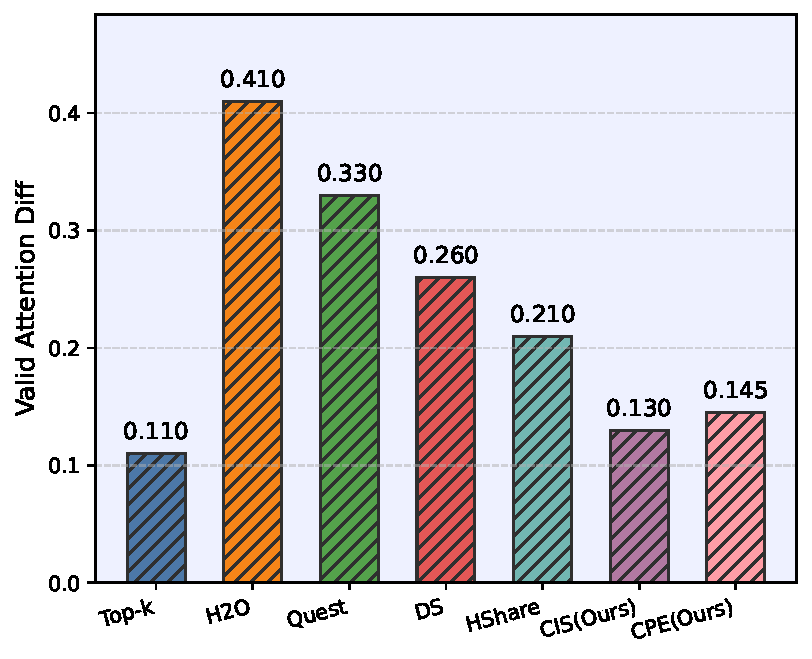
\includegraphics[width=0.305\textwidth]{assets/teaser/attn_diff.pdf}
  }\hfill
  \subfloat[Introduced absolute differences between original attention outputs.]{
  \footnotesize
  \label{fig:teaser_latent_diff}
    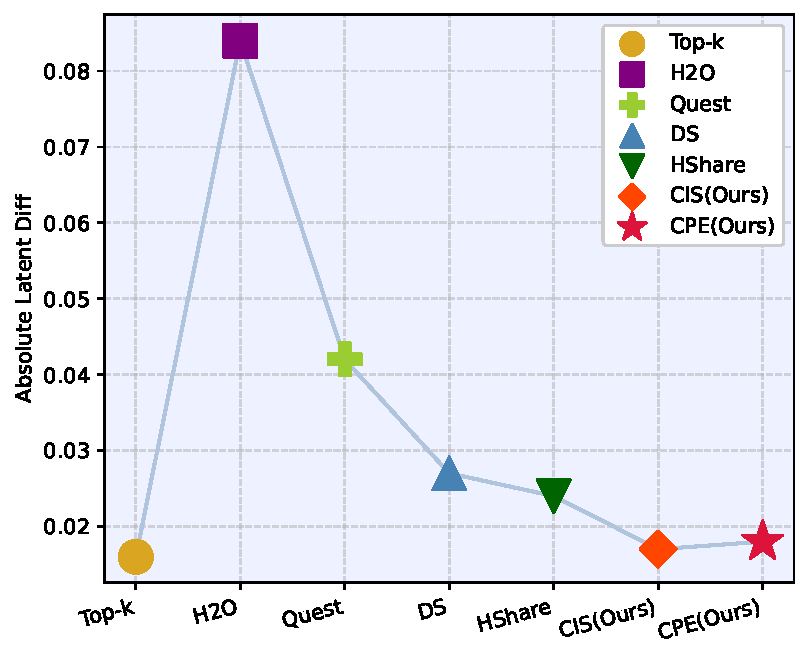
\includegraphics[width=0.305\textwidth]{assets/teaser/latent_diff.pdf}
  }\hfill
  \subfloat[Overall comparisons on accuracy-consumption trade-offs among state-of-the-art baselines.]{
  \footnotesize
  \label{fig:teaser_overall_comp}
    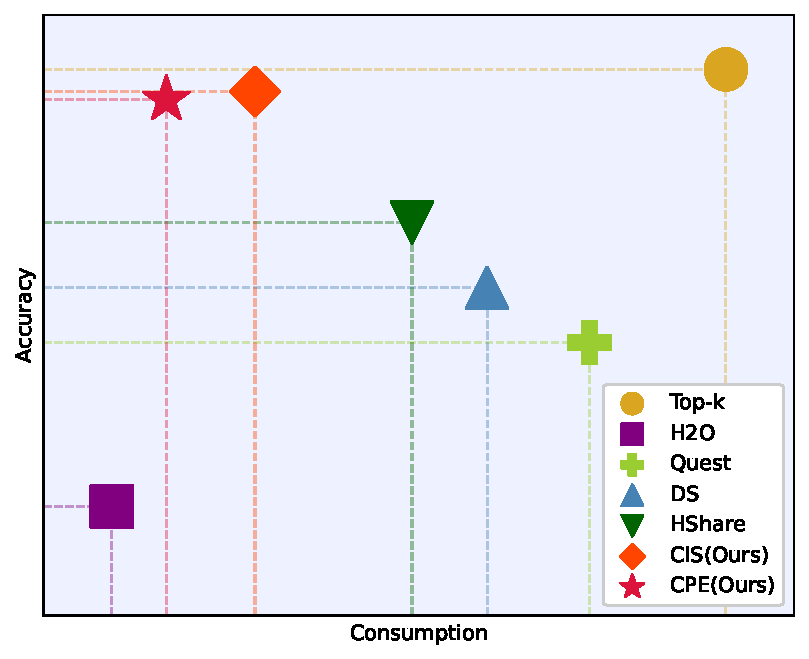
\includegraphics[width=0.305\textwidth]
    {assets/teaser/overall_comp.pdf}
  }
  \vspace{-0.05in}
  \caption{\textbf{Overall analysis of performance and efficiency}. Across induced attention-approximation error and accuracy-efficiency trade-offs, our method consistently surpasses prior SOTA approaches and closely tracks the top-$k$ oracle for optimal KV compression accuracy.}
  \label{fig:teaser}
  \vspace{-0.1in}
\end{figure*}





\iffalse
\begin{figure*}[!t]
    \centering
    \subfigure[Overall comparisons on accuracy and resource consumption among existing techniques.]{
        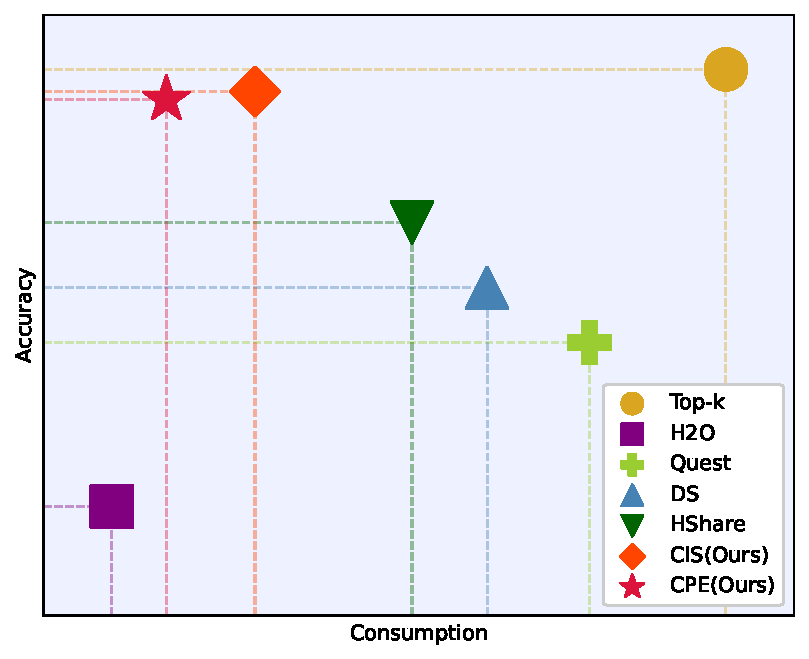
\includegraphics[width=0.305\textwidth]{assets/teaser/overall_comp.pdf}
        %\label{fig:teaser_overall_comp}
    }
    \hfill
    \subfigure[Introduced attention disturbances after filtering attention lgits $<0$.]{
        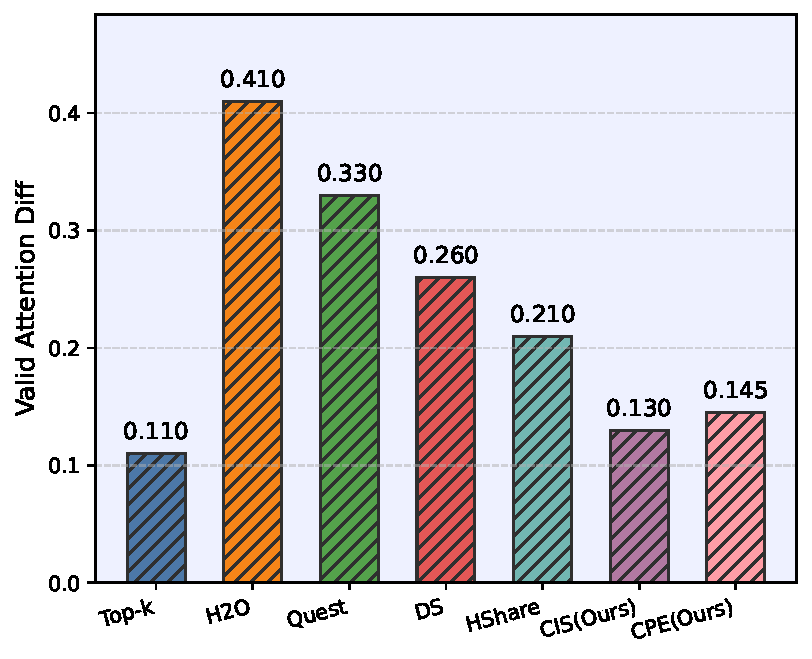
\includegraphics[width=0.305\textwidth]{assets/teaser/attn_diff.pdf}
        %\label{fig:teaser_ppl_elim}
    }
    \hfill
    \subfigure[Introduced absolute differences between original attention outputs.]{
        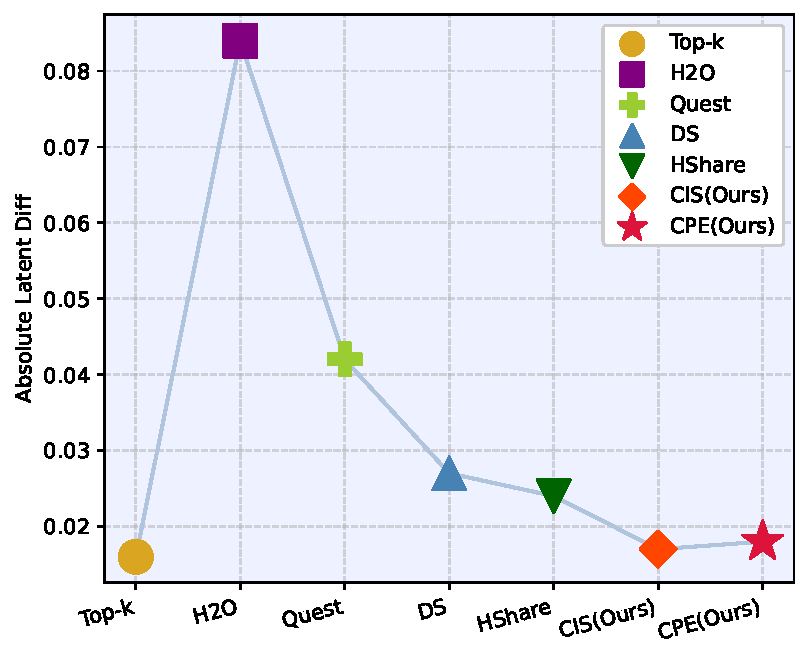
\includegraphics[width=0.305\textwidth]{assets/teaser/latent_diff.pdf}
        % \label{fig:teaser_acc_elim}
    }
    \vspace{-0.1in}
    \caption{Analysis of attention sparsity and its impact. (a) Attention is highly sparse across layers. (b) Perplexity maintains stable when large amounts of low-magnitude attention are eliminated. (c) Accuracy remains robust to large-scale attention pruning.}
    \label{fig:teaser}
    \vspace{-0.1in}
\end{figure*}
\fi




\iffalse
%------------------------------------------------------
\begin{figure*}[!t]
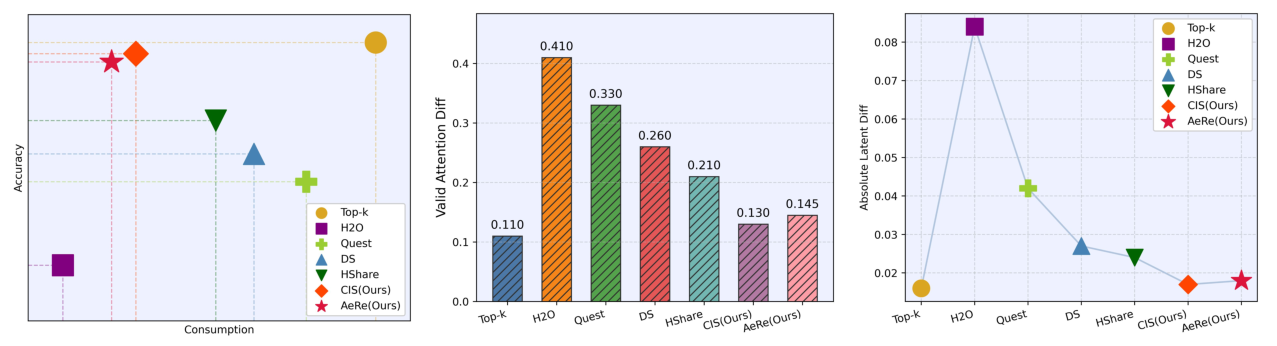
\includegraphics[width=1\textwidth]{assets/Teaser.pdf}
\centering
%\vspace{-1em}
    \caption{\textbf{Distribution of critical indices across heads and layers in LLaMA2-Chat-7B.} We highlight the critical indices in \textcolor{red}{red} and select the critical clusters (\textcolor{green!60!black}{green circles}, without local key tokens) within a range of consecutive queries (\textcolor{violet}{purple box}). Although not strictly contiguous, the critical key indices consistently form stable and dense clusters across multiple heads and layers.}
    \label{fig:teaser}
    %\vspace{-1.5em}
\end{figure*}
%------------------------------------------------------
\fi

Therefore, in this paper, we analyze selection through a \emph{marginal-to–mutual-information} lens and devise a new framework, \textbf{Pre-hoc Sparsity} (PrHS).
Let $\delta$ denote the dropped attention mass (mass of discarded KV entries),
and let $\Delta H$ quantify the induced perturbation of the attention distribution.
We prove that the selection-induced \emph{mutual-information loss} admits an
upper bound that depends only on $\delta$ (Eq.~\eqref{eq:prhs_bound}).
This provides an a-priori error certificate: by constraining $\delta$
before scoring, PrHS instantiates selectors that avoid posterior bias and delivers explicit selection–error control by enforcing conditions that tighten the bound. Consequently, PrHS markedly reduces attention- and output-level perturbations and approaches the oracle frontier in the accuracy–efficiency trade-off (Fig.~\ref{fig:teaser_overall_comp}).
We further quantify deviation from the oracle by $\beta_{\mathrm{th}}$, the
marginal-entropy gap between PrHS and top-$k$; as $\beta_{\mathrm{th}}\!\to\!0$,
PrHS converges to the oracle (Eq.~\ref{eq:limit_to_oracle}; proof in
Sec.~\ref{sec:app_mib_tsa}).



We instantiate three PrHS techniques, Clustered Index Sharing (CIS), Progressive Sliding Attention Window (PSAW), and Early Token Freezing (ETF), each translating a distinct sparsity prior into a PrHS selector. These selectors are then parameterized to tighten the MI upper bound on marginal-entropy error (Eq.~\eqref{eq:prhs_bound}). CIS explores temporal-locality~\cite{wuhshare}: consecutive queries are highly similar. It shares the retrieved set from the top-$k$ oracle across temporally adjacent queries whose embeddings exceed a cosine-similarity threshold, and dilates it by adding neighbors around highest-score indices. PSAW leverages the recency prior~\cite{xiao2023streamingllm,zhang2023h2o}—attention mass concentrates on a local window—and applies a depth-adaptive sliding window that shrinks monotonically with depth, incrementally pruning the candidate KV entries. ETF exploits cross-layer redundancy~\cite{liu2405minicache}: adjacent layers exhibit high KV similarity. ETF freezes stable early tokens to reduce updates. The three selectors act along different axes—time (CIS), depth (PSAW), and layer (ETF)—and compose naturally: CIS seeds the candidate pool with a small budget, then PSAW and ETF intersect their selections with the CIS seed using larger budgets to further prune. Finally, we implement custom CUDA kernels that parallelize index manipulation and sparse-attention computation to minimize runtime overhead. We refer to the combined system as \textbf{CPE}. 

%  relative to state-of-the-art baselines

% within a fixed index radius 

Collectively, CPE delivers competitive reductions in memory footprint and end-to-end latency with substantially improved relative to state-of-the-art (SOTA) baselines (Fig.~\ref{fig:teaser_overall_comp}). Empirically, on LLaMA~\cite{touvron2023llama} and Mistral model families~\cite{jiang2023mistral7b} across GSM8K and CoQA, CIS matches the accuracy of recent SOTA method HShare~\cite{wuhshare} while using only \emph{one-third} of its retrieval complexity. Overall, CPE maintains comparable model quality even with reducing $> \!90\%$ KV-retrieval overhead, while lowering $\sim \! 15\%$ attention FLOPs than prior sparse baselines. On NVIDIA A800-80GB GPUs, CPE attains a $\mathbf{9.9\!\times}$ speedup in attention-operator latency and a $\mathbf{2.8\!\times}$ throughput improvement over original models. Ablation studies in Sec.~\ref{sec:hyper-tune} further confirm that each component contributes reliably. Our contributions are summarized as follows:
\begin{enumerate}[label=\arabic*)]
    \item Rigorous analyses of the mutual information bound from the marginal entropy in KV compression and introduction of Pre-hoc Sparsity towards the accuracy of top-$k$ oracle.
    \item Introduction of CIS, which sustains stable performance at high sharing ratios, together with PSAW and ETF for lossless sparsification of attention computation, all implemented with customized CUDA kernels for parallelization.
    \item Extensive experiments and ablations demonstrating consistent improvements in accuracy, efficiency, and throughput over state-of-the-art baselines.
\end{enumerate}


% We instantiate three PrHS techniques, each with distilled properties from a distinct prior and parameterized to reduce the MI upper bound on marginal-entropy error (Eq.~\eqref{eq:prhs_bound}). Clustered Index Sharing (CIS) explores temporal locality—consecutive queries are highly similar~\cite{wuhshare}—from which we obtain that their most critical entries (positions) cluster (Fig.~\ref{fig:idx_cluster}) and undergo small centroid shifts. CIS shares the critical-index set across temporally adjacent, semantically similar queries (measured by cosine similarity of query embeddings). To preserve recall under shifts, we dilate each shared set by including neighbors within a fixed index radius around highest-score indices, ensuring coverage while enabling aggressive sharing. Progressive Sliding Attention Window (PSAW) leverages the recency prior~\cite{xiao2023streamingllm,zhang2023h2o}: attention mass concentrates on a local window; and the useful tokens shrink with layer depth. PSAW applies a depth-adaptive sliding window that shrinks monotonically with depth, incrementally pruning the candidate set. Building on PSAW, Early Token Freezing (ETF) exploits cross-layer redundancy prior: adjacent layers exhibit high KV similarity~\cite{liu2405minicache}. ETF freezes updates to early tokens once stability criteria are met, further reducing computation and complementing PSAW's incremental pruning. All three techniques are orthogonal and, with appropriately chosen budgets, satisfy the pre-hoc MI bound on approximation error. At inference time, we first apply CIS with a small budget, then apply PSAW and ETF with larger budgets and intersect their selections with CIS to further prune. We implement custom CUDA kernels that parallelize index manipulation and sparse-attention computation to minimize runtime overhead. We refer to the combined system as \textbf{CPE}.


% To championing top-k oracle, we devise a new method, which comprises three complementary techniques. First, noting that critical tokens cluster (\emph{sink effect}, Fig.~\ref{fig:idx_cluster}) and that adjacent queries exhibit \emph{mean-shift} in their critical sets, we propose \textbf{Clustered Index Sharing} (CIS). CIS shares critical indices among semantically similar (measured by cosine similarity in the feature space), temporally adjacent queries. To preserve recall, each shared set is expanded by a fixed index radius to cover local neighbors, yielding near-complete cluster coverage to avoid omission of critical indices, sustaining accuracy under aggressive sharing. Nest, exploiting \emph{progressive information propagation} of LLMs, we introduce \textbf{Progressive Sliding Attention Window} (PSAW) and \textbf{Early Token Freezing} (ETF) to incrementally prune redundant attention with increasing layer depth. Finally, we pair these algorithms with customized CUDA kernels that parallelize index manipulation and sparse-attention computation, minimizing runtime overhead. We refer to the combined system as \textbf{CPE}.



% \section{Related Work}

\paragraph{Reasoning Models}
While traditional LLMs perform well on general tasks, achieving breakthroughs in complex logical reasoning has remained a significant challenge. This bottleneck has recently been addressed by a new class of models named reasoning models designed for long CoT generation.
Pioneered by OpenAI-o1 \citep{openaio1}, DeepSeek-R1 \citep{deepseekr1} leverages Reinforcement Learning with Verifiable Rewards (RLVR) to unlock the model's latent abilities for long CoT generation and high-level reasoning.
These breakthroughs catalyze a subsequent wave of increasingly powerful reasoning models from numerous research labs, including Qwen3 \citep{qwen3}, Gemini-2.5 \citep{gemini2.5}, and GPT-5 \citep{gpt5}. Researchers have employed advanced training strategies to develop increasingly powerful models that mark new milestones.
However, the long-CoT reasoning paradigm introduces significant deployment challenges. Generating lengthy sequences inflates the KV cache, leading to severe memory and computational bottlenecks. This problem is further exacerbated by the models' tendency to overthink \citep{overthinking}. While numerous approaches have been proposed to develop more efficient reasoning models \citep{overthinking1, speculativecot, jiang2025think}, they often focus on shortening the CoT, which risks constraining the model's reasoning capability. Developing more effective methods remains an open challenge.



\paragraph{KV Cache Compression}
KV cache compression is a widely used technique for improving the efficiency of LLM inference by retaining essential contextual information under limited memory budgets. Existing methods typically exploit attention patterns to identify and evict less important tokens, or adopt more explicit objectives that approximate attention output similarity \citep{ada}.
Despite their effectiveness in long-input scenarios, these eviction-based methods suffer from irreversible information loss and often incur non-trivial computational overhead, making them less suitable for long-output generation. To address this, more recent approaches construct compact representations instead of directly discarding tokens, for example through semantic chunking \citep{chunkkv} or cross-layer merging \citep{minicache}. Other methods periodically refresh cached representations to mitigate permanent information loss \citep{refreshkv}. While promising, these techniques typically introduce additional computation or architectural complexity. In contrast, our work focuses on a fundamentally lightweight KV cache compression method specifically tailored to the long-output setting of reasoning models.


%\vspace{-0.05in}
\section{Problem Formulation}

This section introduces several variables and notation used throughout our analysis. For convenience, Table~\ref{tab:notation} summarizes the key symbols and their meanings.

\subsection{LLM Inference}
\label{sec:inference_background}
% \vspace{-0.05in}

To demonstrate the inference bottlenecks that KV compression aims to address, we present the inference process, consisting of two stages—prefill and decode—using the standard transformer architecture with multi-head attention~\cite{vaswani2017attention}.



\paragraph{Multi-head Attention} Let the input token embeddings for head $h$ be $\bx^h=[\bx_1^h;\dots;\bx_L^h]\in\mathbb{R}^{L\times d}$. With $H$ heads and per-head dimension $d$, for each token $i$ and head $h\in{1,\dots,H}$,
\begin{equation}
\label{eq:qkv-proj}
    \bq_i^h \!=\! \bx_{i} \bW_Q^h, \, \mathbf{k}_i^h \!=\! \bx_{i} \bW_K^h, \, \bv_i^h \!=\! \bx_{i} \bW_V^h, \,
\end{equation}
where $\bq_i^{h}, \bk_i^h, \bv_i^h \in \mathbb{R}^{d}$ and $\bK^h=[(\bk_1^h)^\top;\dots;(\bk_L^h)^\top], \bV^h=[(\bv_1^h)^\top;\dots;(\bv_L^h)^\top]\in\mathbb{R}^{L\times d}$ to form the KV cache. Attention weights for token $t$ in head $h$ over indices $i\in{1,\dots,t}$ and the attention output for step $t$ are
\begin{equation}
\label{eq:attn_eq}
    A_i^h(\bq_t^h) \!=\! \frac{\exp\! \big((\bq_t^{h})^\top \bk_i^h/\sqrt d\big)}{\sum_{j=1}^{t}\exp\!\big((\bq_t^{h})^\top \bk_j^h/\sqrt d\big)}, \; 
    \mathbf{y}_t^h \!=\! \sum_{i=1}^{t} A_i^h(\bq_t^h)\,\bv_i^h .
\end{equation}
Since all heads operate the same, we omit the head index for brevity in the following context, unless explicitly mentioned.


\paragraph{Prefill} The prompt is processed once to construct and cache $(\bK,\bV)$, which is reused during subsequent decoding~\cite{ott2019fairseq}.

\paragraph{Decode} Only the new token is processed while reusing the cached $\bK$ and $\bV$ from previous steps for each head.

\paragraph{Bottlenecks} From Eq.~\eqref{eq:attn_eq}, the per-step attention FLOPs (score computation and value aggregation) scale as $\mathcal{O}(Htd)$, and the KV cache also scales as $\mathcal{O}(Htd)$. This linear growth in $t$ constitutes the primary compute and memory bottleneck for long-context inference.

\begin{table}[t]
\caption{Summary of key variables and notation.}
\label{tab:notation}
\centering
\renewcommand{\arraystretch}{1.15}
\begin{tabularx}{\columnwidth}{lX|lX}
\toprule
$\bx$ & Input token embedding 
& $\bq,\,\bk,\,\bv$ & Query, key, value \\
$L$ & Input length
& $d$ & Per-head dimension \\
$H$ & Number of heads
& $A(\cdot)$ & Attention weight \\
$\bK, \bV$ & KV cache matrices
& $t$ & Step count\\
$\mathcal S$ & Selector returning a subset of indices
& $S_t$ & Selected KV index set at step $t$ \\
$N$ & KV budget (sparsity: $N/t$)
& $\tau(\cdot)$ & Retained attention mass \\
$\delta(\cdot)$ & Dropped attention mass
& $I_{\mathrm{full}}, I_{\mathcal S}$ & MI under full attention vs.\ TSA \\
$g(\cdot)$ & MI-loss bound function
& $\delta^*(\cdot)$ & Oracle (top-$k$) dropped mass \\
\bottomrule
\end{tabularx}
\end{table}


\subsection{Token-sparse Attention and Key-value Sharing}
\label{sec:prob_def}

KV compression mitigates the aforementioned bottlenecks by exploiting attention sparsity—a small subset of critical KV entries is selected to approximate full attention. This improves efficiency at the cost of approximation error. To evaluate accuracy–efficiency trade-offs across KV compression methods, and following prior work~\cite{xiao2024duoattention,wu2024tokenselect,wuhshare,liu2025freekv}, we formalize decoding with a limited KV set under a unified \emph{token-sparse attention} (TSA) concept, and then define \emph{KV sharing} as a special case that streamlines TSA selection.


\textbf{Definition 3.1} (Token-sparse attention, informal).
\textit{At decoding step $t$, with KV budget $N < t$, a selector $\mathcal{S}$ outputs an index set $S_t \subseteq [t] \coloneqq \{1,\dots,t\}$ with $|S_t| = N$. The corresponding key/value matrices are restricted to these indices, $\bK_{S_t}$ and $\bV_{S_t}$. Attention is computed only between $\bq_t$ and $\bK_{S_t}$ (cf. Eq.~\eqref{eq:attn_eq}), and the output uses $\bV_{S_t}$. The sparsity ratio at step $t$ is $N/t$.}


\textbf{Definition 3.2} (Key-value sharing). \textit{Given indices $S_i$ retrieved by $\mathcal S$ at an anchor step $i$ in TSA, a later token at step $j$ may directly reuse them, denoted $S_j \leftarrow S_i$. In this case, $S_j$ is utilized to construct $\bK_{S_j}$ and $\bV_{S_j}$.}

\textbf{Discussion}. Different TSA instantiations correspond to different selectors $\mathcal{S}$, and exhibit distinct accuracy–efficiency trade-offs under a fixed budget. For example, imprecise selection that admits many low-contribution pairs can crowd out salient entries, increasing approximation error and degrading model performance. This failure mode is analogous to erroneous KV sharing across steps whose truly critical sets have little overlap. Moreover, selectors rely on different criteria~\cite{liu2024hashevict,zhang2023h2o,sun2024shadowkv} (e.g., similarity heuristics, learned scores, recency rules), and the mechanism used to enforce these criteria determines selection complexity and entry-retrieval efficiency. Consequently, an effective TSA selector must balance accuracy (retained mass) and retrieval overhead (selection complexity).



\vspace{-0.05in}
\subsection{Information Loss Quantification}
\label{sec:info_bound}

To evaluate the accuracy of TSA selectors, we quantify the information loss—information gap between full attention and TSA—via a mutual-information (MI) bound, and pair it with retrieval-efficiency analysis to guide algorithm design. We first derive the MI bound as a function of dropped attention mass, which implies that the top-$k$ oracle attains the best accuracy under a fixed budget. However, it incurs prohibitive selection cost due to explicit attention evaluation. Practical selectors approximate this oracle for efficiency and thus incur additional MI loss. We then formalize selector design as an optimization problem towards minimizing the MI-loss gap relative to the top-$k$ oracle subject to retrieval constraints. Finally, we show that PrHS-based selectors remove posterior bias and, with design-time error control, nearly preserve top-$k$ accuracy without additional retrieval cost, thereby outperforming PoHS selectors.

\paragraph{Mutual-information Bound} In TSA, a selector $\mathcal S$ keeps $N$ KV entries and drops the rest. Our core result (Sec.~\ref{sec:app_uib}) is that the MI loss induced by TSA depends only on the \emph{dropped mass}, independent of selector instantiations. Intuitively, preserving (nearly) the same total attention mass as full attention preserves (nearly) the same information. Hence, MI loss admits a unified characterization in terms of dropped mass. For a query $\bq$, define the retained and dropped attention mass
\begin{equation}
    \tau_{\mathcal S}(\bq)=\sum_{i\in\mathcal S}A_i(\bq), \quad \delta_{\mathcal S}(q)=1-\tau_{\mathcal S}(\bq).
\end{equation}
Let $I$ denote the MI loss measure. For any $\bq$, the MI loss between full attention $I_{\mathrm{full}}$ and selector $\mathcal{S}$ satisfies
\begin{equation}
\label{eq:mi_bound}
\begin{aligned}
    0 \, \le \, & I_{\mathrm{full}}(\bq)-I_{\mathcal S}(\bq) \, \le \, g\big(\delta_{\mathcal S}(\bq)\big), \\
    \text{where} &\quad g(\delta) \coloneqq 2\left[h_{\mathrm b}(\delta)+\delta\log L\right].
\end{aligned}
\end{equation}
Here $h_{\mathrm b}$ is the binary entropy function and $L$ the number of eligible positions (proved in Sec.~\ref{proof:MI_bound}). 

\paragraph{Top-k Oracle and Optimization Goal} The top-$k$ oracle $\mathcal S^{*}(q)\!=\!\operatorname*{Top}_N \!\big(A(\bq)\big)$ minimizes the bound by maximizing retained mass under a fixed budget $N$:
\begin{equation}
% \label{eq:topk_oracle}
\begin{aligned}
\mathcal S^{*}(\bq)
\!\in\! \operatorname*{arg min}_{S\subseteq [t],\, |S|=N}
g\!\left(1\!-\!\!\sum_{i\in S} A_i(\bq)\right)
\!=\!
\operatorname*{arg max}_{S\subseteq [t],\, |S|=N}
\sum_{i\in S} A_i(\bq).
% \;=\;
% \operatorname*{Top}_{N}\!\big(A(\bq)\big).
\end{aligned}
\end{equation}
However, evaluating $A(\bq)$ exactly incurs prohibitive selection cost. Practical selectors (PoHS or PrHS) approximate $A(\bq)$ for efficiency and thus incur additional MI loss. We therefore pose the goal of selector optimization as
\begin{equation}
\label{eq:selector_opt}
\min_{}\; % \theta\in\Theta
\mathbb{E}\!\left[\, I_{\mathcal S^{*}}(\bq)\;-\;I_{\mathcal S}(\bq) \,\right]
\;\; \text{s.t.}\;\; |S^*(\bq)|=|S(\bq)|=N,
\end{equation}
i.e., minimize the MI-loss gap relative to the top-$k$ oracle under constrained budget, where the expectation is over queries $\bq$.


\paragraph{PoHS Selector $\mathcal S_D$}
% \label{sec:pohs_bias}
$\mathcal S_D(\bq)\!=\!\operatorname*{Top}_n(\widehat A_D(\bq))$ replaces $A(\bq)$ with its surrogate $\widehat A_D(\bq)$ derived from posterior side information $D$ (e.g., token ages, sketches), and suffers \emph{posterior bias} measured by the total-variation distance
\begin{equation}
\label{eq:pohs_bias}
    \varepsilon_{D}(\bq)\coloneqq \tfrac12\|A(\bq)-\widehat A_D(\bq)\|_1 .
\end{equation}
The extra dropped-mass gap satisfies $\delta_{\mathcal S_D}(\bq) \le \delta^{*}(\bq)+2\varepsilon_{D}(\bq)$, which, by the monotonicity\footnote{Without loss of generality, in this paper, we restrict the domain of $g$ to the interval (0, L/(1+L)] to ensure its monotonicity, where L denotes the current text length. Note that as $L$ grows large,  $L/(1+L)$ will approach $1$, which renders the previous restriction reasonable.} of $g$ in Eq.~\eqref{eq:mi_bound}, lifts the MI loss bound to
\begin{equation}
\label{eq:posh_bound}
    I_{\mathrm{full}}(\bq)-I_{\text{post}}(\bq)\ \le\ g\big(\delta^{*}(\bq)+2\varepsilon_{D}(\bq)\big).
\end{equation}
Thus, when the surrogate under- or over-scores tokens (large $\varepsilon_D$), the selected set retains less probability mass than the oracle and loses more information. We formalize both TDO and QAA from Sec.~\ref{sec:intro} as PoHS instances. In general, TDO induces larger $\varepsilon_D$ than QAA (worse accuracy) but avoids explicit evaluation of $A(\bq)$ (lower retrieval cost). Proofs are provided in Sec.~\ref{sec:app_tech_lemmas}. 



\paragraph{PrHS Selector $\mathcal S_{pre}$} $\mathcal S_{pre}$ selects critical set \emph{without explicitly computing} $A(\bq)$ and controls a \emph{theoretical error} $\beta_{\mathrm{th}}(q)\!\ge\!0$ that satisfy
\begin{equation}
\label{eq:prhs_bound}
\begin{aligned}
    \tau_{\mathrm{pre}}(\bq)\! \ge\! \tau^{*}(\bq)-&\beta_{\mathrm{th}}(\bq) \Longleftrightarrow \delta_{\mathrm{pre}}(\bq)\! \le\! \delta^{*}(\bq)\!+\!\beta_{\mathrm{th}}(\bq), \\
    \text{with} \quad I_{\mathrm{full}}(\bq)-&I_{\mathrm{pre}}(\bq)\ \le\ g\big(\delta^{*}(\bq)+\beta_{\mathrm{th}}(\bq)\big).
\end{aligned}
\end{equation}
As $\beta_{\mathrm{th}}(q)\!\to\!0$, the bound \emph{converges to the top-$k$ oracle}
\begin{equation}
\label{eq:limit_to_oracle}
I_{\mathrm{full}}(\bq)\!-\!I_{\mathrm{pre}}(\bq)
\!\le\!
g\big(\delta^{*}(\bq)\big)\!\le\!g\big(\delta^{*}(\bq)+2\varepsilon_{D}(\bq)\big),
\end{equation}
explicitly improving on PoHS by eliminating posterior bias. Detailed formulations are in Sec.~\ref{sec:app_mib_tsa}. Moreover, PrHS selectors can partially (CIS) or fully (PSAW, ETF) avoid computing $A(\bq)$ and the associated retrieval, improving accuracy without compromising efficiency.



% Exploiting PrHS thus provides better performance than PoHS when $\beta_{\mathrm{th}}$ is appropriately bounded, which aligns with the promised posterior-bias removal in \emph{design time}. Detailed formulations are shown in Appendix~\ref{sec:app_mib_tsa}. Moreover, PrHS selectors can partially (CIS) or fully (PSAW and ETF) avoid the computation of $A(\bq)$ and its corresponding retrieval  as PoHS selectors, making PrHS selectors improve accuracy without compromising efficiency. 

% Empirically, our CPE achieves higher accuracy than the recent advanced QAA technique, Double Sparsity~\cite{yang2024post}, while only requiring 1/15 of its selection complexity.









\newcommand{\bs}{\mathbf{s}}
%------------------------------------------------------
\begin{figure*}[!t]
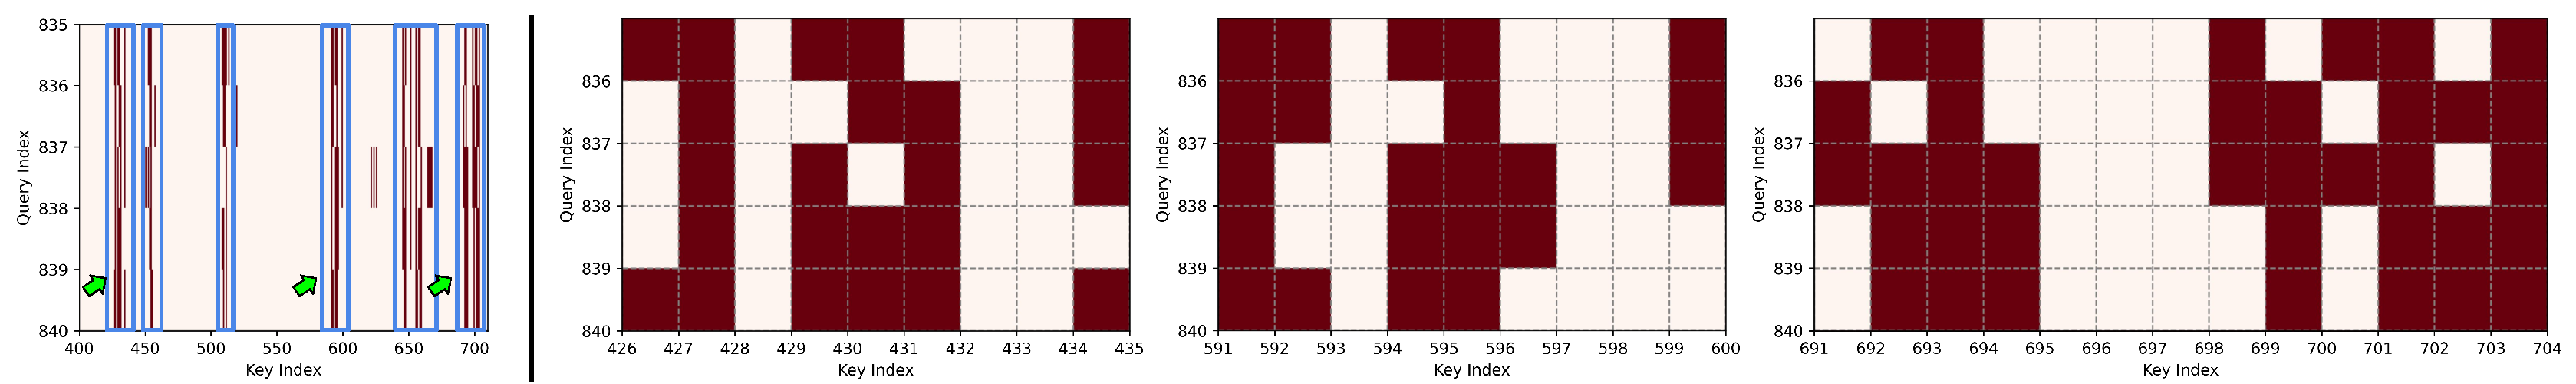
\includegraphics[width=1\textwidth]{assets/attn-cluster.pdf}
\centering
%\vspace{-0.5em}
    \caption{\textbf{Distribution of critical indices in LLaMA2-7B-Chat (Layer 10, Head 2).} For each query, we retrieve 64 critical indices using the top-$k$ oracle on WikiText2. Columns show five temporally adjacent queries with cosine similarity $>\!0.8$. \emph{Left}: overall distribution across keys 400–710; clusters are outlined in \textcolor{blue}{blue boxes}. \emph{Right}: zoom-ins of three clusters (annotated by \textcolor{green}{green arrows} in the left) at keys 426–436, 591–700, and 691–704. Critical indices are in \textcolor{red}{red}.}
    \label{fig:attn-cluster}
    \vspace{-0.5em}
\end{figure*}
%------------------------------------------------------

%  from the same layer–head


%\vspace{-0.05in}
\section{Observations and Properties}
%\vspace{-0.05in}
\label{sec:observations}

While empirical priors (temporal locality, recency, cross-layer redundancy) are suggestive, PrHS requires \emph{query-independent} design rules that can be applied pre-hoc without full attention. Accordingly, from the transformer’s mechanics we derive two properties: (i) clustered locality and among-query continuity of critical indices, and (ii) progressive cross-layer propagation of information. These properties motivate our selector parameterization and, in Sec~\ref{sec:method}, yield a retained-mass guarantee $\tau_{\mathrm{pre}}\!\ge\!\tau^*-\beta_{\mathrm{th}}$, which translates to MI bounds via Eq.~\eqref{eq:mi_bound}.


%------------------------------------------------------
\begin{figure}[!t]
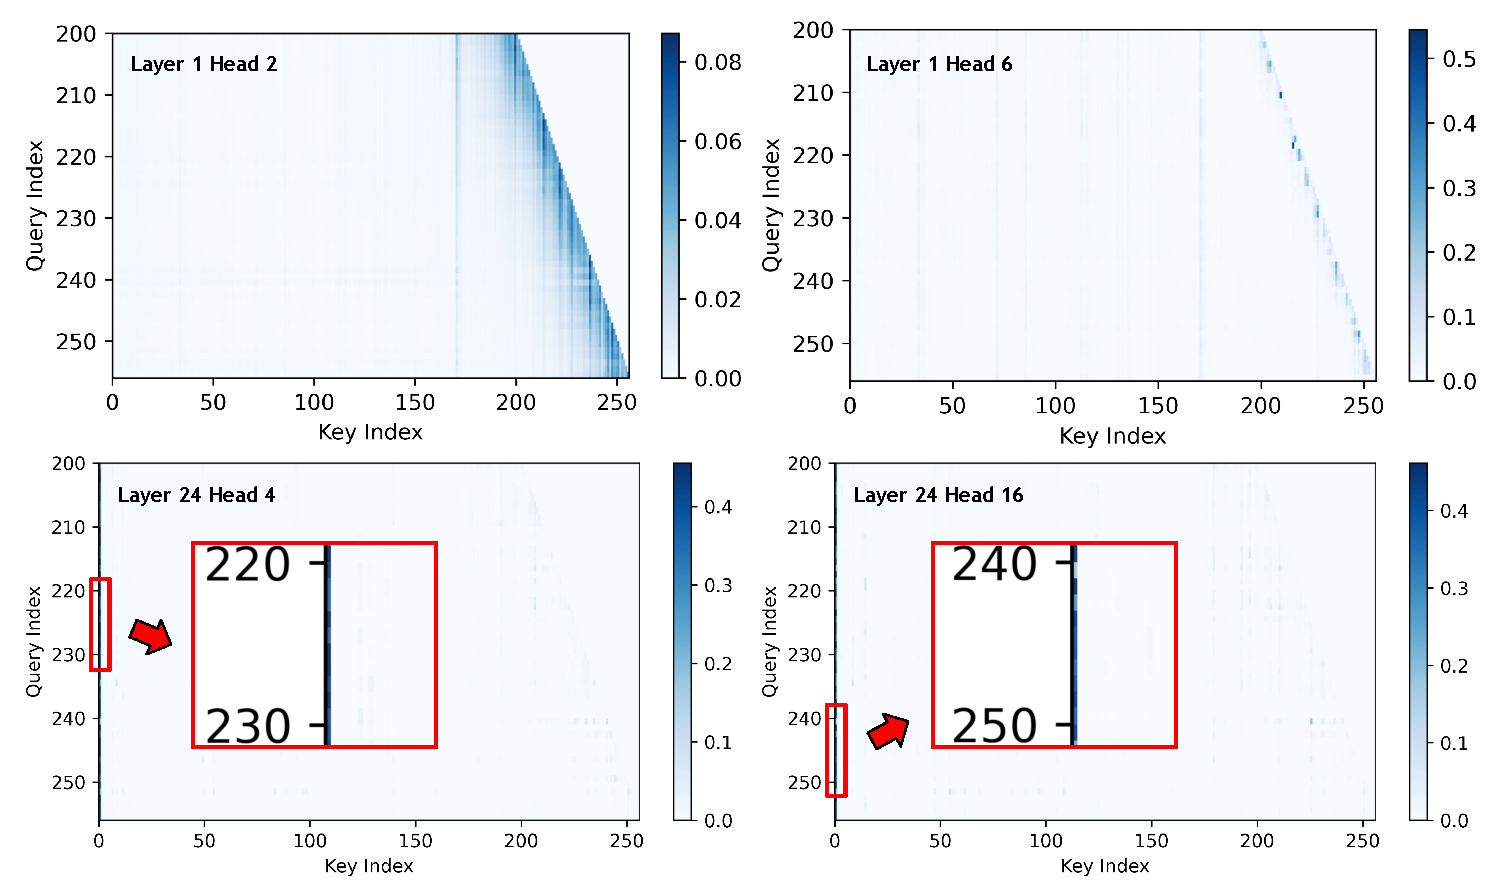
\includegraphics[width=0.45\textwidth]{assets/attn-distribution.pdf}
\centering
\vspace{-0.5em}
    \caption{\textbf{Attention distribution on LLaMA2-7B-Chat.} Heatmaps across representative layer–head pairs, with darker color indicating stronger attention.}
    \label{fig:attn_dis}
    \vspace{-1em}
\end{figure}
%--------

\subsection{Observation 1: Critical Tokens Exist in Clustered Manners}

Prior work~\cite{sun2024shadowkv,li2024snapkv,wuhshare} shows that consecutive decoding queries are close in embedding space and often share critical indices, which motivates KV sharing strategies. However, \emph{per-head} selections can still vary markedly, and the overlap between selected indices remains small even for high cosine similarity between queries~\cite{wu2024tokenselect}, leading to
suboptimal sharing. For example, HShare~\cite{wuhshare} shares indices directly, missing many truly critical indices at high sharing ratios.
To bridge this gap, we observe that critical indices organize into a small number of clusters that persist across adjacent queries, providing a more stable sharing
unit than individual indices. 

\begin{property}[Among-query Property]
\label{prop:among-query}
For two semantically similar consecutive queries, the centroids of their critical-token clusters undergo a smooth mean shift along the sequence axis.
\end{property}

As shown in Fig.~\ref{fig:attn-cluster}, when the cosine similarity between $q_t$ and $q_{t+1}$ exceeds $0.8$, critical indices concentrate into a few clusters; although cluster centers and spreads shift slightly, the cluster-level overlap remains large. Our theoretical analysis further shows that these clusters satisfy a mean-shift (bounded drift) property, formalized in \textbf{Theorem}~\ref{the:mean-shift}.

\begin{theorem}[Centroid Drift]
\label{the:mean-shift}
Consider the scaled dot-product self-attention (cf. Eq.~\eqref{eq:attn_eq}) with fixed keys $\{\bk_j\}_{j=1}^t$, attention weights $A_j(\bq_t)$ for key $\bk_j$, and let $\{p_j\}_{j=1}^t$ be scalar token positions with
$\mathrm{diam}\,\mathcal{P}:=\max_j p_j-\min_j p_j$ for $\mathcal{P}=\{p_j\}$. Define the sequence-axis centroid $c(\bq_t)=\sum_{j} A_j(\bq_t)\,p_j$. For $\bq' = \bq_t + \Delta$ with $\|\Delta\|\ll 1$,
\begin{equation}
\label{eq:centroid_shift}
    c(\bq') = c(\bq_t) + O(\|\Delta\|),
\end{equation}
\textit{i.e., the attention centroid moves in a Lipschitz-continuous fashion with respect to the query. In particular, $|c(\bq')-c(\bq_t)| \le (\mathrm{diam}\,\mathcal{P})\,\frac{\max_j \|\bk_j\|}{\sqrt d}\,\|\Delta\|$.}
\end{theorem}
The drift is $\mathcal{O}(\|\Delta\|)$ with Lipschitz modulus
$L \le (\mathrm{diam}\,\mathcal{P})\,\max_j \|\mathbf{k}_j\|/\sqrt{d}$.
This smooth drift is consistent with empirical attention patterns and with
StreamingLLM’s “keep a few initial tokens” observation~\cite{xiao2023streamingllm}.


In summary, \textbf{across heads and layers, the critical tokens of successive similar queries form dense, localized clusters}. We call this the \textbf{sink effect}: \textit{tokens near a high-attention location inherit elevated attention due to semantic proximity}. Exploring the effect enables explicit control under PrHS, our CIS operationalizes this by dilating shared sets to cover the local cluster and compensate for centroid drift, avoiding full per-head re-retrieval. Detailed proofs are in \textbf{Appendix A}.



\subsection{Observation 2: Information Propagates Progressively Among Layers}

Locality-bias analyses~\cite{zhang2023h2o,ge2023fastgen} show that attention is
sharply concentrated locally within a narrow window around the current query
and the sink token, across diverse prompts (Fig.~\ref{fig:attn_dis}).
This suggests that the current token draws most information from recent tokens,
whereas the sink token acts as an attractor rather than conveying semantic content.
Viewed in isolation, such constrained receptive fields would only support short-term memory for LLMs, seemingly at odds with their strong long-context performance.
Moreover, recent studies~\cite{cai2024pyramidkv,wan2024d2o,gao2023empower} show that:
across layers, intermediate tokens incrementally absorb the semantics of their relevant predecessors; by higher layers, a mid-sequence token encodes both its own content and a compressed synopsis of earlier, distant tokens.
It means that stacking transformer layers realizes long-range dependency paths through chains of neighboring tokens even when no individual layer attends broadly.
Consequently, salient long-distance information is distilled into nearby carrier
tokens, reducing the marginal importance of many earlier ones; hence,
later layers need not re-scan the full prefix.
Building on this insight, PSAW and ETF prune KV entries whose instantaneous (per-layer) and accumulated (cross-layer) attention mass fall below preset thresholds, ensuring that the total dropped mass remains within $\beta_{\mathrm{th}}$; by Eq.~\eqref{eq:mi_bound}, this certifies a bounded MI loss.
We formalize these guarantees in \textbf{Appendix C-D}.


% Prior work~\cite{sun2024shadowkv,li2024snapkv,wuhshare} shows that adjacent queries are close in embedding space and share many critical indices, motivating KV sharing techniques. However, \emph{per-head} selection among these queries can still differ markedly, and overlap remains small even when queries are nearly identical~\cite{wu2024tokenselect}, yielding suboptimal KV sharing results. For example, HShare~\cite{wuhshare} shares indices directly, missing many truly critical indices at high sharing ratios. To close this gap, we observe that critical indices form \emph{clusters} that persist across adjacent queries, and formalize this in Property~\ref{prop:among-query}.

%Locality-bias analyses \cite{zhang2023h2o,ge2023fastgen} show that, attention is sharply local-concentrated within a narrow window around the query plus the sink token, regardless of prompts, as shown in Fig.~\ref{fig:attn_dis}. This indicates that the current token absorbs most of information from recent tokens, as sink token is a placeholder and does not convey any actual content. Viewed in isolation, such constrained receptive fields would only support short-term memory for LLMs, seemingly at odds with their strong long-context performance. While recent studies~\cite{cai2024pyramidkv,wan2024d2o,gao2023empower} show that: across layers, intermediate tokens incrementally absorb the semantics of its relevant predecessors; by higher layers, a mid-sequence token encodes both its own content and a compressed synopsis of earlier, distant tokens. Thus, stacking transformer layers realizes long-range dependency paths through chains of neighboring tokens, even when no individual layer attends broadly. As such, salient long-distance information is distilled into nearby carrier tokens, reducing the marginal importance of many earlier ones. Therefore, \textit{later layers need not re-scan the full prefix}. PSAW and ETF prune KV entries whose instantaneous (per-layer) and accumulated (cross-layer) attention mass fall below preset thresholds, so that the total dropped mass stays within $\beta_{\mathrm{th}}$, following the bounded MI loss in Eq.~\eqref{eq:mi_bound}. We formalize these guarantees (Theorem~\ref{the:error_bound}) once PSAW and ETF are in place.


%------------------------------------------------------
\begin{figure}[!t]
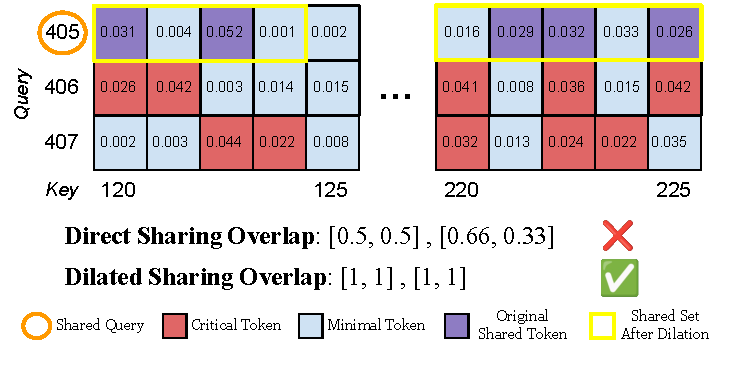
\includegraphics[width=0.48\textwidth]{assets/index-frag.pdf}
\centering
\vspace{-0.5em}
    \caption{\textbf{Critical-index set (CIS) dilation.} For three adjacent queries (405–407), we examine two key-index clusters $[120,125]$ and $[220,225]$. Critical tokens from query 405 are shared to queries 406 and 407. Overlap is measured as $\frac{\text{Number of True Positive}}{\text{Number of Critical Tokens}}$. Tokens in \textcolor[HTML]{A64DFF}{violet} are also critical for query 405.}
    \label{fig:index-frag}
    \vspace{-1em}
\end{figure}
%--------

\vspace{-0.05in}
\section{Proposed Method and Implementation}
\vspace{-0.05in}
\label{sec:method}

In this section we present CPE. First, \textbf{CIS} (from Observation~1) enables efficient head-level KV sharing across adjacent queries. Next, \textbf{PSAW} and \textbf{ETF} (from Observation~2) prune redundant attention by shrinking visible attention window and freezing early token updates, respectively, with theoretical error guarantees. We also describe CUDA kernels for parallel index manipulation and sparse attention.



\subsection{Clustered Indices Sharing (CIS)}
\label{sec:cis}

CIS performs head-level KV sharing with dilated shared set among semantically similar, and temporally adjacent queries. By \textbf{Observation}~1 and \textbf{Theorem}~\ref{the:mean-shift}, the critical clusters for such queries undergo only small mean shifts relative to a reference query. Therefore, exhaustive per-query head-level retrieval is unnecessary. We first partition the sequence into fixed-length blocks and restrict sharing to within a block to enforce temporal adjacency, where semantically similar but non-adjacent (cross-block) queries are not shared. 


\paragraph{Selection Criteria}
Within each block, the first query serves as an initial reference and computes its critical indices across layers and heads. Following~\cite{zhang2023h2o,wuhshare} and the locality bias in \textbf{Observation~2}, selection budgets are allocated to three token groups: initial (sink) tokens, local tokens, and salient middle tokens. Let $C_{\text{sink}}$ and $C_{\text{local}}$ denote the numbers of sink and local tokens, respectively. At decoding step $t$, we obtain the middle set with a budget $k$ by applying the top-$k$ oracle over positions $[C_{\text{sink}}, t\!-\!C_{\text{local}}]$, excluding the sink and local regions. This yields $S_t^*=\{p_{t,i}\}_{i=1}^{k}$, where $p_{t,i}$ is sorted and selected in descending order of attention weight. The per-head critical index set is $\mathcal{C}_t=\{1,\ldots,C_{\text{sink}}\} \cup S_t^* \cup \{t-C_{\text{local}}+1,\ldots,t\}$, with a total size $C=C_{\text{sink}}+k+C_{\text{local}}$.




\paragraph{Similarity Criteria}
For a later query, if there exists an earlier query $j$ whose cosine similarity exceeds a threshold $\tau$, KV sharing is performed. We measure similarity as
\begin{equation}
\begin{aligned}
\label{eq:cos_sim}
\mathsf{sim}(i,j)=\frac{\bq_{i}^{\!\top} \; \bq_{j}}{\|\bq_{i}\|\,\|\bq_{j}\|}.
\end{aligned}
\end{equation}
If multiple candidates satisfy $\mathsf{sim}(i,j)>\tau$, we choose the most recent such $j$ to preserve adjacency. Varying $\tau$ trades throughput for accuracy.

\paragraph{Neighboring Dilation}
Naive sharing ignores centroid drift (Eq.~\eqref{eq:centroid_shift}) and yields fragmented critical sets (Figs.~\ref{fig:attn-cluster}, \ref{fig:index-frag}), missing true positives for shared queries. We therefore dilate the $m$ highest-weight indices in $S_t^*$ (with $m\!\le\!k$) by their $\pm r$ neighbors:
\begin{equation}
\label{eq:neighboring}
\begin{aligned}
\hat S_t 
\;=\; 
S_t^* 
\;\cup\;
\bigcup_{i=1}^{m}\big\{p_{t,i}+j \;|\;-r\le j\le r\,\big\}.
\end{aligned}
\end{equation}
As shown in Fig.~\ref{fig:index-frag}, dilation substantially increases true-positive overlap and achieves complete coverage compared to direct sharing. Moreover, restricting dilation to the top-$m$ indices mitigates attention pollution from adding excessive low-weight tokens, as detailed in Sec.~\ref{sec:cis-dilation}.

\paragraph{Analysis}
\label{sec:cis_analysis}
Theoretically, CIS also turns Property~\ref{prop:among-query} into a pre–hoc guarantee as proved in Theorem~\ref{thm:cis-main} (detailed in \textbf{Appendix A, A3}). 

\begin{theorem}[CIS Retained–Mass and MI Guarantee]
\label{thm:cis-main}
For a reference query $q$ and its shared set $\hat S_t$ dilated with $\pm r$ neighbors 
around the top-$m$ winners ($m<k$), as in~\eqref{eq:neighboring}. Let $s(\tau)$ be any radius that covers the centroid drift implied by \eqref{eq:centroid_shift}, for any later query $\bq'$ with $\mathsf{sim}(\bq,\bq')\ge \tau$ (cosine similarity), if $r\!\ge\!s(\tau)$, then:
\begin{equation}
\begin{aligned}
\tau_{\mathrm{pre}}(\bq') \;\ge\; \tau^*(\bq') - \beta_{\mathrm{th}}(\tau),
\quad 
\beta_{\mathrm{th}}(\tau) \;\le\; 2\,\Delta_{\mathrm{att}}(\tau), \\
\text{where} \quad \Delta_{\mathrm{att}}(\tau)\!:=\!\big\|A(\bq')\!-\!A(\bq)\big\|_1 
\!\le\! \frac{2\,K_{\max}}{\sqrt d}\sqrt{2\!-\!2\tau}.
\end{aligned}
\end{equation}
Consequently, the MI gap obeys the pre–hoc bound as in~\eqref{eq:prhs_bound}, where $\beta_{\mathrm{th}}^{\mathrm{CIS}}(\tau)=2\Delta_{\mathrm{att}}(\tau)$. \emph{If }$r<s(\tau)$\emph{, the same holds with }\(2\Delta_{\mathrm{att}}\) \emph{replaced by } 
\(2\Delta_{\mathrm{att}}(\tau)+\varepsilon_{\mathrm{drift}}(\bq,\bq';m,r)\), 
where \(\varepsilon_{\mathrm{drift}}\) is the residual mass outside the chosen radius.
\end{theorem}



In short, by tying $(\tau,m,r)$ to Lipschitz continuity and the observed mean-shift of clustered indices, CIS achieves a controlled $\beta_{\mathrm{th}}^{\mathrm{CIS}}$ and therefore a tightened MI gap. Empirically, the mean-shift rate saturates once the prefix length exceeds a moderate scale; i.e., within a reasonably large block, cluster distributions of aligned queries become nearly identical. During experiments, $s\geq 8$ and $\mathsf{sim} \geq 80\%$ can still satisfy competitive performance, which corresponds to aggressive sharing ratios.


%------------------------------------------------------
\begin{figure*}[!t]
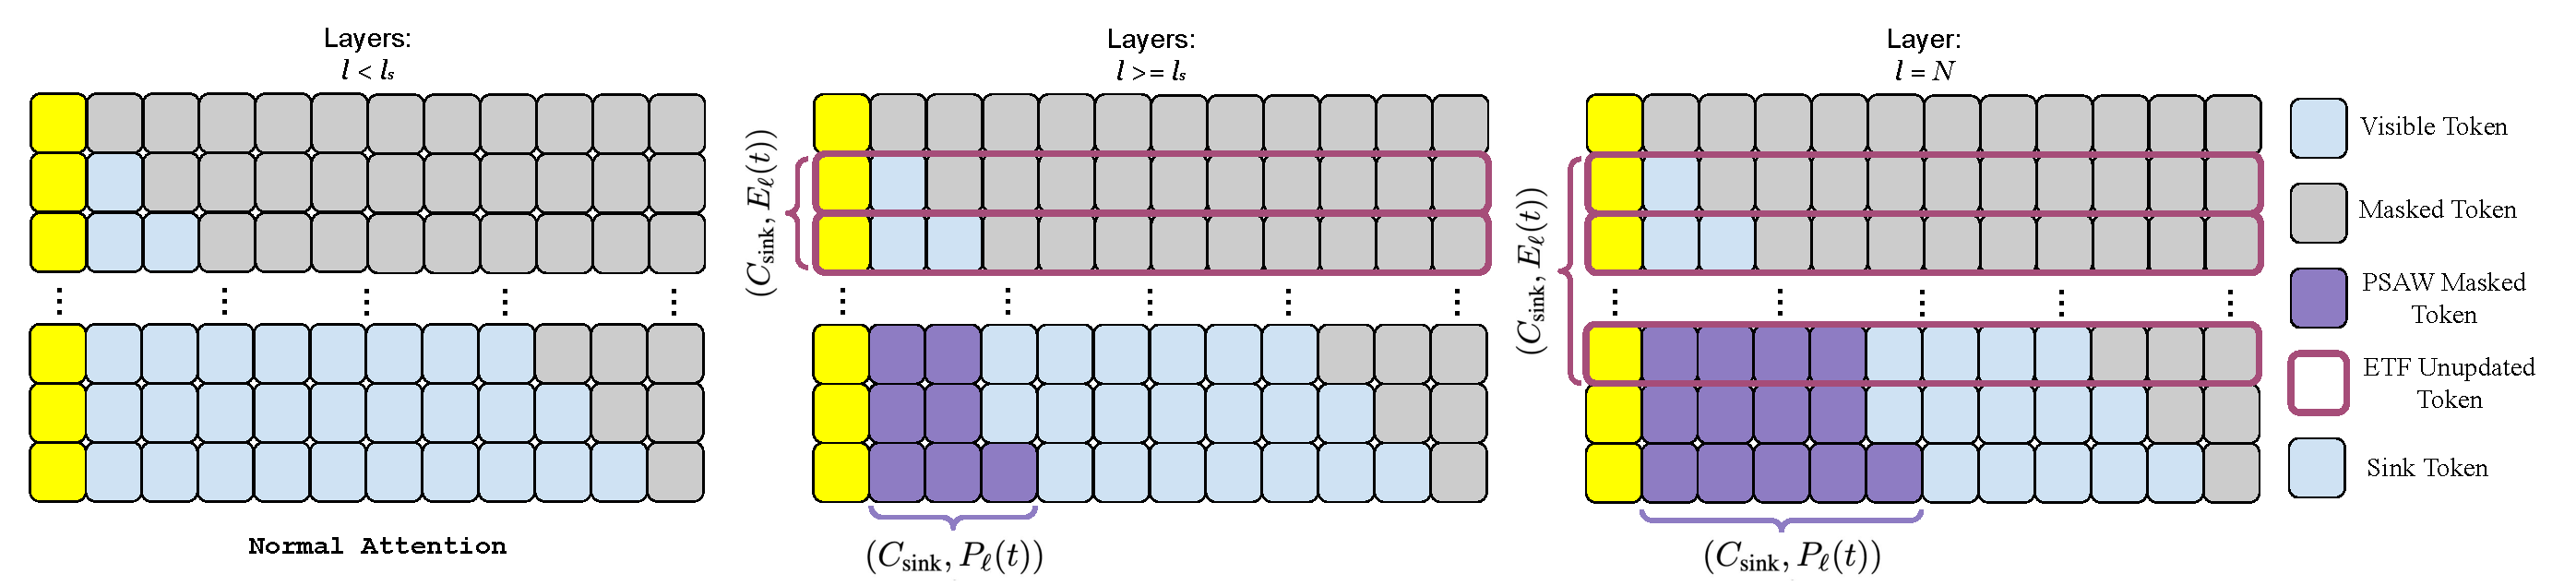
\includegraphics[width=0.95\linewidth]{assets/PSAW-ETF.pdf}
\centering
%\vspace{-0.5em}
    \caption{\textbf{Visual illustration of PSAW and ETF in prefill stage.} When $\ell<\ell_s$, attention is unchanged. For $\ell\ge\ell_s$, both methods prune redundant computation: \textbf{PSAW} computes a per-step sliding window, so the set of \textcolor{PSAW}{masked tokens} can vary across steps (columns); \textbf{ETF} applies a fixed prune range and freezes \textcolor{ETF}{earlier tokens} so they no longer update.}
    \label{fig:psaw&etf}
    \vspace{-0.5em}
\end{figure*}
%------------------------------------------------------


\subsection{Progressive Sliding Attention Window}
\label{sec:psaw}
% \subsubsection{Progressive Sliding Attention Window}

PSAW progressively narrows each layer’s attention window \textbf{during both prefill and decoding}. Consistent with \textbf{Observation~2}, attention is largely localized~\cite{zhang2023h2o,wan2024d2o}: apart from sink tokens, very early tokens receive negligible mass from later queries, and their content has already been propagated forward in lower layers. Thus, attending to them again in deeper layers is redundant.



Let $P_{\ell}(t)$ denote the earliest visible (non-sink) position at step $t$ for layer $\ell$, and let $N$ be the total number of layer. We mask tokens in the index range $(C_{\text{sink}},P_{\ell}(t))$, making the visible set $\{1,\ldots, C_{\text{sink}}\}\cup \{P_{\ell}(t),\ldots,t\}$. Let $\ell_s$ be the layer depth at which pruning starts, we define
\begin{equation}
\label{eq:psaw}
P_\ell(t)=
\begin{cases}
0, &\ell < \ell_s
\\
\big\lfloor (1 \!-\!\phi\;^{\alpha\cdot\frac{\ell-\ell_s}{N-\ell_s}}) \, t \big\rfloor, &\ell \ge \ell_s
\end{cases}
%\;\; \text{where} \;\; \alpha \ge 1 
\end{equation}
where $\phi\!\in\!(0,1)$ and $\alpha\!\ge\!0$. For $\ell\!<\!\ell_s$, no pruning is applied to preserve early-information propagation. For $\ell \!\ge\! \ell_s$, the boundary $P_\ell(t)$ moves monotonically forward with depth because $\phi^{\,\alpha\cdot\frac{\ell-\ell_s}{N-\ell_s}}$ decreases as $\ell$ increases, yielding a progressively shrinking window. We adopt an exponentially decaying schedule rather than a linear one to better match attention locality biases, e.g., positional long-term decay~\cite{su2024roformer} and softmax concentration, yielding tighter alignment with the empirical attention drop in long-range influence across layers (see \textbf{Appendix B}). The parameter $\alpha$ controls the decay schedule, while $\phi^\alpha$ sets the top-layer truncation strength. A visualization of the PSAW mask is shown in Fig.~\ref{fig:psaw&etf}, where \textcolor{PSAW}{tokens in soft violet} indicate masked tokens. 

Theoretically, by assuming attention probability mass with an exponential recency schedule beyond sink tokens, PSAW achieves a design-time certificate $\beta_{\mathrm{th}}^{\mathrm{PSAW}}$ and a tightened MI bound that improves as $\phi^\alpha$ decreases or $\lambda_\ell$ grows.



\subsection{Early Token Freezing}
\label{sec:etf}
During \textbf{prefill}, ETF reduces computation by freezing an expanding prefix of early tokens in deeper layers. The intuition is that information from early tokens has already been propagated forward in shallower layers; further updating them yields diminishing returns. This implementation is also supported by the cross-layer redundancy (Sec.~\ref{sec:intro})~\cite{liu2405minicache}. Let $E_\ell(t)$ denote the last frozen (non-sink) index at layer $\ell$ and step $t$. Tokens with positions in $(C_{\text{sink}},E_\ell(t))$ are excluded from updates: they reuse their previous-layer hidden states, and their attention computations are skipped. Analogous to PSAW, we define
\begin{equation}
\label{eq:etf}
E_\ell(t)=
\begin{cases}
0, &\ell < \ell_s
\\
\big\lfloor (1 \!-\!\psi\;^{\gamma \cdot\frac{\ell-\ell_s}{N-\ell_s}}) \, t \big\rfloor, &\ell \ge \ell_s
\end{cases}
\end{equation}
where $\psi\!\in\!(0,1)$ controls the final unfrozen fraction, and $\gamma\!>\!0$ modulates the nonlinearity of the schedule. A visualization is provided in Fig.~\ref{fig:psaw&etf}, where \textcolor{ETF}{tokens with reddish-purple edges} are frozen. Aligning PSAW, giving a small, depth-decaying budget $\beta_{\mathrm{th}}^{\mathrm{ETF}}$ and a correspondingly tight MI bound, ETF achieves a design-time guarantee by increasing $\ell_s$ or $\mu$, as detailed in \textbf{Appendix D}.


%------------------------------------------------------
\begin{figure}[!t]

\includegraphics[width=0.45\textwidth]{assets/parallel.pdf}
\centering
%\vspace{-1em}
    \caption{\textbf{Parallel CPE acceleration.} \emph{Top:} sequential baseline. \emph{Bottom:} parallel design that fuses index manipulation with attention and directly computes TSA scoring for shared heads. \textcolor{ETF}{ETF masking} will be omitted in decoding.}
    \label{fig:parallel}
    \vspace{-0.5em}
\end{figure}
%--------


\subsection{Parallel Acceleration}

\paragraph{Sequential execution} During inference, CPE executes TSA components in the order shown in Fig.~\ref{fig:parallel} (Top). After KV projection (Eq.~\eqref{eq:qkv-proj}), %\textit{ETF} freezes updates of early tokens (ETF masking is omitted during decoding). 
\textit{ETF} freezes early tokens from further updates; during decoding, explicit ETF masking is unnecessary because only the newly generated position is updated.
Next, \textit{CIS} computes critical sets for shared heads using cosine gating and neighbor dilation (Eqs.~\eqref{eq:cos_sim} and \eqref{eq:neighboring}). We then perform full scoring and build the \textit{PSAW} mask for redundant-attention pruning. For heads that still require retrieval, the top-$k$ oracle is applied to obtain their critical sets. Finally, masks are applied so that each head attends only to its critical set.


\paragraph{Parallel acceleration} Many steps depend only on known quantities and can be prepared or executed in parallel (Fig.~\ref{fig:parallel} (Bottom)). Specifically, previously computed critical sets are cached, and the PSAW mask is query-independent, allowing pre-computation. For CIS-shared heads, critical sets are already known, so full scoring is skipped and we compute attention only over valid indices (TSA scoring). Operations for shared heads and retrieval heads run concurrently, and the overall latency is determined by the slower branch.








\section{Experiments}

\begin{table}[t]
\centering
%\footnotesize
\scriptsize
\caption{\textbf{Evaluation of different methods on GSM8K and COQA.} The best result (excluding origin) in each column is highlighted in bold. Comp* refers to the theoretical time complexity for each method to select critical KV cache tokens, where $\mathcal{O}(1)$ denotes constant time complexity, and $T$ represents the theoretical computation time for a dense attention mechanism.}
\label{tab:gsm_coqa}
\begin{tabular}{l|l|cccccc}
\toprule
Model & Method & $\hat{\rho}$ & GSM8K $\uparrow$ & COQA $\uparrow$ & Comp* $\downarrow$ \\
\midrule
\multirow{12}{*}{\shortstack{LLaMA2\\-7b-chat}}
& Original  & -  & 0.2297/0.2297 & 0.5997 & - \\
& H2O \cite{zhang2023h2o}   & -        & 0.0986/0.0144 & 0.4952 & $\mathcal{O}(1)$ \\
& Quest \cite{tang2406quest}  & -       & 0.0478/0.0462 & 0.5713 & 0.1250$T$ \\
& DS \cite{yang2024post}  & -   & 0.1713/0.1706 & 0.5978 & 0.0625$T$ \\
\cmidrule{2-6}
& Hshare-1 \cite{wuhshare} & 0.281  & 0.1803/0.1703 & 0.5898 & 0.0180$T$ \\
& Hshare-2 \cite{wuhshare} & 0.125   & 0.1524/0.1145 & 0.5672 & 0.0080$T$ \\
\cmidrule{2-6}
& \multirow{3}{*}{CIS (ours)}  & 0.164  & \textbf{0.1842}/\textbf{0.1827} & 0.6085 & 0.0104$T$ \\
&  & 0.087   & 0.1804/0.1782 & 0.6072 & 0.0055$T$ \\
&  & \textbf{0.062}   & 0.1759/0.1751 & 0.6068 & \textbf{0.0039}$T$ \\
\cmidrule{2-6}
& \multirow{3}{*}{CIS$^\ast$ (ours)}  & 0.161  & 0.1812/0.1804 & \textbf{0.6063} & 0.0103$T$ \\
&  & 0.084   & 0.1789/0.1782 & 0.6063 & 0.0047$T$ \\
&  & 0.063   & 0.1736/0.1729 & 0.6083 & 0.0040$T$ \\
\midrule
\multirow{10}{*}{\shortstack{LLaMA3\\-70b}} 
& Original  & -   & 0.8067/0.8052 & 0.7085 & - \\
& DS \cite{yang2024post}   & - & 0.7415/0.7392 & 0.7045 & 0.0625$T$ \\
\cmidrule{2-6}
& Hshare-1 \cite{wuhshare} & 0.281  & 0.7512/0.7437 & 0.7010 & 0.0180$T$ \\
& Hshare-2 \cite{wuhshare} & 0.125   & 0.7415/0.7346 & 0.6960 & 0.0080$T$ \\
\cmidrule{2-6}
& \multirow{3}{*}{CIS (ours)}  & 0.183  & \textbf{0.7613/0.7592} & 0.7045 & 0.0117$T$ \\
&  & 0.082   & 0.7553/0.7526 & 0.7021 & 0.0052$T$ \\
&  & 0.064   & 0.7528/0.7511 & 0.7003 & 0.0041$T$ \\
\cmidrule{2-6}
& \multirow{3}{*}{CIS$^\ast$ (ours)}  & 0.179  & 0.7584/0.7556 & \textbf{0.7068} & 0.0114$T$ \\
&  & 0.079   & 0.7542/0.7527 & 0.7003 & 0.0050$T$ \\
&  & \textbf{0.061}   & 0.7536/0.7504 & 0.7001 & \textbf{0.0038}$T$ \\
\midrule
\multirow{10}{*}{\shortstack{Mistral\\-7b}} 
& Original & -   & 0.3821/0.3813 & 0.6758 & - \\
& DS \cite{yang2024post} & -  & 0.3262/0.3227 & 0.6693 & 0.0625$T$ \\
\cmidrule{2-6}
& Hshare-1 \cite{wuhshare} & 0.281   & 0.3199/0.3154 & 0.6560 & 0.0180$T$ \\
& Hshare-2 \cite{wuhshare} & 0.125   & 0.2818/0.2684 & 0.6387 & 0.0080$T$ \\
\cmidrule{2-6}
& \multirow{3}{*}{CIS (ours)} & 0.194  & \textbf{0.3325/0.3302} & 0.6703 & 0.0124$T$ \\
&  & 0.088   & 0.3281/0.3275 & 0.6684 & 0.0056$T$ \\
&  & \textbf{0.065}   & 0.3233/0.3201 & 0.6710 & \textbf{0.0041}$T$ \\
\cmidrule{2-6}
& \multirow{3}{*}{CIS$^\ast$ (ours)} & 0.189  & 0.3292/0.3257 & 0.6691 & 0.0121$T$ \\
&  & 0.091   & 0.3216/0.3204 & 0.6714 & 0.0058$T$ \\
&  & 0.068   & 0.3204/0.3175 & \textbf{0.6754} & 0.0043$T$ \\
\bottomrule
\end{tabular}
\end{table}


\subsection{Experimental Setup}

We evaluate our CPE on two widely-used model families: LLaMA~\cite{touvron2023llama} and Mistral~\cite{jiang2023mistral7b}. Specifically, we select LLaMA2-7B-Chat, LLaMA3-70B, and Mistral-7B for our experiments. As baselines, we select one TDO method H2O~\cite{zhang2023h2o}, two QAA algorithms: Quest~\cite{tang2406quest} and DS~\cite{yang2024post}, as well as a SOTA retrieval-based PoHS instantiation: HShare~\cite{wuhshare}. We report results on GSM8K~\cite{cobbe2021gsm8k}, COQA~\cite{reddy2019coqa}, and LongBench~\cite{bai2023longbench}.


In our CPE, we adopt the following default hyperparameters. For CIS, we set the similarity threshold $\tau\!=\!0.8$, and apply dilation on the $m \!=\! \lfloor k/3\rfloor$ highest-score indices with radius $r=1$. Pruning and freezing of PSAW and ETF start from $\ell_s \!=\! \lfloor 3N/4 \rfloor$ for a model with $N$ layers. PSAW uses $\phi \!=\! 0.7$ and $\alpha \!=\! 1$, while ETF uses $\psi \!=\! 0.5$ and $\gamma \!=\! 1$. 

Because CIS performs head-level KV sharing to avoid full retrieval, we define the \emph{per-step retrieval ratio} $\rho_t\!=\!\frac{R_t}{H\cdot N}$ to measure the retrieval frequency, where $R_t$ is the number of performed head–layer retrieval at step $t$, and $H\cdot N$ is the amount required by a naïve top-$k$ oracle. The ratio $\rho_t$ is controlled by the CIS block size $s$ and the similarity threshold $\tau$. In reports, we present the averaged ratio $\hat{\rho}=\tfrac{1}{T}\sum^{T}\rho_t$ over the $T$ generation steps. 


\subsection{Results on GSM8K and COQA}
\label{sec:gsm8k&coqa}

%\paragraph{Datasets and Metrics}
\subsubsection{Datasets and Metrics}
We perform zero-shot evaluation with LM-Eval on the GSM8K~\cite{cobbe2021gsm8k} and COQA~\cite{reddy2019coqa} benchmarks. GSM8K comprises roughly 8 000 grade-school mathematics problems, whereas COQA targets multi-turn conversational question answering. The mean input lengths are about 500 tokens (GSM8K) and 2 000 tokens (COQA). Following prior work, we report both flexible and strict exact-match (EM) accuracy on GSM8K, and EM on COQA.

%\paragraph{Inference Details}
\subsubsection{Inference Details}
We apply TSA in the decoding stage and solely evaluate CIS as presented in Table~\ref{tab:gsm_coqa}. We select a critical KV budget $C_t \!=\! 128$ ~\cite{wuhshare}. For CIS and Hshare, we set $C_{\text{local}} \!=\! 32$, and $k \!=\! 88$ in the middle. Since CIS dilation incurs additional KV budget during sharing, we therefore additionally include a variant CIS$^\ast$, which sets $k=72$, yielding its average budget close to 128. We choose $s\in\{8,16,20\}$ to vary $\hat{\rho}$.



\begin{table*}[t]

\footnotesize
\centering
\caption{\textbf{Evaluation of different methods on sixteen English datasets in Longbench} and the best result in each row (excluding the original) is highlighted in bold. Here, the retrieval complexity of H2O, Quest, DS, and HShare is just the same with Table~\ref{tab:gsm_coqa}.}
\label{tab:longbench}
\begin{tabular}{lcccc|cc|cc|cc|cc}
\toprule
\multicolumn{1}{c}{\multirow{2}{*}{\textbf{Dataset}}} & \multicolumn{12}{c}{\textbf{Method}} \\
\cmidrule(lr){2-13}
 & Original & H2O \cite{zhang2023h2o} & Quest \cite{tang2406quest} & DS \cite{yang2024post} & \multicolumn{2}{c|}{HShare \cite{wuhshare}}  & \multicolumn{2}{c|}{CIS (ours)} & \multicolumn{2}{c|}{CIS$^\ast$ (ours)} & \multicolumn{2}{c}{CPE (ours)}\\
\midrule

$\hat{\rho}$ & - & - & - & - & 0.281 & 0.125 & 0.177 & 0.083 & 0.164 & 0.085 & 0.174 & 0.079\\

\midrule

MultiNews   & 26.22 & 24.88 & \textbf{26.49} & 26.30 & 26.05 & 25.22 & 26.47 & 25.98 & 26.18 & 26.40 & 26.11 & 26.02\\
Musique            & 8.65  & 6.24  & 4.62 & 8.72  & 8.42  & 8.09 & 8.47 & 6.98 & 8.74 & 8.68 & 8.69 & 7.50\\
HotpotQA  & 27.72 & 27.58 & 21.94 & 27.44 & 27.32 & \textbf{29.13} & 27.54 & 28.64 & 26.72 & 27.60 & 27.39 & 27.10\\
Qasper & 21.88 & 17.32 & 16.96 & 20.98 & 20.12 & 19.60 & 21.24 & 21.18 & 20.87 & 20.79 & 20.94 & \textbf{21.63}\\
2WikiMQA  & 31.18 & 31.38 & 29.42 & 32.01 & 31.46 & 31.43 & \textbf{32.51} & 30.78 & 30.05 & 30.70 & 29.06 & 31.15\\
Repo-P & 52.14 & \textbf{51.81} & 50.24 & 48.44 & 50.79 & 51.63 & 50.99 & 50.03 & 50.65 & 50.88 & 51.64 & 51.12\\
TriviaQA  & 83.09 & 81.90 & 82.42 & 83.23 & \textbf{83.91} & 82.16 & 79.57 & 81.46 & 81.04 & 79.76 & 79.78 & 81.35\\
Trec   & 64.5  & 62.5  & 64.0 & 61.05 & 60.5  & 58.5 & 62.5 & 63.5 & 64.5 & 62.5 & \textbf{65.0} & 62.0\\
Qmsum   & 20.91 & 20.74 & \textbf{21.36} & 20.75 & 20.59 & 20.74 & 20.53 & 20.93 & 20.98 & 20.92 & 20.78 & 20.66\\
NarrativeQA  & 18.83 & 17.01 & \textbf{18.21} & 17.54 & 17.31 & 17.31 & 17.90 & 17.05 & 17.65 & 16.30 & 16.55 & 17.96\\
GovReport   & 26.55 & 23.45 & 25.46 & \textbf{27.04} & 25.85 & 25.85 & 26.63 & 26.39 & 26.07 & 26.39 & 25.63 & 25.78\\
LCC    & 58.26 & 56.55 & \textbf{56.74} & 54.87 & 56.23 & 56.11 & 55.35 & 54.43 & 54.89 & 55.10 & 55.62 & 54.22\\
PC      & 2.77  & 1.87  & 2.33 & 3.15 & 2.30  & 2.30 & 2.69 & 3.12 & 2.38 & \textbf{3.34} & 3.27 & 1.93\\

Samsum  & 41.01 & 40.18 & 40.91 & \textbf{41.30} & 39.77 & 40.02 & 40.96 & 40.52 & 39.04 & 39.68 & 40.11 & 40.19\\
PR-EN & 6.5 & 5.0   & 6.5  & 6.0  & 6.0   & 6.0 & 8.5 & 7.0 & 6.0 & \textbf{9.5} & 6.0 & 6.0\\
MQA-EN    & 36.15 & 33.64 & 31.99 & 35.83 & 34.08 & 32.37 & 36.64 & 36.54 & 37.29 & 37.06 & 37.47 & \textbf{37.96}\\
\midrule
Average   & 32.90 & 31.38 & 31.35 & 32.11 & 31.97 & 31.49 & \textbf{32.40} & 32.15 & 32.06 & 32.22 & 32.11 & 32.02\\
\bottomrule
\end{tabular}
\end{table*}


%------------------------------------------------------
\begin{figure}[!t]
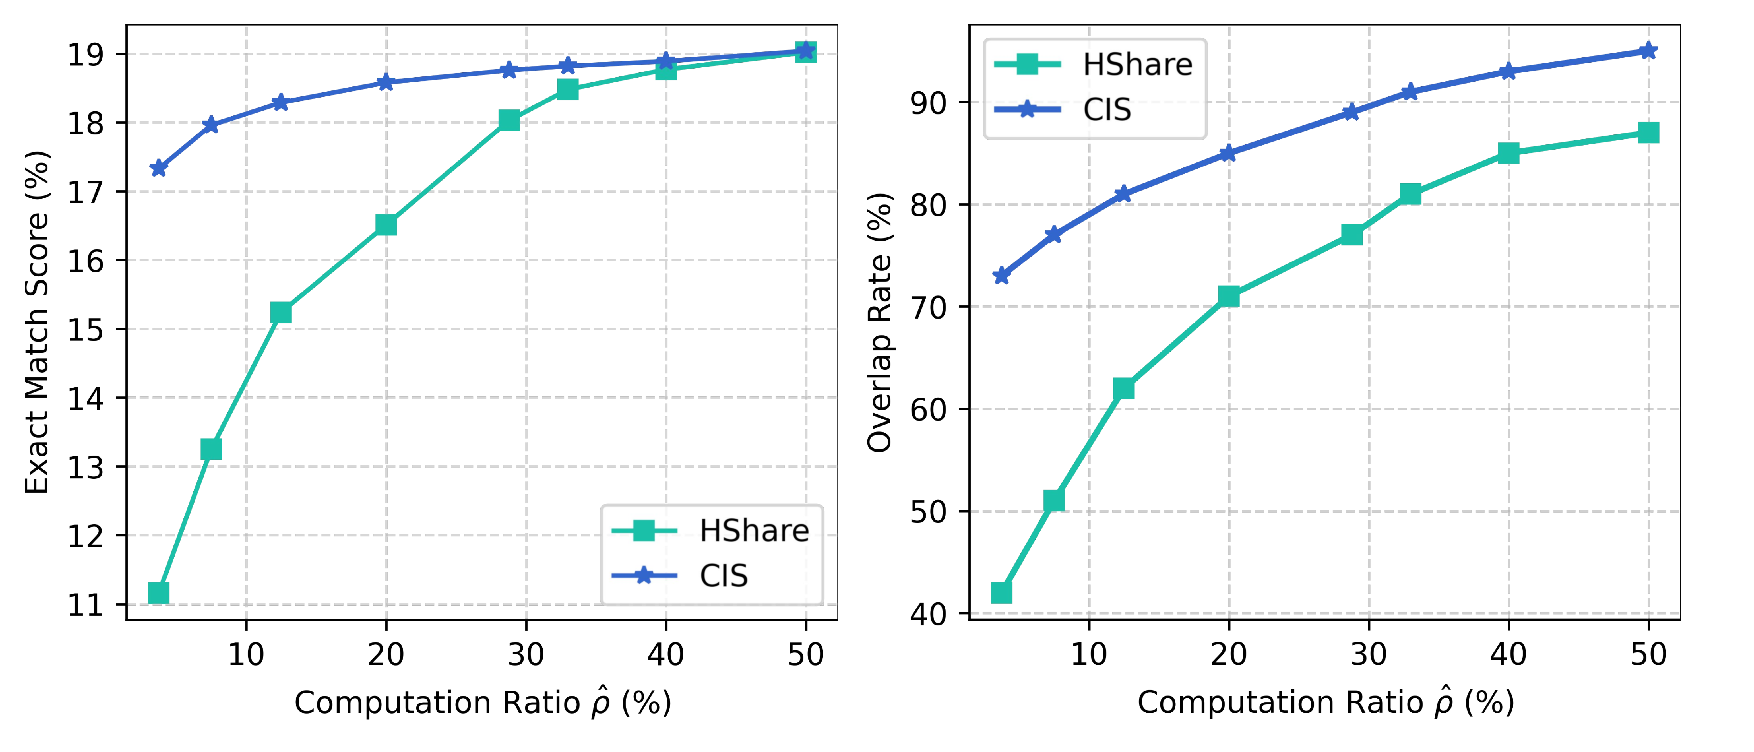
\includegraphics[width=0.48\textwidth]{assets/cis-vs-hshare.pdf}
\centering
\vspace{-1em}
    \caption{\textbf{CIS vs. HShare on GSM8K across computation ratios.} \emph{Left}: Exact-match score accuracy comparisons. \emph{Right}: Overlap comparisons between each method’s retrieved critical set and the top-$k$ oracle.}
    \label{fig:cis_vs_hshare}
    %\vspace{-1.5em}
\end{figure}
%--------

%\paragraph{Result Analysis}
\subsubsection{Result Analysis}


As shown in Table~\ref{tab:gsm_coqa}, CIS and its budget-matched variant CIS$^\ast$ consistently deliver a superior accuracy–efficiency trade-off to PoHS baselines on GSM8K and COQA. On LLaMA-2-7B-Chat, CIS at low selection cost already surpasses SOTA HShare, i.e., $40$–$55\%$ lower complexity at higher accuracy. The advantage widens on LLaMA-3-70B with deeper layers, consistent with reduced cross-layer error accumulation under sharing. CIS$^\ast$ still outperforms HShare at matched budgets, isolating selection \emph{quality} rather than capacity as the driver of the gains. Efficiency is materially better. For instance, on LLaMA-3-70B, CIS uses $0.0052T$ selection cost versus DS’s $0.0625T$.


To further evaluate the accuracy-efficiency trade-offs of CIS, we compare the results of HShare and CIS under different computation ratios on GSM8K. As shown in Fig.~\ref{fig:cis_vs_hshare}(left), when computation ratio is below 30\%, the performance of HShare degrades sharply, while CIS maintains high accuracy. From the perspective of retrained attention mass, Fig.~\ref{fig:cis_vs_hshare}(right) shows that the average overlap of HShare collapses at low computation ratio. These results further demonstrate that the selection quality of CIS is much better than HShare under aggressive sharing.

% As shown in Tab.~\ref{tab:gsm_coqa}, CIS and its budget-matched variant CIS$^\ast$ consistently deliver a superior accuracy–efficiency trade-off to PoHS baselines on GSM8K and COQA. On LLaMA-2-7B-Chat, CIS at low selection cost already surpasses SOTA HShare: CIS attains $0.1842/0.1827$ (flex/strict) with selection cost $0.0104T$, versus HShare(3/4-3/4-1/2) at $0.1803/0.1703$ and $0.0180T$, i.e., $40$–$55\%$ lower complexity at higher accuracy. These gains indicate that CIS under PrHS tightly controls induced error. CIS also shows strong strict–flex robustness on GSM8K (only $0.1842\!\to\!0.1827$ across various computation ratios), whereas HShare drops from $0.1803$ to $0.1703$, suggesting genuine reasoning accuracy rather than formatting artifacts. The advantage widens on LLaMA-3-70B with deeper layers, consistent with reduced cross-layer error accumulation under sharing.

% CIS$^\ast$ still outperforms HShare at matched budgets, isolating selection \emph{quality} rather than capacity as the driver of the gains. Efficiency is materially better: on LLaMA-3-70B, CIS uses $0.0052T$ selection cost versus DS’s $0.0625T$, and across settings CIS operates at $0.0041$–$0.0117T$ compared to HShare’s $0.0180T$, sharpening the accuracy–efficiency frontier. Even under extreme sharing ($\hat{\rho}\!\approx\!0.06$–$0.08$), CIS remains competitive. On COQA, CIS and CIS$^\ast$ are near-dense or better—$0.6103$ on LLaMA-2-7B-Chat exceeds dense $0.5997$, and $0.7068$ on LLaMA-3-70B is close to $0.7085$—indicating that conversational understanding is well preserved.

% To further evaluate the accuracy-efficiency trade-offs of CIS, we compare the results of HShare and CIS under different computation ratios on GSM8K. Fig.~\ref{fig:cis_vs_hshare}(left) plots the EM-computation curve. When computation ratio is high, the accuracy gap between CIS and HShare~\cite{wuhshare} remains relatively small. Below 30\%, the performance of HShare degrades sharply, while CIS maintains high accuracy. From the perspective of retrained attention mass, Fig.~\ref{fig:cis_vs_hshare}(right) shows the average overlap of the true positive of retrieved critical set compared to top-k oracle. Similar to EM, HShare’s overlap rate collapses at low computation ratio. Inspection reveals that HShare's coarse sharing schedules propagate indices between queries with low semantic similarity. Moreover, even for heads with high semantic similarity, its shared set is fragmented (Fig.~\ref{fig:index-frag}), missing many true positives. These problems drastically reduces its recall. CIS, by contrast, maintains a much higher overlap rate even under aggressive sharing.


\subsection{Longbench}
\label{sec:longbench}

%\paragraph{Datasets and Metrics}
\subsubsection{Datasets and Metrics}
LongBench contains sixteen English tasks spanning code completion, few-shot learning, document-level QA, summarisation, and synthetic reasoning. We adhere to the official evaluation protocol: MultiNews, Qmsum, GovReport, Samsum with rouge score; Musique, HotpotQA, Qasper, 2WikiMQA, TriviaQA, NarrativeQA, MultifieldQA-EN (MQA) with F1 score; trec with classification accuracy; Passage-Count (PC), Passage-Retrieval-EN (PR-EN) exact-match accuracy; RepoBench-P (Repo-P) and LCC with similarity score.


\begin{table*}[t]
\centering
\caption{Attention operator latency (ms $\downarrow$) of different methods across various batch sizes and sequence lengths. Lower values indicate better performance. HShare-0 corresponds to HShare(3/4-3/4-1/2), and HShare-1 to HShare(1/2-1/2-1/2). The number following each of our methods indicates the block size $s$ used in CIS.}
\label{tab:attention_latency}
\begin{tabular}{cccccccc|cccc}
\toprule
BS & Seqlen & Flash & H2O \cite{zhang2023h2o} & Quest \cite{tang2406quest} & DS \cite{yang2024post} & HShare-0 \cite{wuhshare} & HShare-1 \cite{wuhshare} & CIS-8 & CIS-16 & CPE-8 & CPE-16 \\
\midrule
\multirow{3}{*}{8}
  & 1k & 0.230 & 0.088 & 0.200 & 0.141 & 0.124 & 0.090 & 0.116 & 0.083 & 0.092 & \textbf{0.078}\\
  & 2k & 0.830 & \textbf{0.093} & 0.460 & 0.241 & 0.160 & 0.120 & 0.147 & 0.106 & 0.144 & 0.095 \\
  & 4k & 1.630 & 0.470 & 0.850 & 0.733 & 0.570 & 0.530 & 0.534 & 0.501 & 0.506 & \textbf{0.469} \\
\midrule
\multirow{3}{*}{16}
  & 1k & 0.440 & 0.089 & 0.280 & 0.233 & 0.120 & 0.093 & 0.113 & 0.081 & 0.089 & \textbf{0.075} \\
  & 2k & 1.630 & \textbf{0.110} & 0.770 & 0.422 & 0.230 & 0.190 & 0.214 & 0.178 & 0.196 & 0.165 \\
  & 4k & 3.230 & 0.850 & 2.21  & 1.350 & 1.041 & 0.990 & 0.953 & 0.869 & 0.904 & \textbf{0.821} \\
\bottomrule
\end{tabular}
\end{table*}



\subsubsection{Inference Details}

All baselines apply TSA only during decoding and retain a $512$ KV budget, with a sparsity ratio of ${\approx}$1/8. For HShare and CIS we set $C_{\text{sink}}{=}16$, $C_{\text{local}}{=}64$, and $k{=}432$. With CIS’s neighbor dilation, the effective shared-head set averages $547.5$ tokens. To enable a budget-matched comparison, CIS$^\ast$ reduces the middle-budget to $k{=}388$, equalizing the average KV budget processed during decoding to $512$. For the combined system \textbf{CPE}, we use $k{=}432$ and also activate PSAW and ETF during \emph{prefill}. Reductions achieved in prefill are not counted toward the decoding-budget metric, so CPE further lowers prefill cost in addition to the standard decoding-only comparison. We use block size $s\in\{8,16\}$.

%\paragraph{Results Analysis}
\subsubsection{Results Analysis}

Across sparse baselines, CIS attains the best average while using substantially lower retrieval than SOTA HShare, as shown in Table \ref{tab:longbench}. Specifically, CIS achieves the highest non-dense average, $32.40$, at a moderate retrieval ratio $\hat{\rho}{=}0.177$, surpassing HShare’s best $31.97$ at $\hat{\rho}{=}0.281$ with $37\%$ less retrieval. Moreover, CIS$^{\ast}$ remains competitive with HShare while substantially reducing retrieval, indicating that gains stem from selection quality rather than capacity. CPE preserves this competitiveness ($32.11$) while additionally reducing prefill cost. Although prefill reductions are not counted in the decoding budget, CPE still ties or wins on several tasks, showing that pruning and freezing early tokens remove redundant compute without harming downstream reasoning—consistent with the error control guaranteed by PrHS.

% Across sparse baselines, CIS attains the best average while using substantially lower retrieval than SOTA HShare, as shown in Table \ref{tab:longbench}. Specifically, CIS achieves the highest non-dense average, $32.40$, at a moderate retrieval ratio $\hat{\rho}{=}0.177$, surpassing HShare’s best $31.97$ at $\hat{\rho}{=}0.281$ with $37\%$ less retrieval. CIS$^{\ast}$ at $\hat{\rho}\!\approx\!0.085$ remains competitive at $32.22$, matching or exceeding HShare at $\hat{\rho}{=}0.125$ while reducing retrieval by $32\%$, indicating that gains stem from selection quality rather than capacity. CPE preserves this competitiveness ($32.11$) while additionally reducing prefill cost.

% CIS yields the strongest non-dense results on retrieval-sensitive tasks. It leads on \textsc{2WikiMQA} ($32.51$), and CIS$^{\ast}$ wins on \textsc{PR-EN} ($9.50$) and \textsc{PC} ($3.34$). These gains align with cosine-gated head sharing plus light neighbor dilation, which improves true-positive recall without inflating the processed KV budget. Performance degrades gracefully as retrieval tightens: reducing $\hat{\rho}$ from $0.177$ (CIS) to $\approx 0.085$ (CIS$^{\ast}$) changes the average by only $0.18$, suggesting stable sharing decisions.

% Although prefill reductions are not counted in the decoding budget, CPE still ties or wins on several tasks (\textsc{TREC} $65.0$, \textsc{MQA-EN} $37.96$, \textsc{Qasper} $21.63$), showing that pruning and freezing early tokens remove redundant compute without harming downstream reasoning—consistent with the error control guaranteed by PrHS.


\begin{table*}[t]
\centering
\caption{Throughput ($\uparrow$) of different methods across various batch sizes and sequence lengths. HShare-0 corresponds to HShare(3/4-3/4-1/2), and HShare-1 to HShare(1/2-1/2-1/2). The number following each of our methods indicates the block size $s$ used in CIS.}
\label{tab:throughput}
\begin{tabular}{cccccccc|cccc}
\toprule
BS & Seqlen & GPT-Fast & H2O \cite{zhang2023h2o} & Quest \cite{tang2406quest} & DS \cite{yang2024post} & HShare-0 \cite{wuhshare} & HShare-1 \cite{wuhshare} & CIS-8 & CIS-16 & CPE-8 & CPE-16 \\
\midrule
\multirow{3}{*}{8}
  & 1k & 228 & 240 & 228 & 228 & 231 & 235 & 233 & 236  & 238 & \textbf{244} \\
  & 2k & 188 & \textbf{234} & 206 & 213 & 222 & 226 & 216 & 224  & 225 & 233 \\
  & 4k & 118 & \textbf{228} & 152 & 201 & 214 & 217 & 216 & 220  & 219 & 227 \\
\midrule
\multirow{3}{*}{16}
  & 1k & 374 & 441 & 410 & 423 & 430 & 439 & 433 & 443 & 441 & \textbf{449} \\
  & 2k & 233 & 416 & 287 & 360 & 398 & 411 & 402 & 415 & 412 & \textbf{421} \\
  & 4k & 136 & \textbf{396} & 175 & 286 & 350 & 365 & 352 & 364 & 362 & 384 \\
\bottomrule
\end{tabular}
\end{table*}



\subsection{Efficiency Evaluation}

\subsubsection{Inference Detail}

Following prior work~\cite{yang2024post,wuhshare}, we measure (i) self-attention operator latency and (ii) end-to-end throughput in the decoding stage. Experiments use \mbox{LLaMA-2-7B-Chat} on a server with an Intel Xeon Platinum 8336C CPU, a single NVIDIA A100 GPU, and 120 GB RAM. For the operator benchmark, FlashAttention-2 (Flash)~\cite{dao2022flashattention} serves as the dense baseline. For the end-to-end benchmark, we use GPT-fast~\cite{pytorch} as the dense baseline and replace its attention module with our TSA implementation. We test batch sizes ${8,16}$ and sequence lengths $1\text{k}$–$4\text{k}$ at a token sparsity ratio of $1/8$. We report results for CIS and CPE (CIS+PSAW; ETF is prefill-only) with block sizes $s\in{8,16}$. Because CIS confines sharing within a block, the extra cache is minimal, and the added per-step bookkeeping is bounded by $\mathcal{O}(H s k)$.

% , we add  as our baseline, which is an optimized dense attention mechanism designed to improve the speed and efficiency and ranks among the fastest attention mechanisms

\subsubsection{Results Analysis}

\paragraph{Operator latency} As shown in Table~\ref{tab:attention_latency}, CPE-16 delivers the fastest kernel at both small and long contexts for each batch size (BS). At $2\text{k}$ tokens and BS$=16$, it attains a $9.9\times$ speedup over Flash. At $4\text{k}$ tokens, relative to the SOTA PoHS baseline, HShare-1, CPE-16 reduces latency by $11.5\%$ (BS$=8$) and $17.1\%$ (BS$=16$), and it outperforms DS by up to $39\%$ at BS$=16$. H2O is competitive at $2\text{k}$, where its ultra-light TDO pattern minimizes overhead. CIS alone also confers a clear advantage: at BS$=16$, CIS-16 is $11$–$15\%$ faster than HShare-1. The pattern is consistent with head-level sharing plus PSAW amortizing their $\mathcal{O}(H s k)$ bookkeeping once the GPU is well utilized, leaving reduced active KV compute as the runtime driver.




\paragraph{End-to-end throughput} Operator gains translate to real decoding speed, as shown in Table~\ref{tab:throughput}. Relative to GPT-Fast, CPE-16 reaches $2.82\times$ at BS$=$16, $4\text{k}$. At BS$=16$ and $1$–$2\text{k}$, CPE-16 achieves the highest throughput, edging out H2O; at BS$=8$, it leads at $1\text{k}$ and effectively ties H2O at longer contexts. As batch size and sequence length grow, the gap between operator-level and end-to-end gains narrows due to non-attention bottlenecks (MLPs, sampling), yet CPE consistently ranks first or near-first across realistic loads, with $s{=}16$ providing the strongest throughput.


\paragraph{Effect of block size} Across settings, $s{=}16$ is consistently faster than $s{=}8$ for both CIS and CPE. Larger boundaries reduce launch and index-management overhead and allow sharing decisions to persist longer, so the small increase in per-block work is negligible compared to better kernel efficiency. This argues for $s{=}16$ as the default in high-throughput deployments.

\definecolor{orange}{HTML}{FF5C33}
\definecolor{darkgreen}{HTML}{2E7D32}

\subsection{Further Analysis}

%------------------------------------------------------
\begin{figure}[!t]
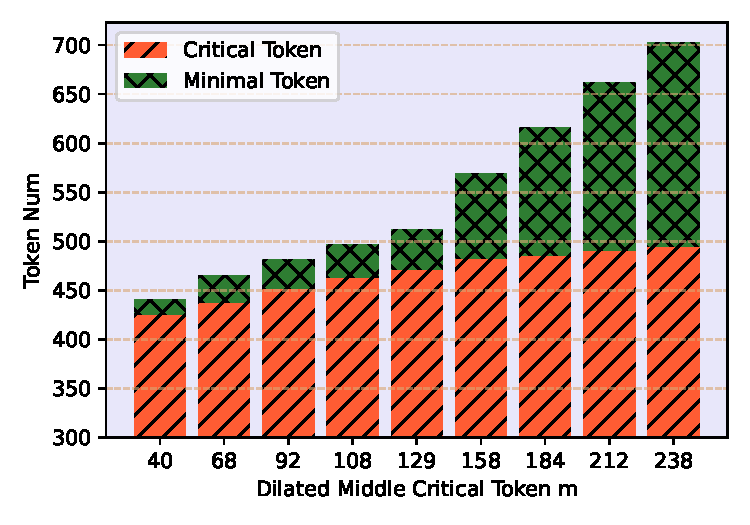
\includegraphics[width=0.4\textwidth]{assets/cis-dilation.pdf}
\centering
\vspace{-1em}
    \caption{\textbf{Effect of CIS dilation on LongBench NarrativeQA.} The stacked bar shows the average processed KV set: the \textcolor{orange}{orange segment} counts tokens that also appear in the top-$k$ oracle (budget 512, following Sec.~\ref{sec:longbench}), while the \textcolor{darkgreen}{green segment} counts minimal tokens not in the top-$k$ set.}
    \label{fig:cis-dilation}
    \vspace{-0.5em}
\end{figure}
%--------

%\paragraph{CIS Expansion}
\subsubsection{CIS Dilation}
\label{sec:cis-dilation}

We assess CIS dilation using the CIS$^\ast$ configurations from Sec.~\ref{sec:longbench}, varying the number of top indices dilated $m$. As shown in Fig.~\ref{fig:cis-dilation}, the number of \emph{additional} tokens beyond the top-$k$ set remains small for moderate $m$; dilation overhead grows gradually as $m$ increases, and the added tokens are predominantly low-importance. Inspecting shared queries explains this behavior as follows. Their most influential critical tokens are tightly clustered and spatially stable, so dilation contributes few extra indices. In contrast, when the budget begins to include low-score tokens, these indices are irregular and scattered, and dilation substantially inflates the set. This motivates restricting dilation to a top fraction of retrieved tokens. In practice, the expanded set also overlaps heavily with the remaining retrieved indices, further limiting redundancy.


\begin{table*}[t]
\centering
\caption{\textbf{Hyperparameter tuning on LLaMA2-Chat-7B for CPE.} The COQA setting for CIS follows the CIS$^\ast$ configuration, and HyperKV follows the HyperKV configuration, as described in Sec.~\ref{sec:gsm8k&coqa}. WikiText perplexity (PPL) is measured only during the prefilling stage. The Avg.Token measures the average processed tokens per head only in the decoding stage.}
\label{tab:hyper-tune}
\begin{tabular}{l|ccccccc|cccccc}
\toprule
Methods & $s$ & $\tau$ & $r$ & $\phi$ & $\psi$ & $\alpha$ & $\gamma$ & $\hat{\rho}$ & Avg. Token & Wiki PPL & GSM8K(flexible) & COQA(EM/F1)\\
\midrule
\multirow{4}{*}{CIS}
  & 4 & 0.8 & 1 & - & - & - & - & 0.301 & 124 & - & 0.1834 & 0.6023 / 0.7632\\
  & 8 & 0.7 & 1 & - & - & - & - & 0.152 & 131 & - & 0.1801 & 0.6090 / 0.7648\\
  & 8 & 0.8 & 2 & - & - & - & - & 0.184 & 167 & - & 0.1653 & 0.6083 / 0.7650\\
  & 32 & 0.8 & 1 & - & - & - & - & 0.0046 & 136 & - & 0.1693 & 0.6080 / 0.7641\\

\midrule

\multirow{2}{*}{PSAW}
  & - & - & - & 0.5 & - & 1 & - & - & - & 6.120 & 0.1896 & 0.5925 / 0.7568\\
  & - & - & - & 0.7 & - & 1.5 & - & - & - & 6.113 & 0.1803 & 0.5938 / 0.7573\\

\midrule

\multirow{2}{*}{ETF}
  & - & - & - & - & 0.5 & - & 1.5 & - & - & 6.162 & 0.1864 & 0.5962 / 0.7563\\
  & - & - & - & - & 0.4 & - & 1 & - & - & 6.156 & 0.1883 & 0.5962 / 0.7537\\

\midrule

\multirow{2}{*}{CPE}
  & 8 & 0.8 & 2 & 0.7 & 0.5 & 1.2 & 1.2 & 0.176 & 166 & 6.148 & 0.1348 & 0.5998 / 0.7591 \\
  & 32 & 0.8 & 1 & 0.7 & 0.5 & 1 & 1 & 0.0044 & 133 & 6.136 & 0.1634 & 0.5965 / 0.7572\\

\bottomrule
\end{tabular}
\end{table*}

%\paragraph{Ablation Studies}
\subsubsection{Hyperparameter Tuning}
\label{sec:hyper-tune}
\paragraph{Setting} We tune the key knobs of our compression pipeline in Table~\ref{tab:hyper-tune}. For \emph{CIS}, we adopt the CIS$^\ast$ configuration from Sec.~\ref{sec:gsm8k&coqa} and vary the block size $s$, similarity threshold $\tau$, and neighbor radius $r$. For \emph{PSAW} and \emph{ETF} in isolation, we apply them on dense attention, fix $\ell_s=\lfloor 3N/4\rfloor$, and control pruning/freezing aggressiveness via $(\phi,\alpha)$ for PSAW and $(\psi,\gamma)$ for ETF; PSAW is active in both prefill and decoding. For \emph{CPE}, we combine all three components, adding PSAW and ETF to CIS under TSA. We report: the averaged computation ratio $\hat{\rho}$, the average processed tokens per head in decoding (Avg.Token), \emph{prefill}-only WikiText perplexity (PPL), and task accuracy on GSM8K (flex) and COQA (EM/F1).

\paragraph{CIS} Varying $(s,\tau,r)$ reveals the accuracy–efficiency trade-off. Smaller $s$ increases retrieval frequency (higher $\hat{\rho}$), whereas enlarging to $s{=}32$ drives the retrieval ratio down to $\hat{\rho}{=}0.0046$ with only a modest GSM8K accuracy drop; COQA remains notably stable across all $s$. At fixed $s{=}8$, increasing the dilation radius to $r{=}2$ substantially enlarges the active set but yields negligible accuracy change on both GSM8K and COQA; inspection shows that the added neighbors often include low-importance tokens, perturbing the attention-mass distribution without benefits. Slightly loosening $\tau$ has little effect on accuracy. Overall, $s$ is the dominant lever for efficiency, while $\tau$ and $r$ offer fine-grained control of recall versus budget.

\paragraph{PSAW} Prefill pruning is gentle on language modeling quality and downstream accuracy. Increasing aggressiveness from $(\phi{=}0.5,\alpha{=}1)$ to $(\phi{=}0.7,\alpha{=}1.5)$ barely changes WikiText PPL, and COQA is essentially unchanged, while GSM8K (flexible match) decreases only slightly.

\paragraph{ETF} Freezing during prefill shows similarly small effects. Adjusting from $(\psi{=}0.5,\gamma{=}1.5)$ to $(\psi{=}0.4,\gamma{=}1)$ yields virtually identical PPL and a tiny trade between GSM8K and COQA. ETF is therefore a stable knob for further prefill savings and slightly milder freezing is a safe default setting.

\paragraph{CPE} Combining CIS with PSAW and ETF preserves efficiency while keeping quality competitive. With aggressive dilation ($r{=}2$), GSM8K dips to $0.1348$. Increasing block size and reducing dilation to $r{=}1$ lowers selection frequency and trims Avg. Token by ${\sim}20\%$, recovering GSM8K to $0.1634$ with COQA nearly unchanged. Overall, CPE performs best with moderate–large blocks, restricted dilation ($r{=}1$), and mild PSAW/ETF schedules.




%------------------------------------------------------------
\begin{table}[tb]
\centering
\footnotesize
%\normalsize
\caption{Variants of CIS on the similarity designs. The model is LlaMA2-7b-chat.}
\label{tab:cis_variant}
%\resizebox{\linewidth}{!}
{
\begin{tabular}{l|c|ccc}
\toprule
Method & $s$ & GSM8K (flexible/strict) & COQA\\ 
\midrule

%\multirow{2}{*}{Query} & 8  & 0.1744 / 0.1736 & 0.6093  \\ 
% & 16  & 0.1668 / 0.1653 & 0.6093 \\ 

% \midrule

\multirow{2}{*}{Key} & 8  & 0.1547 / 0.1482 & 0.5613 \\ 
 & 16  &  0.1405 / 0.1334 & 0.5608  \\ 

\midrule

\multirow{2}{*}{Hidden} &  8 & 0.1303 / 0.1289 & 0.5416  \\ 
 &  16 &  0.1121 / 0.1108 & 0.5214 \\ 

\bottomrule
\end{tabular}
}
\end{table}
%------------------------------------------------------------

%\paragraph{CIS Variant Designs}
\subsubsection{Similarity Ablations} 

We explore alternative similarity metrics for CIS derived from different representations. Concretely, we replace the default cosine similarity between \emph{query} embeddings (Eq.~\ref{eq:cos_sim}) with cosine similarity computed on (i) hidden states $\bx$ and (ii) key embeddings $\bk$, and evaluate under the CIS$^\ast$ configuration in Sec.~\ref{sec:gsm8k&coqa}. As shown in Table~\ref{tab:cis_variant}, both variants reduce accuracy, with the hidden-state metric degrading most. This indicates that the query, key, and hidden-state spaces emphasize distinct semantics; temporal semantic proximity for CIS is best captured in the \emph{query} space, whereas measuring similarity in $\bx$ or $\bk$ misaligns clusters and harms selection quality.


\section{Conclusion}

In this paper, we propose Pre-hoc Sparsity (PrHS) framework, and derive an upper bound on the mutual-information (MI) loss based on the dropped attention mass. By tightening the MI bound towards the top-$k$ oracle, selectors under PrHS can achieve near-oracle KV compression. We propose \textbf{CPE} that instantiate three orthogonal modules under PrHS: \emph{Clustered Indices Sharing} (CIS), \emph{Progressive Sliding Attention Window} (PSAW), and \emph{Early Token Freezing} (ETF). CIS expands the highest-score indices in each shared critical set to its neighbors, achieving high recall and preserving accuracy even at aggressive (${\ge}90\%$) sharing ratios. PSAW and ETF further amplify sparsity by \textbf{masking tokens} that lie outside a dynamically sliding context window and \textbf{freezing tokens} whose updates have converged, thereby eliminating redundant computation with negligible performance loss. %These selectors are parameterized and tighten. 
Extensive evaluations on GSM8K, COQA, and LongBench demonstrate that CPE (i) matches dense baselines in accuracy under high attention sparsity, (ii) reduces retrieval complexity by up to $3\times$ than recent SOTA HShare~\cite{wuhshare} with even better performance, (iii) delivers up to a $9.9\times$ latency speed-up over FlashAttention and a $2.8\times$ throughput gain over GPT-Fast. These results confirm CPE as an effective and broadly applicable solution for efficient long-context inference in LLMs.


% In this paper, we propose HyperKV, which incorporates three key techniques: Clustered Indices Sharing (CIS), Progressive Sliding Attention Window (PSAW), and Early Token Freezing (ETF). CIS improves the retrieval rate of critical tokens by expanding shared critical indices to their neighbors, thereby maintaining strong model accuracy under high sharing ratios. PSAW and ETF enhance attention sparsity with minimal performance loss by eliminating redundant attention computations. We provide formal theoretical analyses to demonstrate the feasibility of these techniques and support their effectiveness through extensive experiments, showing that HyperKV consistently outperforms existing baselines.

% ====== Requires in the preamble ============================================
% \newtheorem{theorem}{Theorem}

% ============================================================================

\section{Unified Information Bounds}
\label{sec:app_uib}
\subsection{Setup}

We consider the minimal unit of the information bound and fix both the layer and the head. Following the softmax attention distribution defined in Sec.~\ref{sec:inference_background} and Eq.~\ref{eq:attn_eq}, for a query $\bq$, with $\bK=[\bk_1,\dots,\bk_L]$ and $\bV=[\bv_1,\dots,\bv_L]$ denote keys/values for a context of length $L$, we introduce the \emph{latent index} random variable
\begin{equation}
    T\in[L],\qquad \mathbb P(T=i\,|\,\bq,\bK)=A_i(\bq),
\end{equation}
and the routed value $\bV_T$ for token-sparse attention. Let $I_{\mathrm{full}}(\bq)$ denote the (per-query) information carried by full attention, for a size-$n$ selector $\mathcal S\subseteq [L]$, the retained attention mass $\tau_{\mathcal S}(\bq)$ and dropped attention mass $\delta_{\mathcal S}$ are defined as:
\begin{equation}
    \tau_{\mathcal S}(\bq)=\sum_{i\in\mathcal S}A_i(\bq),\qquad
\delta_{\mathcal S}(\bq)=1-\tau_{\mathcal S}(\bq).
\end{equation}
Let $\widetilde A_{\mathcal S}(\bq)$ be the truncated/renormalized distribution (follow the normalization of the softmax)
\begin{equation}
    \widetilde A_i(\bq)=
    \begin{cases}
    A_i(q)/\tau_{\mathcal S}(\bq), & i\in\mathcal S,\\[2pt]
    0,& \text{otherwise},
    \end{cases}
    \quad
    T_{\mathcal S}\sim \widetilde A_{\mathcal S}(\bq).
\end{equation}
Denote by $I_{\mathcal S}(\bq)$ the information of the token-sparse channel that keeps indices in $\mathcal S$ and routes $\bV_{T_{\mathcal S}}$. And let $\mathcal S^{*}(\bq)=\operatorname*{Top}_n\!\big(A(\bq)\big)$ be the top-$n$ oracle set with
\begin{equation}
\label{eq:oracle_attn_mass}
    \tau^{*}(\bq)=\tau_{\mathcal S^{*}}(\bq),\qquad \delta^{*}(\bq)=1-\tau^{*}(\bq).
\end{equation}

\begin{remark}[We bound information via the index channel]
By data processing along $(\bK,\bV)\to T\to \bV_T$, it suffices (and is conservative) to control the loss in mutual information induced by truncating $T$; this yields bounds for
$I_{\mathrm{full}}(\bq)-I_{\mathcal S}(\bq)$.
\end{remark}

\subsection{Two universal technical lemmas}
\label{sec:app_tech_lemmas}

\begin{lemma}[Total-variation of truncation]
\label{lem:tv}
For any size-$n$ selector $\mathcal S$,
\begin{equation}
    \big\|A(\cdot\,|\,\bq)-\widetilde A_{\mathcal S}(\cdot\,|\,\bq)\big\|_{\mathrm{TV}}
=\delta_{\mathcal S}(\bq).
\end{equation}

\begin{proof}
Write $P=A(\cdot|\bq)$ and $Q=\widetilde A_{\mathcal S}(\cdot|\bq)$. Then
\begin{align*}
\|P-Q\|_{\mathrm{TV}}
&=\tfrac12\sum_{i=1}^L |P_i-Q_i| \\
&=\tfrac12\Big(\sum_{i\notin\mathcal S} P_i + \sum_{i\in\mathcal S}\big|P_i-P_i/\tau_{\mathcal S}\big|\Big)\\
&=\tfrac12\big(\delta_{\mathcal S}+\delta_{\mathcal S}\big)=\delta_{\mathcal S}.
\end{align*}\end{proof}\end{lemma}

\begin{lemma}[Continuity of mutual information (MI) under TV perturbations]
\label{lem:continuity}
Let $\bX=(\bK,\bV)$ and consider two channels from $\bX$ to an output random variable $\bY \equiv \bV_T$ and $\bY' \equiv \bV_{T_{\mathcal S}}$, where for each $\bx=(\bk,\bv)$, the conditional law $T|\bX=\bx$ is $A(\cdot\,|\,\bq,\bk)$ and
$T_{\mathcal S}|\bX=\bx$ is the truncated/renormalized $\widetilde A_{\mathcal S}(\cdot\,|\,\bq,\bk)$.
Assume the (uniform) total-variation gap
\begin{align}
    \sup_{\bx}\, &\big\| \mathsf P(T\in\cdot\,|\,\bX=x)-\mathsf P(T_{\mathcal S}\in\cdot\,|\,\bX=x)\big\|_{\mathrm{TV}} \nonumber \\
    &=\delta_{\mathcal S}(\bq)\eqqcolon \delta \in[0,1].
\end{align}
Then, for every input law $\mathsf P_\bX$,
\[
\big|I(\bX;\bY)-I(\bX;\bY')\big|
\;\le\;
2\Big[h_{\mathrm b}(\delta)+\delta\log L\Big],
\]
where $I$ is the MI measure, $h_{\mathrm b}$ is the binary entropy function. Consequently,
\[
0\le I_{\mathrm{full}}(\bq)-I_{\mathcal S}(\bq)
\;\le\;
2\Big[h_{\mathrm b}(\delta_{\mathcal S}(\bq))+\delta_{\mathcal S}(\bq)\log L\Big].
\]
\end{lemma}
\begin{proof}
\label{proof:MI_bound}
\textbf{Step 1: Per-$\bx$ support size and induced kernels.}
Fix $\bx=(\bk,\bv)$. The map $t\mapsto \bv_t$ is deterministic (given $\bx$), hence
$\bY|\bX=\bx$ and $\bY'|\bX=\bx$ are obtained by pushing forward the probability mass function (pmfs) $A(\cdot\,|\,\bq,\bk)$ and $\widetilde A_{\mathcal S}(\cdot\,|\,\bq,\bk)$ through a map with image of size at most $L$:
\[
\mathcal \bY_\bx \;=\;\{\bv_1,\dots,\bv_L\},\qquad |\mathcal \bY_\bx|\le L.
\]
Let $W_x$ and $\widetilde W_x$ denote the conditional pmfs of $\bY|\bX=\bx$ and $\bY'|\bX=\bx$,
respectively. Total variation cannot increase under measurable mappings, so
\begin{equation}
\label{eq:tv-per-x}
\|\bW_\bx-\widetilde \bW_\bx\|_{\mathrm{TV}}
\;\le\;
\|A(\cdot\,|\,\bq,\bk)-\widetilde A_{\mathcal S}(\cdot\,|\,\bq,\bk)\|_{\mathrm{TV}}
\;\le\; \delta.
\end{equation}

\textbf{Step 2: Continuity of (conditional) entropy at fixed $x$.}
For pmfs $P,Q$ on a finite alphabet of size $m$ with
$\|P-Q\|_{\mathrm{TV}}\le \varepsilon$, the classical continuity bound for the
Shannon entropy gives
\begin{align}
\label{eq:entro-cont}
|H(P)-H(Q)|
&\;\le\;
h_{\mathrm b}(\varepsilon)+\varepsilon\log(m-1)  \nonumber \\
&\;\le\; 
h_{\mathrm b}(\varepsilon)+\varepsilon\log m .
\end{align}
Applying \eqref{eq:entro-cont} to $(P,Q)=(\bW_\bx,\widetilde \bW_\bx)$ with
$m=|\mathcal \bY_\bx|\le L$ and $\varepsilon\le \delta$ from \eqref{eq:tv-per-x}, we obtain
\begin{equation}
\label{eq:cond-entropy-bound}
\big| H(\bY|\bX=\bx)-H(\bY'|\bX=\bx)\big|
\;\le\;
h_{\mathrm b}(\delta)+\delta\log L .
\end{equation}
Averaging over $\bX$ yields
\begin{equation}
\label{eq:cond-entropy-global}
\big| H(\bY|\bX)-H(\bY'|\bX)\big|
\;\le\;
h_{\mathrm b}(\delta)+\delta\log L .
\end{equation}

\textbf{Step 3: Continuity of the \emph{marginal} entropy.}
Let $P_\bY$ and $P_{\bY'}$ be the marginals induced by $\mathsf P_\bX$ and the
kernels $\{\bW_\bx\},\{\widetilde \bW_\bx\}$:
$P_\bY(\cdot)\!=\!\sum_\bx \mathsf P_\bX(\bx) \bW_\bx(\cdot)$ and
$P_{\bY'}(\cdot)\!=\!\sum_\bx \mathsf P_\bX(\bx) \widetilde \bW_\bx(\cdot)$.
Then
\begin{align*}
\|P_\bY-P_{\bY'}\|_{\mathrm{TV}}
&=\frac12\sum_{\by}\left| \sum_\bx \mathsf P_\bX(\bx)\big(\bW_\bx(\by)-\widetilde \bW_\bx(\by)\big)\right|
\\
&\le \frac12 \sum_\bx \mathsf P_\bX(\bx)\sum_\by |\bW_\bx(\by)-\widetilde \bW_\bx(\by)| \\
&= \sum_\bx \mathsf P_\bX(\bx)\,\|\bW_\bx-\widetilde \bW_\bx\|_{\mathrm{TV}}\le \delta,
\end{align*}
where the last step uses \eqref{eq:tv-per-x}. Since the (per-$\bx$) images have
size $\le L$, the union of supports $\mathrm{supp}(P_\bY)\cup\mathrm{supp}(P_{\bY'})$ also has effective cardinality at most $L$ for the purpose of the continuity bound.\footnote{It
suffices that each mixture component lives on an alphabet of size $\le L$; the
bound \eqref{eq:entro-cont} only needs a uniform cardinality upper bound.}
Therefore, applying \eqref{eq:entro-cont} to $(P_\bY,P_{\bY'})$ yields
\begin{equation}
\label{eq:marg-entropy-bound}
\big| H(\bY)-H(\bY')\big|
\;\le\;
h_{\mathrm b}(\delta)+\delta\log L .
\end{equation}

\textbf{Step 4: Mutual information difference.}
Using the chain rule $I(\bX;\bY)=H(\bY)-H(\bY|\bX)$ and combining
\eqref{eq:cond-entropy-global}–\eqref{eq:marg-entropy-bound},
\begin{align}
    &\big|I(\bX;\bY)-I(\bX;\bY')\big| \nonumber \\
    \le \, 
    &\big|H(\bY)-H(\bY')\big|+\big|H(\bY'|\bX)-H(\bY|\bX)\big| \nonumber \\
    \le \,
    &2\big[h_{\mathrm b}(\delta)+\delta\log L\big].
\end{align}
which is the desired inequality.

\textbf{Step 5: Consequence for $I_{\mathrm{full}}(\bq)-I_{\mathcal S}(\bq)$.}
By construction, the "full attention" and "token-sparse attention" channels differ only in the selector distribution (full $T$ vs.\ truncated $T_{\mathcal S}$), while the
downstream map $(\bX,T)\mapsto \bY$ is the same. Thus the loss in the information
measure realized through $\bY$ is bounded by the above calculation with
$\delta=\delta_{\mathcal S}(\bq)$, giving
\[
0\le I_{\mathrm{full}}(\bq)-I_{\mathcal S}(\bq)
\;\le\;
2\big[h_{\mathrm b}(\delta_{\mathcal S}(q))+\delta_{\mathcal S}(q)\log L\big].
\]
\end{proof}
At this point, we have completed the full derivation of the information bound for token-sparse attention and incorporated a unified measure $\delta_{\mathcal S}$, related to dropped attention mass, to quantify the magnitude of information loss.

\section{Information Bounds of Token-sparse Attention}
\label{sec:app_mib_tsa}
For the selector of the token-sparse attention, we have:

\begin{proposition}[Universal MI bounds \& KL variant]
\label{prop:universal}
For any selector $\mathcal S$,
\begin{equation}
0 \le I_{\mathrm{full}}(\bq)-I_{\mathcal S}(\bq)
\le 2\!\left[h_{\mathrm b}\big(\delta_{\mathcal S}(\bq)\big)+\delta_{\mathcal S}(\bq)\log L\right].
\tag{U1}
\end{equation}
Moreover,
\begin{equation}
I_{\mathcal S}(q)\;\ge\; I_{\mathrm{full}}(q) - \log\!\frac{1}{\tau_{\mathcal S}(q)}.
\tag{U2}
\end{equation}
\begin{proof}
The first inequality is Lemma~\ref{lem:continuity}. For (U2),
\[
D_{\mathrm{KL}}\!\big(\widetilde A_{\mathcal S}\,\|\,A\big)
=\sum_{i\in\mathcal S}\frac{A_i}{\tau_{\mathcal S}}
\log\frac{A_i/\tau_{\mathcal S}}{A_i}
= \log\frac{1}{\tau_{\mathcal S}}.
\]
A variational (Donsker–Varadhan) representation of MI plus data processing upper bounds the MI drop by this KL.
\end{proof}
\end{proposition}

\subsection{\texorpdfstring{Oracle top-$k$ selection}{Oracle top-k selection}}

\begin{theorem}[Oracle top-$k$ information bound]
\label{thm:oracle}
Let $\mathcal S^{*}(\bq)=\operatorname*{Top}_n\!\big(A(\bq)\big)$ and $\delta^{*}(\bq)=1-\tau^{*}(\bq)$. Then
\begin{equation}
0 \le I_{\mathrm{full}}(\bq)-I_{\mathcal S^{*}}(\bq)
\le 2\!\left[h_{\mathrm b}\big(\delta^{*}(\bq)\big)+\delta^{*}(\bq)\log L\right],
\tag{O1}
\end{equation}
and
\begin{equation}
I_{\mathcal S^{*}}(\bq)\ge I_{\mathrm{full}}(\bq)-\log\!\frac{1}{\tau^{*}(\bq)}.
\tag{O2}
\end{equation}
\begin{proof}
Among all $|S|{=}n$, $\mathcal S^{*}$ maximizes $\tau_{\mathcal S}$ and minimizes $\delta_{\mathcal S}$ by additivity of $\sum_{i\in S}A_i$. Apply Proposition~\ref{prop:universal} with $\mathcal S{=}\mathcal S^{*}$.
\end{proof}
\end{theorem}

\subsection{Post–hoc sparsity}

Post–hoc methods construct a \emph{surrogate} probability vector $\widehat A_D(\bq)$ from posterior side information $D$ and select
\[
\mathcal S_D(\bq)=\operatorname*{Top}_n\!\big(\widehat A_D(\bq)\big).
\]
Define the \emph{posterior-bias (mass gap)} $\beta_D$
\begin{equation}
\beta_D(\bq)\;\stackrel{\mathrm{def}}{=}\;\tau^{*}(\bq)-\tau_{\mathcal S_D}(\bq)
=\delta_{\mathcal S_D}(\bq)-\delta^{*}(\bq)\;\ge 0.
\tag{PB}
\end{equation}
Measure the surrogate misfit by
\begin{equation}
\varepsilon_D(\bq)\;\stackrel{\mathrm{def}}{=}\;\tfrac12\big\|A(\bq)-\widehat A_D(\bq)\big\|_1
=\big\|A(\bq)-\widehat A_D(\bq)\big\|_{\mathrm{TV}}.
% \tag{Eps}
\end{equation}

\begin{lemma}[Mis-scoring$\Rightarrow$mass loss]
\label{lem:beta}
Let $S^{*}=\operatorname*{Top}_n(A)$ and $S_D=\operatorname*{Top}_n(\widehat A_D)$. Then
\begin{equation}
\beta_D(\bq){\le} 2\,\varepsilon_D(\bq)
{\Longleftrightarrow}
\delta_{\mathcal S_D}(\bq){\le} \delta^{*}(\bq){+}2\,\varepsilon_D(\bq).
\tag{MassLoss}
\end{equation}
\begin{proof}
For any $S\subseteq[L]$, $|A(S)-\widehat A_D(S)|\le \varepsilon_D$. Since $\widehat A_D(S_D)\ge \widehat A_D(S^{*})$,
\[
A(S_D)\ge \widehat A_D(S_D)-\varepsilon_D \ge \widehat A_D(S^{*})-\varepsilon_D \ge A(S^{*})-2\varepsilon_D.
\]
Thus $\tau_{\mathcal S_D}\ge \tau^{*}-2\varepsilon_D$ and the claim follows.
\end{proof}
\end{lemma}

\begin{theorem}[Unified post–hoc information bound]
\label{thm:posthoc}
For any post–hoc selector $\mathcal S_D$, let $\delta_{\varepsilon_D}(\bq)=\delta^{*}(\bq)+2\varepsilon_D(\bq)$,
\begin{align}
I_{\mathrm{full}}(q)-I_{\text{post}}(q) \le 2\!\left[
h_{\mathrm b}\!\big(\delta_{\varepsilon_D}(\bq)\big)
+\delta_{\varepsilon_D}(\bq)\log L
\right],
\tag{P1}
\end{align}
and
\begin{equation}
I_{\text{post}}(\bq) \ge I_{\mathrm{full}}(\bq) - \log\!\frac{1}{1-\delta_{\varepsilon_D}(\bq)}.
\tag{P2}
\end{equation}
\begin{proof}
Combine Lemma~\ref{lem:beta} with Proposition~\ref{prop:universal} applied to $\mathcal S_D$ and the identity $\delta_{\mathcal S_D}=\delta^{*}+\beta_D$.
For (P2), plug $\tau_{\mathcal S_D}=1-\delta_{\mathcal S_D}\ge 1-\delta_{\varepsilon_D}=1-\delta^{*}-2\varepsilon_D$ into (U2).
\end{proof}
\end{theorem}

\paragraph{Token-Dropping Oracle (TDO)}
TDO generally uses posterior statistics (e.g., age, cumulative attention), so it naturally confines to (P1). Since the statistics may not be strictly relevant to the current $\bq$, the surrogate error $\varepsilon_{D}(q)$ can be large when attention patterns shift, inflating the bias $2\varepsilon_{D}$.


\iffalse
Let $\widehat A_{\text{TDO}}(q)$ be the induced surrogate and $\varepsilon_{\text{TDO}}(q)=\tfrac12\|A(q)-\widehat A_{\text{TDO}}(q)\|_1$. From Theorem~\ref{thm:posthoc}:
\begin{align}
    & I_{\mathrm{full}}(q)-I_{\text{TDO}}(q) \nonumber \\
    \le \,
    & 2\!\left[h_{\mathrm b}\!\big(\delta^{*}(q)+2\varepsilon_{\text{TDO}}(q)\big)+\big(\delta^{*}(q)+2\varepsilon_{\text{TDO}}(q)\big)\log L
\right].
\tag{TDO}
\end{align}
Since $D_{\text{obs}}$ is not strictly relevant to the current $q$, the surrogate error $\varepsilon_{\text{TDO}}(q)$ can be large when attention patterns shift, inflating the bias term $2\varepsilon_{\text{TDO}}$.
\fi

\paragraph{Query-Aware Approximation (QAA)}
QAA builds a query-conditioned compressed representation $B=B(\bK\,|\,\bq,C)$ (e.g., low-rank/sketch/ANN) that approximates oracle scores based on condition $C$. Let $\widehat A_{\text{QAA}}(\bq)$ be the surrogate. Assume logit approximation with the supremum norm $\| \|_\infty$ is
\begin{equation}
\|a(\bq)-\widehat a(\bq)\|_\infty \le \eta_C(\bq),\,
a_i(q)=\bq^\top \bk_i/\sqrt d.
\tag{LogitError}
\end{equation}
\begin{lemma}[Softmax Lipschitz from logits to probabilities]
\label{lem:softmaxLip}
For any $a,\widehat a\in\mathbb R^L$, $\|\mathrm{softmax}(a)-\mathrm{softmax}(\widehat a)\|_1 \le 2\,\|a-\widehat a\|_\infty$.
\begin{proof}
By the mean-value theorem,
$\mathrm{softmax}(\widehat a)-\mathrm{softmax}(a)
=\left(\int_0^1 J(a+t(\widehat a-a))\,dt\right)(\widehat a-a)$,
where $J$ is the softmax Jacobian with row $\nabla s_i = s_i(\mathbf e_i - s)$.
One checks $\|J\|_{1\to 1}\le 2$ (each column sums to at most $2\max_i s_i(1-s_i)\le 1/2$ in absolute value and the operator norm is attained by a signed vector; the resulting tight constant is $2$), hence the claim holds.
\end{proof}
\end{lemma}

Therefore,
\begin{align}
    \varepsilon_{\text{QAA}}(\bq)&=\tfrac12\|\widehat A_{\text{QAA}}(\bq)-A(\bq)\|_1 \nonumber \\
    & \le \|a(\bq)-\widehat a(\bq)\|_\infty
    \le \eta_C(\bq).
\tag{QAA-eps}
\end{align}
Let $\delta_\eta(\bq)=\delta^{*}(\bq)+2\eta_C(\bq)$, Theorem~\ref{thm:posthoc} yields
\begin{align}
\label{QAA}
    I_{\mathrm{full}}(q)-I_{\text{QAA}}(q) \le 2\!\left[ h_{\mathrm b}\!\big(\delta_\eta(\bq)\big)+\big(\delta_\eta(\bq)\big)\log L 
\right].
\tag{QAA}
\end{align}
Compare two post-hoc sparsity methods, since $\eta_C(q)$ can be made small with adequate compression rank/index quality, QAA typically incurs a \emph{smaller} posterior bias than TDO. 

\subsection{Pre–hoc sparsity}


% We refine the pre--hoc selector by allowing a small, theoretically controlled deviation from the oracle top-$n$ mass.

\begin{definition}[Pre--hoc selector with controlled mass error]
\label{def:prehoc-error}
A pre--hoc selector $\mathcal S_{\mathrm{pre}}(\bK,\bq;\zeta)$ (possibly using an
theoretical error term $\zeta$) is said to have \emph{mass error} $\beta_{\mathrm{th}}(\bq)\ge 0$ if
\begin{align}
& \tau_{\mathrm{pre}}(\bq)
\;\stackrel{\mathrm{def}}{=}\;
\sum_{i\in \mathcal S_{\mathrm{pre}}(\bq)} A_i(\bq) \;\ge\; \tau^{*}(\bq) - \beta_{\mathrm{th}}(\bq), \nonumber
\\ & \text{equivalently}\quad
\delta_{\mathrm{pre}}(\bq)\;\le\;\delta^{*}(\bq)+\beta_{\mathrm{th}}(\bq),
\label{eq:prehoc-mass-error}
\end{align}
where $\tau^{*}(\bq)$ and $\delta^{*}(\bq)$ denote the oracle retained and dropped mass as stated in~\eqref{eq:oracle_attn_mass}. We use either a \emph{pointwise} control
$\beta_{\mathrm{th}}(\bq)\le \varepsilon_{\mathrm{th}}$ a.s., or an \emph{average} control
$\mathbb E_q[\beta_{\mathrm{th}}(\bq)]\le \overline\varepsilon_{\mathrm{th}}$,
with $\varepsilon_{\mathrm{th}},\overline\varepsilon_{\mathrm{th}}\ll 1$ to constrain $\zeta$.
\end{definition}

\begin{theorem}[Information bound for pre--hoc]
\label{thm:prehoc-error}
For every query $q$, let $\delta_{\beta_{\mathrm th}}(\bq)=\delta^{*}(\bq)+\beta_{\mathrm{th}}(\bq)$,
\begin{align}
    I_{\mathrm{full}}(\bq)-I_{\mathrm{pre}}(\bq) \le 2\Big[h_{\mathrm b}\!\big(\delta_{\beta_{\mathrm th}}(\bq)\big)+\delta_{\beta_{\mathrm th}}(\bq)\log L \Big].
\label{eq:prehoc-pointwise}
\end{align}
Consequently, under the pointwise control $\beta_{\mathrm{th}}(\bq)\le \varepsilon_{\mathrm{th}}$,
\begin{align}
&I_{\mathrm{full}}(\bq)-I_{\mathrm{pre}}(\bq) \nonumber \\
\le \,
&2\Big[
h_{\mathrm b}\!\big(\delta^{*}(\bq)+\varepsilon_{\mathrm{th}}\big)
+\big(\delta^{*}(\bq)+\varepsilon_{\mathrm{th}}\big)\log L
\Big].
\label{eq:prehoc-uniform}
\end{align}
Averaging over the query distribution and using $\mathbb E[\beta_{\mathrm{th}}]\le \overline\varepsilon_{\mathrm{th}}$,
\begin{align}
&\mathbb E_\bq\!\big[I_{\mathrm{full}}(\bq)-I_{\mathrm{pre}}(\bq)\big] \nonumber \\
\le \,
&2\Big[
h_{\mathrm b}\!\big(\mathbb E_\bq[\delta^{*}(\bq)]+\overline\varepsilon_{\mathrm{th}}\big)
+\big(\mathbb E_\bq[\delta^{*}(\bq)]+\overline\varepsilon_{\mathrm{th}}\big)\log L
\Big],
\label{eq:prehoc-expected}
\end{align}
where Jensen's inequality for the concave $h_{\mathrm b}$ is used. Moreover, the KL--based variant holds pointwise:
\begin{equation}
I_{\mathrm{pre}}(\bq)
\;\ge\;
I_{\mathrm{full}}(\bq)\;-\;\log\!\frac{1}{1-\delta^{*}(\bq)-\beta_{\mathrm{th}}(\bq)}.
\label{eq:prehoc-KL}
\end{equation}
\end{theorem}

\begin{proof}
By Definition~\ref{def:prehoc-error},
\[
\delta_{\mathrm{pre}}(\bq)=1-\tau_{\mathrm{pre}}(\bq)
\;\le\;
1-\big(\tau^{*}(\bq)-\beta_{\mathrm{th}}(\bq)\big)
=
\delta^{*}(q)+\beta_{\mathrm{th}}(q).
\]
Apply the universal continuity bound for any selector (\textbf{Proposition}~(U1)) with
$\delta_{\mathcal S}$ replaced by $\delta_{\mathrm{pre}}(\bq)$:
\begin{align}
    I_{\mathrm{full}}(\bq)-I_{\mathrm{pre}}(\bq)
\le
2\Big[h_{\mathrm b}\big(\delta_{\mathrm{pre}}(\bq)\big)
+\delta_{\mathrm{pre}}(\bq)\log L\Big] \nonumber \\
\le
2\Big[
h_{\mathrm b}\!\big(\delta^{*}(\bq)+\beta_{\mathrm{th}}(\bq)\big)
+\big(\delta^{*}(\bq)+\beta_{\mathrm{th}}(\bq)\big)\log L
\Big], \nonumber 
\end{align}
which is \eqref{eq:prehoc-pointwise}. The uniform version \eqref{eq:prehoc-uniform}
follows by substituting $\beta_{\mathrm{th}}(\bq)\le \varepsilon_{\mathrm{th}}$.
For the expectation bound \eqref{eq:prehoc-expected}, take expectations of the right‑Hand side of \eqref{eq:prehoc-pointwise}, we use linearity for the $\log L$ term and Jensen's inequality $\,\mathbb E[h_{\mathrm b}(\bX)]\le h_{\mathrm b}(\mathbb E[\bX])$ for concave $h_{\mathrm b}$. Finally, the KL variant \eqref{eq:prehoc-KL} is the direct specialization of (U2) with
$\tau_{\mathrm{pre}}(\bq)\ge 1-\delta^{*}(\bq)-\beta_{\mathrm{th}}(\bq)$.
\end{proof}

From the perspective of error expansion, let $g(\delta)=2\big(h_{\mathrm b}(\delta)+\delta\log L\big)$.
For fixed $\delta^{*}(\bq)$ and small $\beta_{\mathrm{th}}(\bq)$,
a first-order Taylor expansion gives
\begin{align}
    & g\big(\delta^{*}(\bq)+\beta_{\mathrm{th}}(\bq)\big) = g\big(\delta^{*}(\bq)\big)
    + \nonumber \\
& 2\Big(\log\frac{1-\delta^{*}(\bq)}{\delta^{*}(\bq)}+\log L\Big)\beta_{\mathrm{th}}(\bq)
+ o\!\big(\beta_{\mathrm{th}}(\bq)\big), \nonumber
\end{align}
so the additional loss induced by the theoretical error is approximately linear in $\beta_{\mathrm{th}}(\bq)$ with slope
$2\log\!\big(\tfrac{L(1-\delta^{*})}{\delta^{*}}\big)$.
As $\beta_{\mathrm{th}}\!\to 0$ we recover the original pre--hoc/oracle bound
(with $\beta_{\mathrm{th}}\equiv 0$).

Therefore, when the theoretical error is sufficiently small, our proposed pre-hoc sparsity approach demonstrates a definitive performance advantage over post-hoc sparsity methods.

\iffalse
\subsection{Assumptions and empirical validation}

\begin{itemize}
\item \textbf{Latent-index sufficiency.} Bounding through $T$ is standard for stochastic-routing views of attention; empirically, attention is often peaked, making the retained-mass bounds tight.
\item \textbf{Softmax Lipschitzness.} Lemma~\ref{lem:softmaxLip} provides a conservative constant linking logit errors to probability TV; any tighter constant directly sharpens \eqref{QAA}.
\item \textbf{QAA surrogates.} Low-rank/sketch/ANN constructions admit certified logit/probability errors (e.g., spectral/Frobenius bounds), yielding small $\eta_C(q)$ in practice; TDO, being query-agnostic, typically exhibits larger $\varepsilon_D$.
\end{itemize}
\fi



% \section*{Acknowledgments}
% The authors would like to thank the anonymous reviewers and the editors who helped to improve the quality of this paper.



%{\appendices
%\section*{Proof of the First Zonklar Equation}
%Appendix one text goes here.
% You can choose not to have a title for an appendix if you want by leaving the argument blank
%\section*{Proof of the Second Zonklar Equation}
%Appendix two text goes here.}




\bibliography{references}
%\begin{thebibliography}{1}
\bibliographystyle{IEEEtran}
\begin{IEEEbiography}[{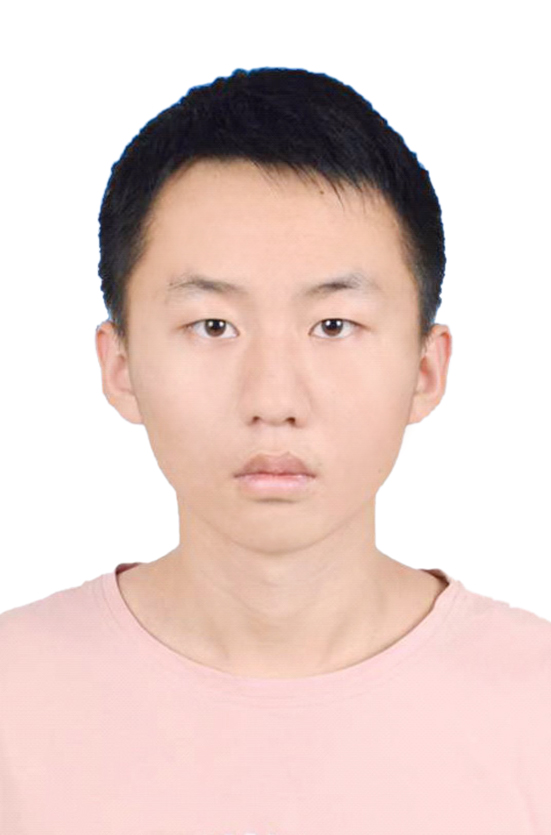
\includegraphics[width=1in,height=1.25in,clip,keepaspectratio]{assets/bio/yifei.jpg}}]{Yifei Gao} is pursuing the master degree at University College London. He previously obtained his B.Eng. degree from the College of Software Engineering at the University of Electronic Science and Technology of China in 2024. His current research interests encompass large language models, 3D reconstruction, and diffusion models.
\end{IEEEbiography}

\vspace{8pt}

\vspace{-33pt}

\begin{IEEEbiography}[{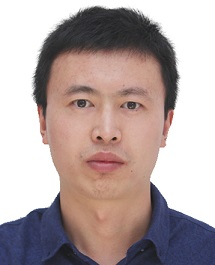
\includegraphics[width=1in,height=1.25in,clip,keepaspectratio]{assets/bio/leiwang.jpg}}]{Lei Wang} (Senior Member, IEEE) received the Ph.D. degree in Electrical Engineering from Xidian University, Xi'an, China, in 2010. From 2011 to 2012, he was with Huawei Technologies Company Ltd. From 2014 to 2015, he was with the Department of Embedded Systems Engineering, Incheon National University, as a Postdoctoral Fellow. He is currently an Associate Professor with the Shenzhen Institutes of Advanced Technology, Chinese Academy of Sciences, Shenzhen, China. He has authored or coauthored more than 70 papers in conferences and journals, including IEEE TRANSACTIONS ON CIRCUITS AND SYSTEMS FOR VIDEO TECHNOLOGY, IEEE TRANSACTIONS ON CYBERNETICS, IEEE TRANSACTIONS ON MULTIMEDIA, IEEE SIGNAL PROCESSING LETTERS, and NAACL. His research interests include image processing, transforms, machine learning, computer vision, 3-D reconstruction, and robotics.
\end{IEEEbiography}

\vspace{8pt}

\vspace{-33pt}

\begin{IEEEbiography}[{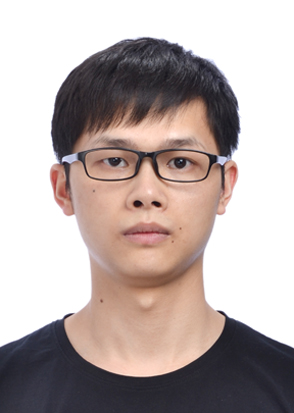
\includegraphics[width=1in,height=1.25in,clip,keepaspectratio]{assets/bio/rongcheng.jpg}}]{Rong-Cheng Tu}
received the B.S. degree in 2018 and the Ph.D. degree in 2023 from the Beijing Institute of Technology, Beijing, China. 
He is currently a Research Fellow with Nanyang Technological University (NTU), Singapore. 
His research interests include deep learning, information retrieval, and Large Language Model efficiency.
\end{IEEEbiography}

\vspace{8pt}

\vspace{-33pt}

\begin{IEEEbiography}[{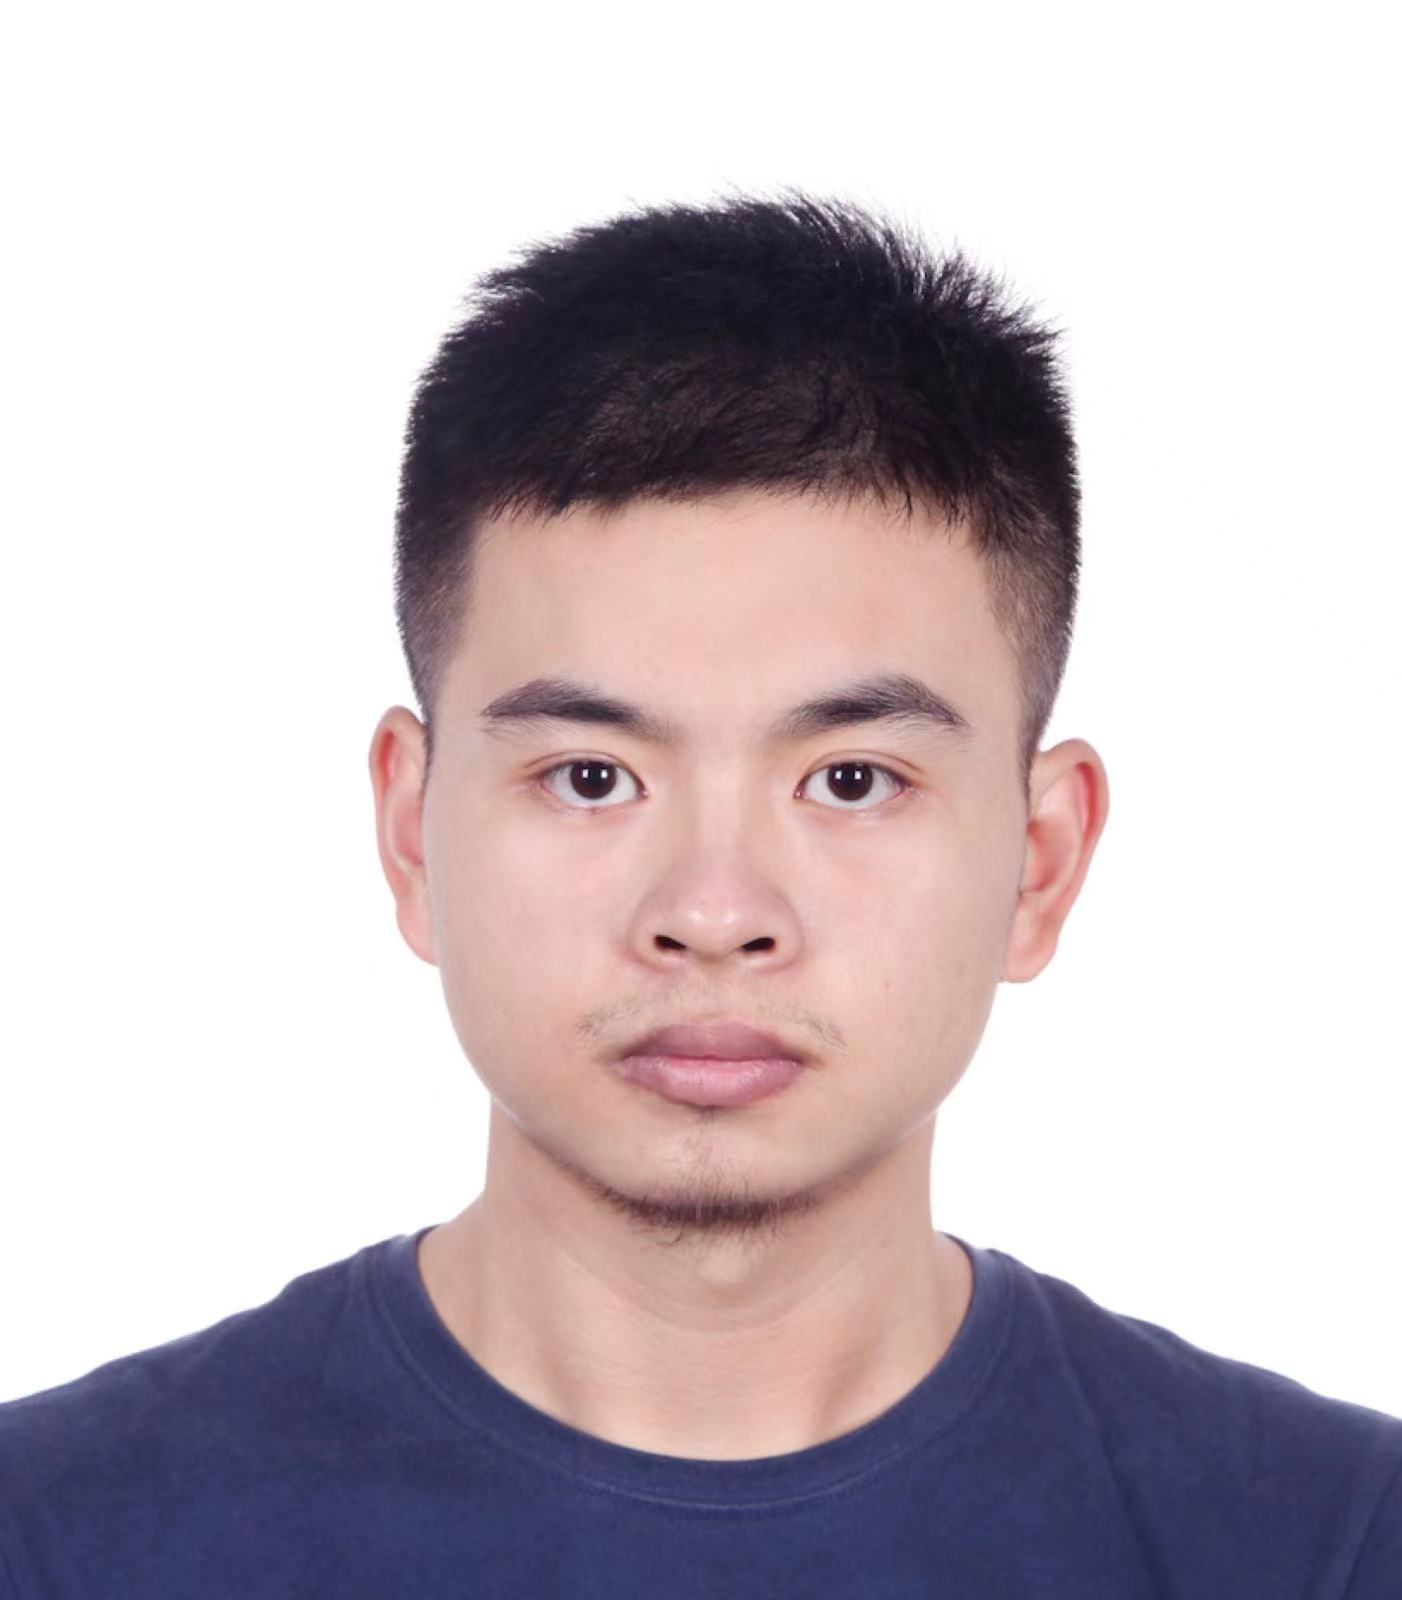
\includegraphics[width=1in,height=1.25in,clip,keepaspectratio]{assets/bio/qixin.jpg}}]{Qixin Zhang}
received his B.S. degree from the University of Science and Technology of China in 2018. He subsequently earned his Ph.D. degree in the School of Data Science at City University of Hong Kong in 2024. Currently, he is a Research Fellow at Nanyang Technological University, Singapore. His research interests include submodular optimization, subset selection and network prune. He has published over 15 papers in top data science venues such as ICML, NeurIPS, ICLR, AISTATS, AAAI and TKDE, etc.
\end{IEEEbiography}

\vspace{8pt}

\vspace{-33pt}

\begin{IEEEbiography}[{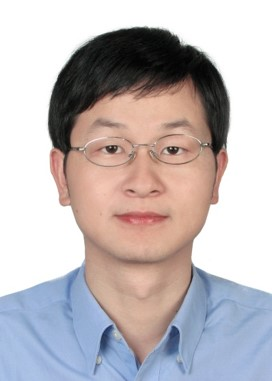
\includegraphics[width=1in,height=1.25in,clip,keepaspectratio]{assets/bio/juncheng.jpg}}]{Jun Cheng} (Senior Member, IEEE) received the B.Eng. and M.Eng. degrees from the University of Science and Technology of China, Hefei, China, in 1999 and 2002, respectively, and the Ph.D. degree from Chinese University of Hong Kong, Hong Kong, in 2006. He is currently a Professor with Shenzhen Institutes of Advanced Technology, Chinese Academy of Sciences, Shenzhen, China, where he is also the Director of the Laboratory for Human Machine Control. His current research interests include computer vision, robotics, machine intelligence, and control.
\end{IEEEbiography}

\vspace{8pt}

\vspace{-33pt}

\begin{IEEEbiography}[{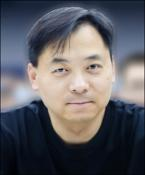
\includegraphics[width=1in,height=1.25in,clip,keepaspectratio]{assets/bio/dachengtao.jpeg}}]{Dacheng Tao} (F’15) is currently a Distinguished University Professor in the College of Computing \& Data Science at Nanyang Technological University. He mainly applies statistics and mathematics to artificial intelligence and data science, and his research is detailed in one monograph and over 200 publications in prestigious journals and proceedings at leading conferences, with best paper awards, best student paper awards, and test-of-time awards. His publications have been cited over 126K times and he has an hindex 160+ in Google Scholar. He received the 2015 and 2020 Australian Eureka Prize, the 2018 IEEE ICDM Research Contributions Award, and the 2021 IEEE Computer Society McCluskey Technical Achievement Award. He is a Fellow of the Australian Academy of Science, AAAS, ACM and IEEE.
\end{IEEEbiography}

\clearpage
\appendix

%\newpage
\subsection{Mean-shift Property of Token-sparse Attention}
\label{sec:mean-shift}

In this section, building upon prior research Deja Vu~\cite{liu2023deja}, we first describe the analytical foundation of our work: self-attention can be interpreted as a form of mean-shift clustering. Based on this perspective, we then explore the among-query properties of self-attention and leveraging the formal definition of TSA (as introduced in \textbf{Definition 3.1}) to construct and complete our theoretical proof.

\subsubsection{Self-Attention as Mean-Shift Clustering}


\paragraph{Implicit Clustering in Attention} The softmax weighting means that the query $\bq$ mainly focuses on a subset of keys with the largest dot-products $\bq \cdot \bk_j$. This behavior causes tokens to form clusters: tokens (keys) that are similar to a given query will receive high attention weights (“cluster members”), whereas unrelated tokens get negligible weight. In other words, each query \textbf{picks out clusters} of relevant key tokens and largely ignores the rest, which is exactly the token sparsity phenomenon~\cite{zhang2023h2o,tang2406quest} (only a few tokens significantly contribute to the attention result).

% Intuitively, $q$ will attend most to keys that are most similar to $q$ in the embedding space. 

% Notably, different attention heads learn different notions of similarity by projecting queries/keys into different subspaces; each head clusters tokens in its own projected space. After multiple layers, token embeddings themselves tend to form clusters as a result of these attention dynamics. Fig. 4 of the Deja Vu paper illustrates this: some heads concentrate their attention on specific tokens (“heavy hitters”~\cite{zhang2023h2o}) while others distribute it uniformly.

\paragraph{Mean-Shift Interpretation} 

Importantly, the Deja Vu study observed that \textbf{self-attention implements a one-step mean-shift clustering update}. Formally, fixing within one head, for the attention output $\by {=} \sum_{i} A_i (\bx_i \bW_V)$, if we ignore the $\bW_V$ projection for a moment, this computes the \emph{weighted centroid} of the token embeddings $\bx$ around the query $\bq$ (in the projected space). That is, define an \emph{attention mean} $m(\bq)$ as the weighted mean of the embeddings:
\begin{equation}
    m(q) \;=\; \frac{\sum_i \bK(\bx_i, \bq)\, \bx_i}{\sum_i \bK(\bx_i, \bq)}\,,
\end{equation}
so $\by {=} m(\bq) \bW_V$.  This is exactly the update step of the \textbf{mean-shift clustering algorithm}: $m(\bq)$ is pulling the query’s embedding toward a nearby cluster of points ${\bx_i}$ that are similar to $\bq$. In mean-shift, one would iteratively set $\bq \leftarrow m(\bq)$ to converge to the cluster center (mode of the density). In a Transformer, we usually apply just one such step per layer, but the analogy holds: \emph{each attention head nudges the query vector toward the centroid of a cluster of key vectors}.


\subsubsection{Among-Query Property}


\paragraph{Problem Setting} Consider two queries $\bq_t$ and $\bq_{t+1}$ from adjacent time steps in a sequence. Thanks to residual connections and the smooth nature of transformer dynamics, adjacent queries in a sequence tend to be close in embedding space~\cite{sun2024shadowkv,wuhshare}. We then assume as a general principle that \emph{$\bq_{t+1}$ is a small perturbation of $\bq_t$} (i.e. $\bq_{t+1} \approx \bq_t$ in $\ell_2$ norm or cosine similarity), as the among-query property only concerns the behavior of attention when queries are similar, we revise the \textbf{Among-query Property}~\ref{prop:among-query} that:

\begin{property}[Among-query Property]
\label{prop:among-query_new}
If two query vectors $\bq_t$ and $\bq_{t+1}$ are aligned enough in vector space, then the distributions of their attention weights are also very similar.
\end{property}

In other words, adjacent queries attend to largely the same cluster of key tokens. As $\bq_t$ shifts to $\bq_{t+1}$, the attention weight mass simply shifts smoothly among those keys–obeying a continuous mean-shift-like change–rather than jumping to a completely different set of keys.

\paragraph{Intuition via Mean-Shift} Think of the keys ${\bk_i}$ as data points in the embedding space. The query $\bq_t$ will put most weight on keys in some neighborhood (a “cluster”) around $\bq_t$. Now if $\bq_{t+1}$ moves slightly (say $\bq_{t+1} = \bq_t + \Delta$ for a small $\Delta$), it will still lie in roughly the same neighborhood of points. The attention kernel $\bK(x_i,\bq) = \exp(\bq\cdot \bk_i)$ is a smooth, continuous function of $q$. A slight change in $\bq$ causes only a slight change in all the similarity scores $\bq\cdot \bk_i$. Thus the weights $A_i$ shift slightly: keys that are highly ranked for $\bq_t$ will remain highly ranked for $\bq_{t+1}$, as long as $\bq_{t+1}$ hasn’t moved so far that it finds a totally different cluster.


\paragraph{Formal Derivation of the Among-Query Property}
\label{sec:among-query-def}
Let $\bK{=}\{\bk_1, \bk_2, \dots, \bk_t\}$ be the key vectors available. Consider two queries $\bq$ and $\bq'$ (think of $\bq = \bq_t$ and $\bq' = \bq_{t+1}$) such that $\bq'$ is a small perturbation of $\bq$. We will show that the attention distributions of $A(\bq)$ and $A(\bq')$ are \emph{close}, and in particular that the high-weight components of $A(\bq)$ correspond to high-weight components of $A(\bq')$. We also look at the weighted average outputs $\by(\bq)$ and $y(\bq')$. We first consider the perturbation changes in queries (e.g., $\bq$ to $\bq'$) to that of logits. For each key $\bk_i$, the score (logit) for $q$ as $a_i = \frac{1}{\sqrt{d}} \, \bq\cdot \bk_i$ and for $\bq'$ as $a'_i = \frac{1}{\sqrt{d}} \, \bq'\cdot \bk_i$. Because $\bq' = \bq + \Delta$ for a small $\Delta$, we have
$a'_j {-} a_j {=} \frac{1}{\sqrt{d}}(\bq' {-} \bq){\cdot} \bk_i {=} \frac{1}{\sqrt{d}} \Delta {\cdot} \bk_i$.

Let $\Delta_i := a'_i - a_i$. Since $| \Delta |$ is small and (typically) the keys ${\bk_i}$ have bounded norm, each $\Delta_i$ is a small real number. In other words, the entire vector of logits $a' = (a'_1,\dots,a'_t)$ is a small perturbation of $a = (a_1,\dots,a_t)$, and there exists some $\epsilon \ll 1$ such that $|\Delta_i| \le \epsilon$ for all $i$. ($\Delta_i$ might vary across $i$, but we can bound the maximum change by $\epsilon {=} \frac{|\Delta| \max_i|k_i|}{\sqrt{d}}$.) Then, combining the Softmax part in attention weights, by definition, $A_j(\bq) = \frac{e^{a_i}}{\sum_j e^{a_j}}$ and $A_j(\bq') = \frac{e^{a'*i}}{\sum_{j} e^{a'_j}}$. It will be convenient to express $A_i(\bq')$ in terms of $A(\bq)$ and the perturbations $\Delta_i$. We can write:
\begin{equation}
   A_i(\bq') = \frac{e^{a_i + \Delta_i}}{\sum_j e^{z_j + \Delta_j}} = \frac{e^{z_i}\,e^{\Delta_i}}{\sum_j e^{z_j}\,e^{\Delta_j}} = \frac{A_j(\bq)\,e^{\Delta_i}}{\sum_j A_j(\bq)\,e^{\Delta_j}}\,. 
\end{equation}
Here we use $e^{a_i}/\sum_j e^{a_j} = A_i(\bq)$ and factored $e^{\Delta_j}$ out of the denominator. Let $A^{n} = \sum_j A_j(q)\, e^{\Delta_i}$ denote the normalization factor that adjusts the weights due to the query change. Since each $\Delta_j$ is small, we can expand $A^{n}$ in a Taylor series:
\begin{equation}
\label{eq:d_taylor_exp}
\begin{aligned}
      A^{n} {=} \sum_j A_j(\bq)(1 {+} \Delta_j {+} O(\Delta_j^2)){=} 1 {+} \sum_j A_j(\bq)\Delta_j {+} O(\epsilon^2).  
\end{aligned}
\end{equation}
Here $\sum_j A_j(q)\Delta_j$ is the expectation of $\Delta$ under the original distribution $A(\bq)$. Let $\mu_\Delta {=} \sum_j A_j(q)\Delta_j$ for brevity. Combining Eq.~\eqref{eq:d_taylor_exp}, we can write $A^{n} {=} 1 {+} \mu_\Delta {+} O(\epsilon^2)$. Using this, we can approximate the new weights $A_i(\bq')$ based on the First-Order Taylor Approximation in small $\Delta$,
\begin{equation}
\begin{aligned}
\label{eq:d_first_order_taylor}
    A_i(\bq') \approx \frac{A_i(\bq)(1 {+} \Delta_i)}{1 + \mu_\Delta} \approx A_i(\bq)(1 {+} \Delta_i {-} \mu_\Delta),
\end{aligned}
\end{equation}
where second approximation used $\frac{1}{1+\mu_\Delta} \approx 1 - \mu_\Delta$ for small $\mu_\Delta$. Thus, for small query shifts, the new attention weight is approximately $A_i(\bq') {\approx} A_i(\bq) {+} A_i(\bq)(\Delta_i {-} \mu_\Delta)$. This formula reveals how the attention distribution shifts in response to $\Delta$:
\begin{itemize}[leftmargin=3mm]
    \item If $\Delta_i$ is larger than the average $\mu_\Delta$, then $A_i$ will increase ($\Delta_i - \mu_\Delta > 0$).
    \item If $\Delta_i$ is smaller than the average, $A_i$ will decrease slightly.
    \item The total change is zero-sum to first order as shown in Eq.~\eqref{eq:zero_sum}, as expected (the weights still sum to 1).
\end{itemize}
\begin{align}
\label{eq:zero_sum}
    &\sum_i [A_i(\bq') - A_i(\bq)] \approx \sum_i A_i(\bq)(\Delta_i - \mu_\Delta) \nonumber \\ 
    = &(\sum_i A_i(\bq)\Delta_i) - \mu_\Delta\sum_i A_i(\bq) =
    \mu_\Delta - \mu_\Delta(1) = 0
\end{align}

\paragraph{Transmission to Token-sparse Attention}

After proving the minimal attention score shifts in self-attention, we integrate them to the token-sparse attention defined in Sec.~\ref{sec:prob_def}. Suppose the original query $\bq$ had a set of critical keys (a cluster) $C = \{i : A_i(\bq)\}$ is among the top weights and above some importance threshold. We want to show that for $\bq'$, the high-weight keys $C' = \{i : A_i(\bq')\}$ largely overlap with $C$. From the approximation above, if $i {\in} C$ had a large original weight $A_i(\bq)$, then $A_i(\bq')$ will remain large unless something drastic happens to $\Delta_i$, as $\bq'{\cdot} \bk_i$ will remain relatively larger for those same $i{\in}C$ than for others.

For any $i$ in the original top cluster $C$, $a_i$ was high relative to most other $a_j$. The change $\Delta_i$ would have to be exceptionally negative (compared to others) to knock $i$ out of the top ranks. But $\Delta_i = \frac{1}{\sqrt{d}}\Delta {\cdot} \bk_i$ is small for all $i$, so it’s highly unlikely to completely invert the ordering of scores. In effect, the ranking of the top few $ A_i$ is stable under small perturbations of $\bq$. (One can make this rigorous by noting that softmax is a Lipschitz continuous function of its input logits; a sufficiently small change in $\bq$ cannot cause a large change in the output distribution. More concretely, if $| \Delta_i | < \delta$ for all $j$, then $\max_i |A_i(\bq') {-} A_i(\bq)|$ is $O(\delta)$ and the indices of the top weights cannot all change at once.) 

For any $i$ outside the cluster ($i {\notin} C$ with tiny $A_i(\bq)$), $\bq'$ would have to move much closer to $\bk_i$ (relative to the others) to elevate its weight significantly. A small $\Delta$ won’t make a previously irrelevant key suddenly important. Thus those outside keys remain with near-zero weight in $A(\bq')$. These observations imply $C'$ will contain $C$ or at least have large overlap. \textbf{Overall, $\bq$ and $\bq'$ induce very similar attention weight distributions.} Quantitatively, one could bound the KL-divergence or total variation between $A(\bq)$ and $A(\bq')$ in terms of $|\Delta|$. But the key point is that no single small $\Delta$ causes a big discrete jump in the distribution.

\paragraph{Smooth Shift of the Attention Centroid} 

Because the weight distribution shifts only slightly, the centroid (weighted average) of the attended keys also shifts smoothly. The output for query $q'$ is thus
\begin{equation}
\begin{aligned}
    \by(\,q') &= \sum_i [A_i(\bq) + A_i(\bq)(\Delta_i - \mu_\Delta)]\, \bk_i \\
    &\approx \sum_i A_i(\bq) \bk_i + \sum_i A_i(\bq)(\Delta_i - \mu_\Delta)\,\bk_i.
\end{aligned}
\end{equation}
The second term is a small adjustment. In fact, note that $\sum_i A_i(\bq)\Delta_i \bk_i {=} (\Delta {\cdot} \bk_i)$ weighted by $A_i$, this is roughly $\Delta$ projected onto the direction of the original output. Without going too deep into the algebra, the main result indicates that $\by(\bq') {-} \by(\bq)$ is of order $O(|\Delta|)$, a small change. Geometrically, if $\by(\bq)$ is (proportional to) the mean of cluster $C$, then $\by(\bq')$ will be the mean of almost the same cluster, just adjusted towards $\bq'$. \textbf{This is precisely what we expect from a mean-shift update: as the query moves, the cluster centroid moves along with it, continuously.}

% \paragraph{Conclusion of Proof} 

% We have shown that a small change in the query leads to a small change in the attention distribution $A(q)$. In particular, the identities of the keys with large attention weight remain mostly the same, and their weights adjust gradually. Thus, adjacent similar queries $q_t$ and $q_{t+1}$ will attend to an overlapping set of key tokens with smoothly varying weights. And this is the Among-Query Property for token-sparse attention: \emph{the cluster of critical tokens for $q_{t+1}$ is almost the same as that for $q_t$, shifting only slightly in a mean-shift fashion as the query embedding shifts.}


\subsubsection{Centroid Shift}
\label{sec:centroid-shift}

We formalize the Lipschitz continuity of the attention centroid with respect to the query. Follow the definition in Sec.~\ref{sec:among-query-def}, let $\{p_i\}_{i=1}^t\subset\mathbb{R}$ be scalar token positions (sequence coordinates), and define the sequence-axis centroid $c(\bq){=} \sum_{i=1}^t A_i(\bq)p_i$. Assume unit-norm queries ($\|\bq\|{=}\|\bq'\|{=}1$) so that $\|\bq'{-}\bq\|{=} \sqrt{2 {-} 2 \cos \angle(\bq,\bq')}$; non-normalized statements follow by the triangle inequality. We write $K_{\max}\!\stackrel{\mathrm{def}}{=}\!\max_i\|\bk_i\|$ and $\mathrm{diam}\,\mathcal{P}{=}\max_i p_i-\min_i p_i$.

\begin{lemma}[Softmax $\ell_\infty\!\to\!\ell_1$ Lipschitzness]
\label{lem:softmax-lip}
For any $a,a'\in\mathbb{R}^t$,
\[
\big \|\mathrm{softmax}(a')-\mathrm{softmax}(a)\big\|_1
\;\le\; 2\,\|a'-a\|_\infty.
\]
\end{lemma}

\begin{proof}
By the mean value theorem on the line segment between $a$ and $a'$, for some $\tilde a$ we have
$\mathrm{softmax}(a')- \mathrm{softmax}(a)= J(\tilde a)(a'-a)$, where
$J(\tilde a){=}\mathrm{diag}(A){-}AA^\top$ is the Jacobian at $\tilde a$ with
$A{=}\mathrm{softmax}(\tilde a)$. One checks that $\|J(\tilde a)\|_{\infty{\to}1}{\le} 2$ (equivalently, the total variation norm of the
softmax is $2$-Lipschitz with respect to $\ell_\infty$ perturbations of logits). Hence
$\|\mathrm{softmax}(a') {-} \mathrm{softmax}(a)\|_1 {\le} 2 \|a'-a\|_\infty$.
\end{proof}

\begin{lemma}[Logit change under query perturbation]
\label{lem:logit-perturb}
Let $\bq'=\bq+\Delta$. Then
\[
\|a(\bq')-a(\bq)\|_\infty
\;=\;
\max_{i}\frac{1}{\sqrt d}\,|\,\Delta^\top \bk_i\,|
\;\le\; \frac{K_{\max}}{\sqrt d}\,\|\Delta\|.
\]
\end{lemma}

\begin{proof}
Immediate from Cauchy–Schwarz: $|\Delta^\top \bk_i| \!\le\! \|\Delta\|\|\bk_i\|$.
\end{proof}

\begin{theorem}[Query-Lipschitz Centroid Drift]
\label{thm:centroid-lip}
For $\bq'{=}\bq{+}\Delta$,
\begin{equation}
\begin{aligned}
\big|c(\bq'){-}c(\bq)\big|
&\;\le\;
(\mathrm{diam}\,\mathcal{P})\cdot
\big\|A(\bq')-A(\bq)\big\|_1 \\
&\;\le\;
2\,(\mathrm{diam}\,\mathcal{P})\cdot \frac{K_{\max}}{\sqrt d}\,\|\Delta\|.
\end{aligned}
\end{equation}
In particular, $c(\bq') {=} c(\bq) {+} O(\|\Delta\|).$
\end{theorem}

\begin{proof}
By definition,
$|c(\bq')\!-\!c(\bq)|\le \|A(\bq')\!-\!A(\bq)\|_1 \cdot \max_i |p_i\!-\!\bar p|$ for any $\bar p$.
Choosing $\bar p\in[\min_i p_i,\max_i p_i]$ gives $\max_i|p_i-\bar p|\le \mathrm{diam}\,\mathcal{P}$, hence the first inequality. The second inequality follows by Lemmas~\ref{lem:softmax-lip} and \ref{lem:logit-perturb}.
\end{proof}

\iffalse
\paragraph{Key/Value-space centroid (optional).}
Define the key-space centroid $\bar k(q)=\sum_j A_j(q)k_j$. Then
\[
\|\bar k(q')-\bar k(q)\|
\;\le\; \sum_j \|k_j\|\,|A_j(q')-A_j(q)|
\;\le\; K_{\max}\,\|A(q')-A(q)\|_1
\;\le\; 2\,\frac{K_{\max}^2}{\sqrt d}\,\|\Delta\|.
\]
If values are used ($y_{\mathrm{out}}=\sum_j A_j(q)\,v_j$), replace $K_{\max}$ by
$V_{\max}=\max_j\|v_j\|$ to obtain
$\|y_{\mathrm{out}}(q')-y_{\mathrm{out}}(q)\|\le 2\,\frac{K_{\max}V_{\max}}{\sqrt d}\,\|\Delta\|$.
\fi

\subsubsection{CIS MI Bound Parameterization}
\label{sec:cis-mi-parameterization}

We connect CIS parameters $(\tau,m,r)$ to the pre–hoc retained-mass gap $\beta_{\mathrm{th}}$, which
feeds into the MI bound in Eq.~(\ref{eq:mi_bound}).

\paragraph{Notation}
Fix a head and a decoding step $t$. Let $\mathcal{S}_t^\ast(\bq)$ be the oracle top-$k$ set under query $\bq$,
sorted by attention weight. Let $\mathcal{S}_{t,m}(\bq)\subset\mathcal{S}_t^\ast(\bq)$ be its top-$m$ winners.
For an integer radius $r\ge 0$, define the $r$-neighborhood (on the sequence axis)
$\mathcal{N}_r(S)=\bigcup_{p\in S}\{p+\delta:\delta\in\{-r,\dots,r\}\}$ with clipping to $[1,t]$.
CIS reuses $\hat S_t(\bq) \;\stackrel{\mathrm{def}}{=}\; \mathcal{S}_t^\ast(\bq)\;\cup\;\mathcal{N}_r\!\big(\mathcal{S}_{t,m}(\bq)\big)$. For a later query $\bq'$ in the same block with cosine similarity $\mathsf{sim}(\bq,\bq')\ge \tau$, CIS uses $\hat S_t(\bq)$ as the shared index set for $\bq'$ (per Eq.~(\ref{eq:neighboring})). Define retained mass
$\tau_{\hat S_t}(\bq){=}\sum_{i{\in}\hat S_t(\bq)}A_i(\bq)$ and $\tau_{\mathrm{pre}}(\bq'){=}\sum_{i\in \hat S_t(\bq)}A_i(\bq')$, and the oracle mass $\tau^\ast(\bq') = \sum_{i\in \mathcal{S}_t^\ast(\bq')}A_i(\bq')$. Let $\Delta_{\mathrm{att}}(\tau)
{=} \big\|A(\bq'){-}A(\bq)\big\|_1$.

\begin{lemma}[Similarity ${\Rightarrow}$ attention variation]
\label{lem:sim-to-var}
If $\|\bq\|{=}\|\bq'\|{=}1$ and $\mathsf{sim}(\bq,\bq'){=}\cos\angle(\bq,\bq'){\ge} \tau$, then
\[
\Delta_{\mathrm{att}}(\tau)
\;\le\;
\frac{2K_{\max}}{\sqrt d}\,\|\bq'-\bq\|
\;=\;
\frac{2K_{\max}}{\sqrt d}\,\sqrt{2-2\tau}.
\]
\end{lemma}
\begin{proof}
Combine Lemmas~\ref{lem:softmax-lip}--\ref{lem:logit-perturb} and $\|\bq'{-}\bq\|{=}\sqrt{2{-}2\tau}$ for unit-norm queries.
\end{proof}

\begin{lemma}[Oracle continuity]
\label{lem:oracle-mass}
$\big|\tau^\ast(\bq'){-}\tau^\ast(\bq)\big|{\le} \Delta_{\mathrm{att}}(\tau)$.
\end{lemma}

\begin{proof}
For any fixed index set $S$, the map $q{\mapsto} \sum_{i\in S}A_i(\bq)$ is $1$-Lipschitz in total variation:
$\big|\sum_{i\in S}(A_i(\bq')-A_i(\bq))\big|\le \|A(\bq'){-}A(\bq)\|_1$.
Taking $S{=}\mathcal{S}^\ast_t(\bq')$ yields
$\tau^\ast(\bq') \le \sum_{i\in \mathcal{S}^\ast_t(\bq')} A_i(\bq) + \Delta_{\mathrm{att}}(\tau){\le} \tau^\ast(\bq){+}\Delta_{\mathrm{att}}(\tau)$.
By symmetry, also $\tau^\ast(\bq)\le \tau^\ast(\bq')+\Delta_{\mathrm{att}}(\tau)$.
\end{proof}

\begin{lemma}[Reuse lower bound]
\label{lem:reuse-lb}
$\tau_{\mathrm{pre}}(\bq') \ge \tau_{\hat S_t}(\bq)-\Delta_{\mathrm{att}}(\tau)$.
\end{lemma}
\begin{proof}
$\tau_{\mathrm{pre}}(\bq')- \tau_{\hat S_t}(\bq)=\sum_{j\in \hat S_t(\bq)}(A_i(\bq')-A_i(\bq))\ge -\|A(\bq'){-}A(\bq)\|_1$.
\end{proof}

\paragraph{Covering drift with radius $r$}
Observation~\ref{prop:among-query_new} and Theorem~\ref{thm:centroid-lip} imply that, along the sequence axis,
cluster centers move by at most
\[
\Delta_{\mathrm{centroid}}(\tau)
\;\le\; 2\,(\mathrm{diam}\,\mathcal{P})\cdot \frac{K_{\max}}{\sqrt d}\,\sqrt{2-2\tau}.
\]
Let $s(\tau)$ be any integer radius satisfying $s(\tau)\ge \Delta_{\mathrm{centroid}}(\tau)$.
If $r\ge s(\tau)$, $\mathcal{N}_r(\mathcal{S}_{t,m}(\bq))$ covers the mean shift of the dominant
modes between $\bq$ and $\bq'$; in particular, no additional loss is incurred from cluster translation outside $\hat S_t(\bq)$.

\begin{proposition}[Pre–hoc retained-mass gap under CIS]
\label{prop:cis-beta}
Assume $r\ge s(\tau)$ as above. Then
\begin{equation}
\begin{aligned}
\tau_{\mathrm{pre}}(\bq') &\;\ge\; \tau^\ast(\bq') - 2\,\Delta_{\mathrm{att}}(\tau),
 \\
\beta_{\mathrm{th}}(\bq') &\;\stackrel{\mathrm{def}}{=}\; \tau^\ast(\bq')-\tau_{\mathrm{pre}}(\bq') \;\le\; 2\,\Delta_{\mathrm{att}}(\tau).
\end{aligned}
\end{equation}
Consequently, with $L$ candidate indices and baseline truncation $\delta^\ast(\bq')$ from TSA,
\begin{equation}
\begin{aligned}
I_{\mathrm{full}}(\bq')-I_{\mathrm{pre}}(\bq')
&\;\le\; 2[h_b\!\Big(\delta^\ast(\bq')+2\,\Delta_{\mathrm{att}}(\tau)\Big) \\
&+ \Big(\delta^\ast(\bq')+2\,\Delta_{\mathrm{att}}(\tau)\Big)\log L].
\end{aligned}
\end{equation}

\end{proposition}

\begin{proof}
By Lemma~\ref{lem:reuse-lb}, $\tau_{\mathrm{pre}}(\bq') \ge \tau_{\hat S_t}(q)-\Delta_{\mathrm{att}}(\tau)$.
Since $\hat S_t(\bq)$ contains $\mathcal{S}_t^\ast(\bq)$ by definition, $\tau_{\hat S_t}(\bq)\ge \tau^\ast(\bq)$.
By Lemma~\ref{lem:oracle-mass}, $\tau^\ast(\bq)\ge \tau^\ast(q')-\Delta_{\mathrm{att}}(\tau)$.
Combine to get $\tau_{\mathrm{pre}}(\bq') \ge \tau^\ast(\bq')-2\,\Delta_{\mathrm{att}}(\tau)$.
The MI bound follows by substituting $\beta_{\mathrm{th}}(\bq')\le 2\,\Delta_{\mathrm{att}}(\tau)$ into Eq.~(\ref{eq:mi_bound}).
\end{proof}

\paragraph{When $r<s(\tau)$ (under-dilation)}
Define the residual drift loss as
\[
\varepsilon_{\mathrm{drift}}(\bq,\bq';m,r)
\;\stackrel{\mathrm{def}}{=}\;
\sum_{j\in \mathcal{N}_{s(\tau)}(\mathcal{S}_{t,m}(\bq))\setminus \mathcal{N}_{r}(\mathcal{S}_{t,m}(\bq))}
\hspace{-2mm}A_j(\bq)\,,
\]
i.e., the attention mass (under $\bq$) that can shift within $s(\tau)$ but lies outside the chosen radius $r$.
Then the same proof yields
\[
\beta_{\mathrm{th}}(\bq') \;\le\; 2\,\Delta_{\mathrm{att}}(\tau) \;+\; \varepsilon_{\mathrm{drift}}(\bq,\bq';m,r),
\]
and the MI bound holds with $\beta_{\mathrm{th}}$ replaced by the PrHS.
In practice we set $r\!=\!1$ and increase $m$ before $r$; this covers the dominant modes while keeping
$\varepsilon_{\mathrm{drift}}$ negligible and the workload
$\hat S_t\!\approx C_{\mathrm{sink}}+C_{\mathrm{local}}+k+m(2r)$ small.




\subsection{Exponential Recency Beyond Sink}
\label{sec:exp-decay}
We adopt RoPE positional embeddings~\cite{su2024roformer} and analyze their interaction with self-attention~\cite{vaswani2017attention}. Excluding sink tokens, the multi-frequency rotations in RoPE cause phase dispersion with distance: representations of far-apart tokens become increasingly orthogonal in the rotated space, sharply reducing similarity (a \emph{long-term decay} effect). Softmax attention amplifies this decay and translate it into exponentially smaller attention weights. Empirically, attention scores decrease roughly linearly or sublinearly with distance to the current token, while attention probabilities decay exponentially or faster, consistent with prior measurements~\cite{zhang2023h2o,xiao2023streamingllm}. Thus, we assume there exist layer-dependent constants $\lambda_\ell>0$ and a factor
$\kappa_\ell\in(0,1]$ such that for all $i>C_{\text{sink}}$,
\begin{equation}
\label{eq:exp-decay}
A^{(\ell)}_i(\bq^{(\ell)}_t)
\ \le\
\kappa_\ell\,(1-\rho_\ell)\,\rho_\ell^{\,t-i},
\quad \rho_\ell \stackrel{\mathrm{def}}{=} e^{-\lambda_\ell}\in(0,1).
\end{equation}
Equivalently, the non-sink portion of $A^{(\ell)}$ is dominated pointwise by a geometric tail with ratio $\rho_\ell$ and mass $\kappa_\ell$. 

In addition, the similarity of cross-layer hidden states (including keys and values) can exceed 95\% beyond certain layer depth (generally with $\ell{>}N/2$)~\cite{liu2405minicache}. We then assume: for the per-layer key update $\Delta\bk^{(\ell)}_i
\stackrel{\mathrm{def}}{=}\bk^{(\ell)}_i-\bk^{(\ell-1)}_i$, there exist
$B>0$ and $\mu>0$ such that for the prefix to be frozen at layer $\ell$,
\begin{equation}
\label{eq:cross-layer-update}
\max_{1\le i\le E_\ell(t)} \big\|\Delta\bk^{(\ell)}_i\big\|
\ \le\
B\,e^{-\mu\,(\ell-\ell_s)}
\end{equation}


\begin{lemma}[Logit change under key perturbations]
\label{lem:logitDelta}
Let $a_i=\tfrac{1}{\sqrt d}(\bq^\top \bk_i)$ and
$a'_i=\tfrac{1}{\sqrt d}(\bq^\top \bk'_i)$. Then
\[
\|a'-a\|_\infty
\ \le\ \frac{\|\bq\|}{\sqrt d}\,\max_i\|\bk'_i-\bk_i\|.
\]
\emph{Proof.} Immediate from Cauchy--Schwarz. \qedhere
\end{lemma}

\subsection{PSAW Bounds on Dropped Mass}
\label{sec:psaw-bound}

Following the PSAW selector defined in Sec.~\ref{sec:psaw}, and dropped set $\mathcal{D}_\ell=\{C_{\text{sink}}+1,\dots,P_\ell(t)-1\}$.
The dropped mass at layer $\ell$ is $\delta^{\mathrm{PSAW}}_\ell
\stackrel{\mathrm{def}}{=}\sum_{i\in\mathcal{D}_\ell} A^{(\ell)}_i(\bq^{(\ell)}_t)$. Let the window-start distance $D_\ell\stackrel{\mathrm{def}}{=} t-P_\ell(t)+1$ and satisfies $D_\ell\ge \lfloor u_\ell t\rfloor$.

\begin{theorem}[PSAW worst-case bound]
\label{thm:PSAW}
Under~\eqref{eq:exp-decay}, for every $\ell\ge\ell_s$,
\[
\delta^{\mathrm{PSAW}}_\ell
\ \le\
(1-\tau^{(\ell)}_{\mathrm{sink}})\,e^{-\lambda_\ell\,D_\ell}
\ \le\
e^{-\lambda_\ell\,D_\ell}.
\]
\emph{Proof.}
Reindex non-sink positions by distance $d=t-i\in\{0,1,2,\dots\}$. Then $\mathcal{D}_\ell$ corresponds to $d\ge D_\ell$ and
\begin{equation}
\begin{aligned}
\delta^{\mathrm{PSAW}}_\ell
&=\sum_{i\in\mathcal{D}_\ell}A^{(\ell)}_i
\ \le\
\kappa_\ell\sum_{d\ge D_\ell}(1-\rho_\ell)\rho_\ell^{\,d} \\
&=\kappa_\ell\,\rho_\ell^{\,D_\ell}
=\kappa_\ell\,e^{-\lambda_\ell D_\ell}.
\end{aligned}
\end{equation}
Since $\kappa_\ell\le 1-\tau^{(\ell)}_{\mathrm{sink}}\le 1$ the claim follows.
\qedhere
\end{theorem}

For the top layer $\ell=N$, $u_N=\phi^\alpha$ and $D_N\ge \lfloor \phi^\alpha t\rfloor$, we then have
\[
\delta^{\mathrm{PSAW}}_N
\ \le\
(1-\tau^{(N)}_{\mathrm{sink}})\,e^{-\lambda_N\,\lfloor \phi^\alpha t\rfloor}
\ \le\
e^{-\lambda_N\,\phi^\alpha t}.
\]
Given a target budget $\beta^{\mathrm{PSAW}}\in(0,1)$, any $(\phi,\alpha)$ satisfying
\[
\phi^\alpha
\ \ge\
\frac{1}{\lambda_N t}\,\log\!\frac{1}{\beta^{\mathrm{PSAW}}/(1-\tau^{(N)}_{\mathrm{sink}})}
\]
ensures $\delta^{\mathrm{PSAW}}_N\le \beta^{\mathrm{PSAW}}$. Otherwise, if $\lambda_\ell \ge \underline{\lambda}>0$ almost surely and
$\mathbb{E}[1-\tau^{(\ell)}_{\mathrm{sink}}]\le 1$, then
\[
\mathbb{E}\big[\delta^{\mathrm{PSAW}}_\ell\big]
\ \le\
\mathbb{E}\big[(1-\tau^{(\ell)}_{\mathrm{sink}})\big]\,e^{-\underline{\lambda}\,D_\ell}
\ \le\
e^{-\underline{\lambda}\,D_\ell}.
\]

\subsection{ETF Bounds on Additional Mass Gap}
\label{sec:etf-bound}
For ETF define in Sec.~\ref{sec:etf}, freezing means: for $i\le E_\ell(t)$, set
$\bk^{(\ell)}_i\leftarrow \bk^{(\ell-1)}_i$ and $\bv^{(\ell)}_i\leftarrow \bv^{(\ell-1)}_i$; for $i> E_\ell(t)$, compute as usual. Let $A^{(\ell)}$ denote the full (unfrozen) attention distribution and
$\widetilde A^{(\ell)}$ the distribution under ETF at layer $\ell$. Define the ETF-induced mass gap (a total-variation budget)
\[
\beta^{\mathrm{ETF}}_\ell(\bq^{(\ell)}_t)
\ \stackrel{\mathrm{def}}{=}\ \frac12\big\|\,\widetilde A^{(\ell)}(\bq^{(\ell)}_t)-A^{(\ell)}(\bq^{(\ell)}_t)\big\|_1.
\]

\begin{theorem}[ETF: per-layer worst-case bound]
\label{thm:ETF}
Following~\eqref{eq:cross-layer-update} and $\|\bq^{(\ell)}_t\|\le Q_{\max}$. Then
\[
\beta^{\mathrm{ETF}}_\ell(\bq^{(\ell)}_t)
\ \le\
\frac{Q_{\max}}{\sqrt d}\,B\,e^{-\mu\,(\ell-\ell_s)}.
\]
\emph{Proof.}
Let $a_i=\frac{1}{\sqrt d}(\bq^{(\ell)}_t)^\top \bk^{(\ell)}_i$
and $\tilde a_i=\frac{1}{\sqrt d}(\bq^{(\ell)}_t)^\top \tilde \bk^{(\ell)}_i$, where
$\tilde \bk^{(\ell)}_i=\bk^{(\ell-1)}_i$ if $i\le E_\ell(t)$ and
$\tilde \bk^{(\ell)}_i=\bk^{(\ell)}_i$ otherwise. Then $\Delta a_i=\tilde a_i-a_i=-\frac{1}{\sqrt d}(\bq^{(\ell)}_t)^\top \Delta\bk^{(\ell)}_i$
for $i\le E_\ell(t)$ and $0$ otherwise.
By Lemma~\ref{lem:logitDelta} and~\eqref{eq:cross-layer-update},
\begin{equation}
\begin{aligned}
\|\tilde a-a\|_\infty
{\le}
\frac{\|\bq^{(\ell)}_t\|}{\sqrt d}
\max_{1\le i \le E_\ell(t)} \|\Delta\bk^{(\ell)}_i\|
{\le}
\frac{Q_{\max}}{\sqrt d}\,B\,e^{-\mu(\ell-\ell_s)}
\end{aligned}
\end{equation}
By Lemma~\ref{lem:softmaxLip},
$\|\widetilde A^{(\ell)}-A^{(\ell)}\|_1 \le 2 \|\tilde a-a\|_\infty$,
hence
$\|\widetilde A^{(\ell)}-A^{(\ell)}\|_1
\le 2 \frac{Q_{\max}}{\sqrt d}\,B\,e^{-\mu(\ell-\ell_s)}$.
Divide by $2$ to obtain the claim.
\qedhere
\end{theorem}

On the other hand, if $\mathbb{E}\|\bq^{(\ell)}_t\|\le \bar Q$, then
\[
\mathbb{E}\big[\beta^{\mathrm{ETF}}_\ell\big]
\ \le\
\frac{\bar Q}{\sqrt d}\,B\,e^{-\mu(\ell-\ell_s)}.
\]

\subsection{Joint pre-hoc retained-mass certificate and tuning}

At layer $\ell$, the overall pre-hoc mass budget from PSAW and ETF satisfies
\begin{equation}
\begin{aligned}
\delta^{\mathrm{(PSAW+ETF)}}_\ell
& \le
\underbrace{\delta^{\mathrm{PSAW}}_\ell}_{\text{masking}}
+
\underbrace{\beta^{\mathrm{ETF}}_\ell}_{\text{freezing perturbation}} \\
& \le
(1-\tau^{(\ell)}_{\mathrm{sink}})e^{-\lambda_\ell D_\ell} +
\frac{Q}{\sqrt d}\,B\,e^{-\mu(\ell-\ell_s)},  
\end{aligned}
\end{equation}
where $Q\in\{Q_{\max},\bar Q\}$ depending on worst/average case. And at the top layer $\ell=N$,
$\delta^{\mathrm{PSAW+ETF}}_N
\ \le\
(1-\tau^{(N)}_{\mathrm{sink}})\,e^{-\lambda_N \lfloor \phi^\alpha t\rfloor}
\ +\
\frac{Q}{\sqrt d}\,B\,e^{-\mu(N-\ell_s)}.$

In practice, given targets $\beta^{\mathrm{PSAW}},\beta^{\mathrm{ETF}}\in(0,1)$, it suffices to choose
$(\phi,\alpha)$ and $(\psi,\gamma)$ under average case such that
\[
(1-\tau^{(N)}_{\mathrm{sink}})\,e^{-\underline{\lambda}_N \lfloor \phi^\alpha t\rfloor}
\le \beta^{\mathrm{PSAW}},
\,\,
\frac{\bar Q}{\sqrt d}\,B\,e^{-\mu(N-\ell_s)}
\le \beta^{\mathrm{ETF}}.
\]
Equivalently,
\[
\phi^\alpha
\ge
\frac{1}{\underline{\lambda}_N t}\,\log\!\frac{1-\tau^{(N)}_{\mathrm{sink}}}{\beta^{\mathrm{PSAW}}},
\quad
N-\ell_s
\ge
\frac{1}{\mu}\,\log\!\frac{\bar Q B}{\beta^{\mathrm{ETF}}\sqrt d}.
\]

%\end{thebibliography}


\vfill

\end{document}


